\documentclass[a4paper]{article}
\usepackage{import}
\usepackage[utf8]{inputenc}
\usepackage[T1]{fontenc}
\usepackage{textcomp}
\usepackage[italian]{babel}
\usepackage{amsmath, amssymb}
\usepackage{booktabs,xltabular}
\usepackage{amsfonts}
\usepackage{subcaption}
\usepackage{amsthm}
\usepackage{cancel}
\usepackage{mdframed}
\usepackage{makecell}
\usepackage{float}
\usepackage{xcolor}
\usepackage{listings}
\usepackage{gensymb}
\usepackage{graphicx}
\usepackage{bodeplot}
\usepackage{physics}
\usepackage{tikz}
\usetikzlibrary{shapes, arrows, automata, petri, decorations.markings, decorations.pathreplacing, positioning, calc, quotes}
\usepackage{circuitikz}
\usepackage[label=corner]{karnaugh-map}
\graphicspath{{./figures/}}

% Set default font to sans-serif
\renewcommand{\familydefault}{\sfdefault} 
\usepackage{eulervm}

\usepackage{forest}

\usepackage{mathtools}
\DeclarePairedDelimiter\ceil{\lceil}{\rceil}
\DeclarePairedDelimiter\floor{\lfloor}{\rfloor}

% \usepackage{ntheorem}

\usepackage{import}
\usepackage{pdfpages}
\usepackage{transparent}
\usepackage{xcolor}

\usepackage{hyperref}
\hypersetup{
    colorlinks=false,
}

% Code blocks
\definecolor{codegreen}{rgb}{0,0.6,0}
\definecolor{codegray}{rgb}{0.5,0.5,0.5}
\definecolor{codepurple}{rgb}{0.58,0,0.82}
\definecolor{backcolour}{rgb}{0.95,0.95,0.95}

\lstdefinestyle{mystyle}{
	backgroundcolor=\color{backcolour},
	commentstyle=\color{codegreen},
	keywordstyle=\color{magenta},
	numberstyle=\tiny\color{codegray},
	stringstyle=\color{codepurple},
	basicstyle=\ttfamily\footnotesize,
	breakatwhitespace=false,
	breaklines=true,
	captionpos=b,
	keepspaces=true,
	numbers=left,
	numbersep=5pt,
	showspaces=false,
	showstringspaces=false,
	showtabs=false,
	tabsize=2
}

\lstset{style=mystyle}

\usepackage{color}
\usepackage{import}
\usepackage{pdfpages}
\usepackage{transparent}
\usepackage{xcolor}

% Example frame
\theoremstyle{definition}
\newmdtheoremenv[%
	linecolor=gray,leftmargin=0,%
	rightmargin=0,
	innertopmargin=8pt,%
	innerbottommargin=8pt,
	ntheorem]{example}{Esempio}[section]

% Important definition frame
\theoremstyle{definition}
\newmdtheoremenv[%
	linecolor=gray,leftmargin=0,%
	rightmargin=0,
	backgroundcolor=gray!40,%
	innertopmargin=8pt,%
	innerbottommargin=8pt,
	ntheorem]{definition}{Definizione}[section]

% Exercise frame
\theoremstyle{definition}
\newmdtheoremenv[%
	linecolor=gray,leftmargin=0,%
	rightmargin=0,
	innertopmargin=8pt,%
	innerbottommargin=8pt,
	ntheorem]{exercise}{Esercizio}[section]

% Theorem frame
\theoremstyle{definition}
\newmdtheoremenv[%
  linecolor=gray,leftmargin=0,%
  rightmargin=0,
  innertopmargin=8pt,%
  innerbottommargin=8pt,
  ntheorem]{theorem}{Teorema}[section]

\theoremstyle{definition}
\newmdtheoremenv[%
  linecolor=white,leftmargin=0,%
  rightmargin=0,
  innertopmargin=8pt,%
  innerbottommargin=8pt,
  ntheorem]{define}{Definizione utile}[section]

% figure support
\usepackage{import}
\usepackage{xifthen}
\pdfminorversion=7
\usepackage{pdfpages}
\usepackage{transparent}
\newcommand{\incfig}[1]{%
	\def\svgwidth{\columnwidth}
	\import{./figures/}{#1.pdf_tex}
}

% FSM tikz
\tikzset{
    place/.style={
        circle,
        thick,
        draw=black,
        minimum size=6mm,
    },
        state/.style={
        circle,
        thick,
        draw=black,
        fill=white,
        minimum size=6mm,
    },
}

\pdfsuppresswarningpagegroup=1

\usepackage{pgfplots}
\pgfplotsset{compat=1.18,width=10cm}

% Save plots as pdf and reuse them without compiling every time
\usetikzlibrary{external}
\tikzexternalize[prefix=figures/tikz/, optimize=false]


\begin{document}

\begin{titlepage}
	\begin{center}
		\vspace*{1cm}

		\Huge
		\textbf{Probabilità e Statistica\\Esercizi}

		\vspace{0.5cm}
		\LARGE
		UniVR - Dipartimento di Informatica

		\vspace{1.5cm}

		\textbf{Fabio Irimie}

		\vfill


		\vspace{0.8cm}


		2° Semestre 2023/2024

	\end{center}
\end{titlepage}


\tableofcontents
\pagebreak

\section{Introduzione}
Il problema principale che bisogna affrontare è la comunicazione tra 2 calcolatori,
cioè lo scambio di informazioni. Per far comunicare 2 calcolatori c'è bisogno di
alcuni requisiti:
\begin{enumerate}
  \item \textbf{Protocollo}: È un insieme di regole che sovraintende alla comunicazione,
    in cui si definiscono:
    \begin{itemize}
      \item Il formato dei messaggi
      \item Le azioni da intraprendere nel gestire i messaggi stessi
    \end{itemize}
    Questo perchè per comunicare tutti devono "parlare la stessa lingua".

  \item \textbf{Architettura di rete}: Come, fisicamente, trasportare i messaggi
\end{enumerate}

\begin{figure}[H]
  \begin{example}
    Prendiamo ad esempio la scrittura e la spedizione delle lettere. Ci sono 2
    utenti che vogliono scambiare delle lettere.
    
    Per gestire il trasporto della
    lettera essa viene messa all'interno di una \textbf{busta}, che contiene informazioni
    su dove deve essere spedita. Una volta inbustata, va imbucata in una cassetta 
    delle lettere da cui poi verrà prelevata e mandata alla cassetta delle lettere 
    del secondo utente dalla \textbf{rete} di distribuzione degli uffici postali.

    L'utente poi preleverà la lettera dalla cassetta delle lettere e dopo aver
    controllato le informazioni sulla busta, la aprirà e leggerà il contenuto.
    \begin{figure}[H]
      \centering
      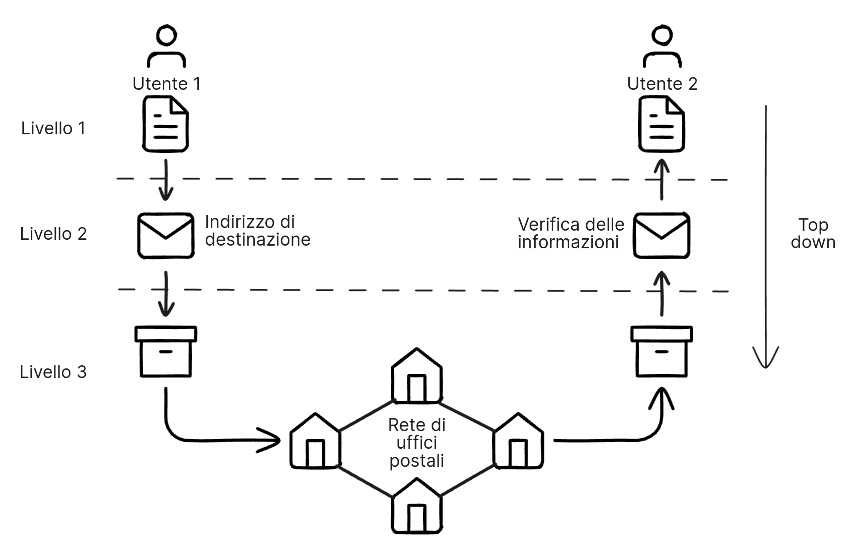
\includegraphics[width=0.95\textwidth]{rete-postale}
      \caption{Esempio di comunicazione tra 2 utenti}
    \end{figure}

    Il \textbf{Protocollo} è il linguaggio utilizzato per comunicare tra i 2
    utenti, mentre l'\textbf{Architettura di rete} è tutta quella infrastruttura
    che trasporta il messaggio tra i 2 utenti.
  \end{example}
\end{figure}

\noindent
La rappresentazione dei sistemi di comunicazione di solito viene fatta nella modalità
\textbf{top-down}, cioè si parte dal livello applicativo, quello più alto, fino a scendere
nei livelli più bassi in cui si trova la vera e propria architettura della rete.

\section{Architetture di rete}
Di solito si fa riferimento all'architettura più utilizzata, cioè la rete
\textbf{Internet}. Si possono distinguere i seguenti elementi base:
\begin{itemize}
  \item \textbf{Calcolatori (End host)}
  \item \textbf{Router (Intermediate host)}
  \item \textbf{Collegamenti}
\end{itemize}

\subsection{Reti locali}
Le reti locali, o \textbf{LAN} (Local Area Network), sono caratterizzate da un
\textbf{router di bordo} a cui sono collegati gli end host tramite \textbf{cavi fisici}
o collegamenti wireless.
\begin{figure}[H]
  \centering
  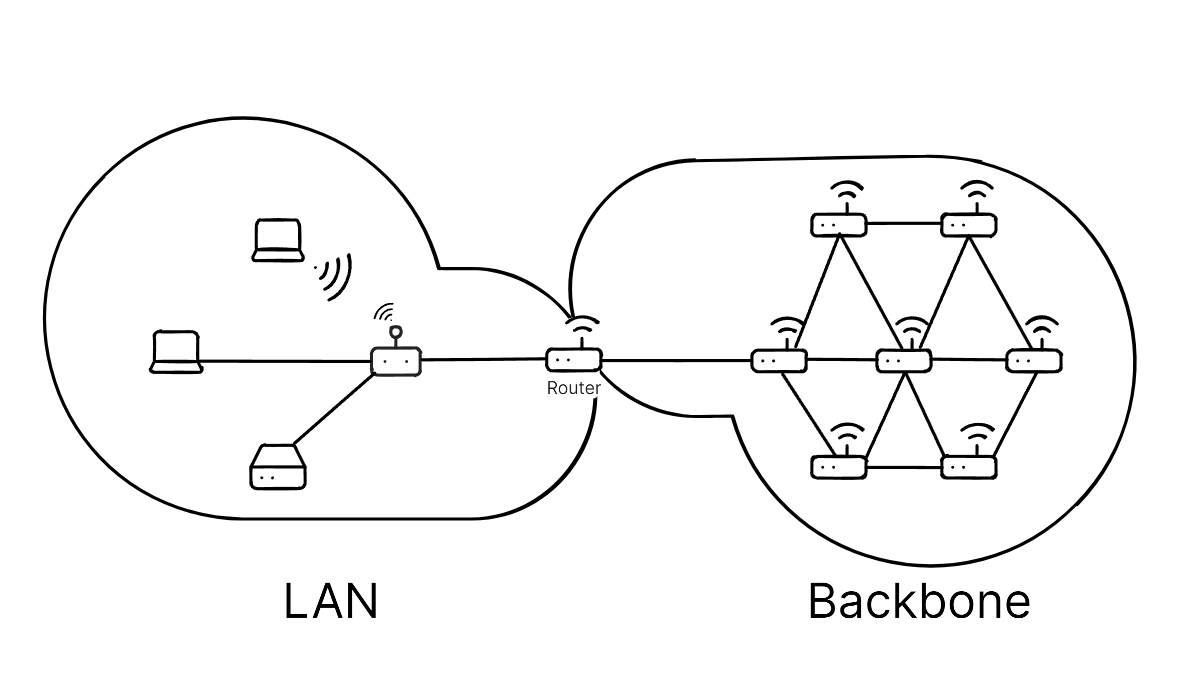
\includegraphics[width=0.95\textwidth]{lan-backbone}
  \caption{Rete locale}
\end{figure}

\vspace{1em}
\noindent
Per collegare diverse LAN tra loro esiste la \textbf{backbone}, cioè è una rete
di router collegati tra di loro con una topologia
gestita dal gestore della rete. Questi router sono geograficamente distribuiti
su tutto il territorio.
\begin{figure}[H]
  \centering
  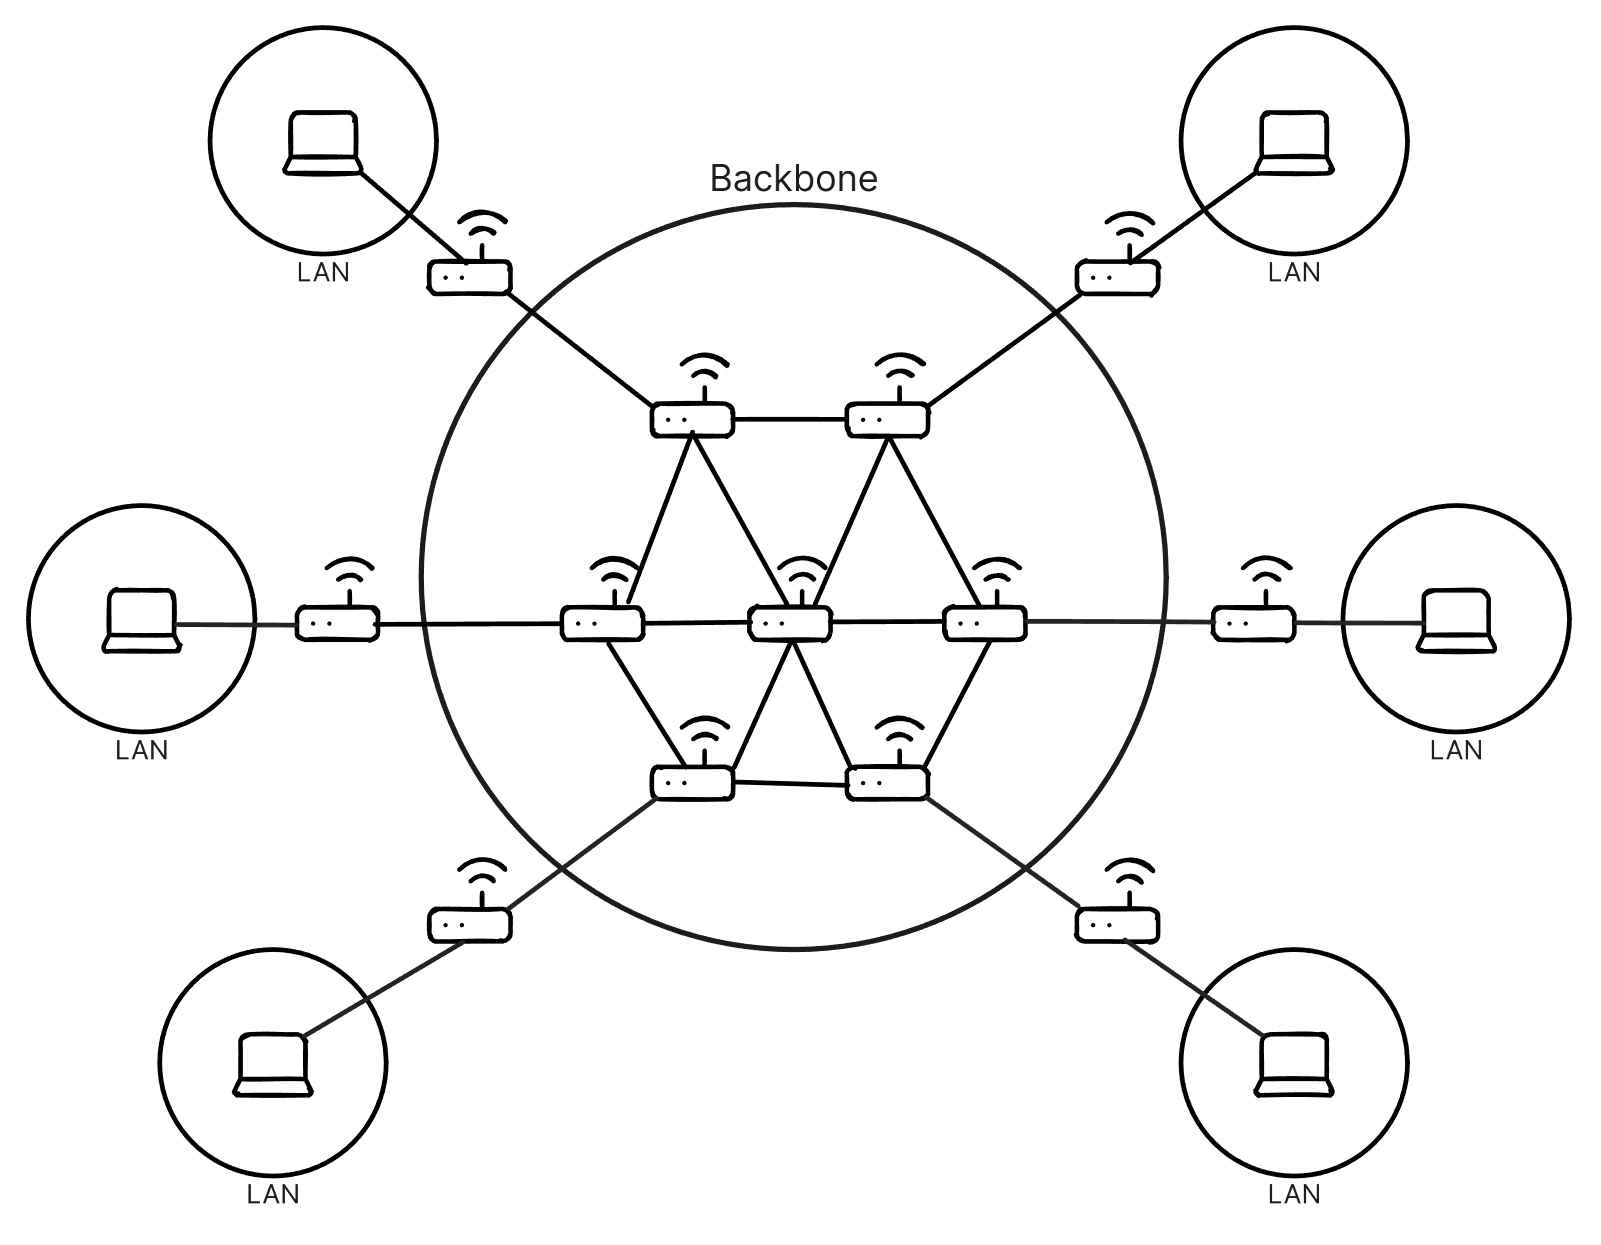
\includegraphics[width=0.95\textwidth]{internet}
  \caption{Intercollegamento di LAN}
\end{figure}

\noindent
Nella maggior parte delle volte le connessioni tra i router all'interno della
backbone sono cablate, di solito tramite fibre ottiche, soltanto in rari casi
si usano connessioni wireless.

\subsubsection{Organizzazione del Backbone}
Il backbone è composto da diverse reti che appartengono a diverse organizzazioni
permettendo di creare diverse interconnessioni tra le reti. Queste organizzazioni
si chiamano \textbf{Internet Service Provider} (ISP). Gli ISP hanno diversi livelli:
\begin{enumerate}
  \item \textbf{Livello 1}: Hanno una connessione internazionale
    e quindi sono in grado di comunicare con tutti gli altri ISP.
  \item \textbf{Livello 2}: Lavorano a livello nazionale.
  \item \textbf{Livello 3}: Lavorano a livello locale.
\end{enumerate}

\noindent
Gli ISP di livello 1 sono collegati tra di loro per permettere la comunicazione
tra ISP di livello 1 diversi. Anche gli ISP di livello più basso permettono
la comunicazione tra di loro o tra gli ISP di livello superiore, tutto questo
grazie ad accordi commerciali tra le varie organizzazioni.
\begin{figure}[H]
  \centering
  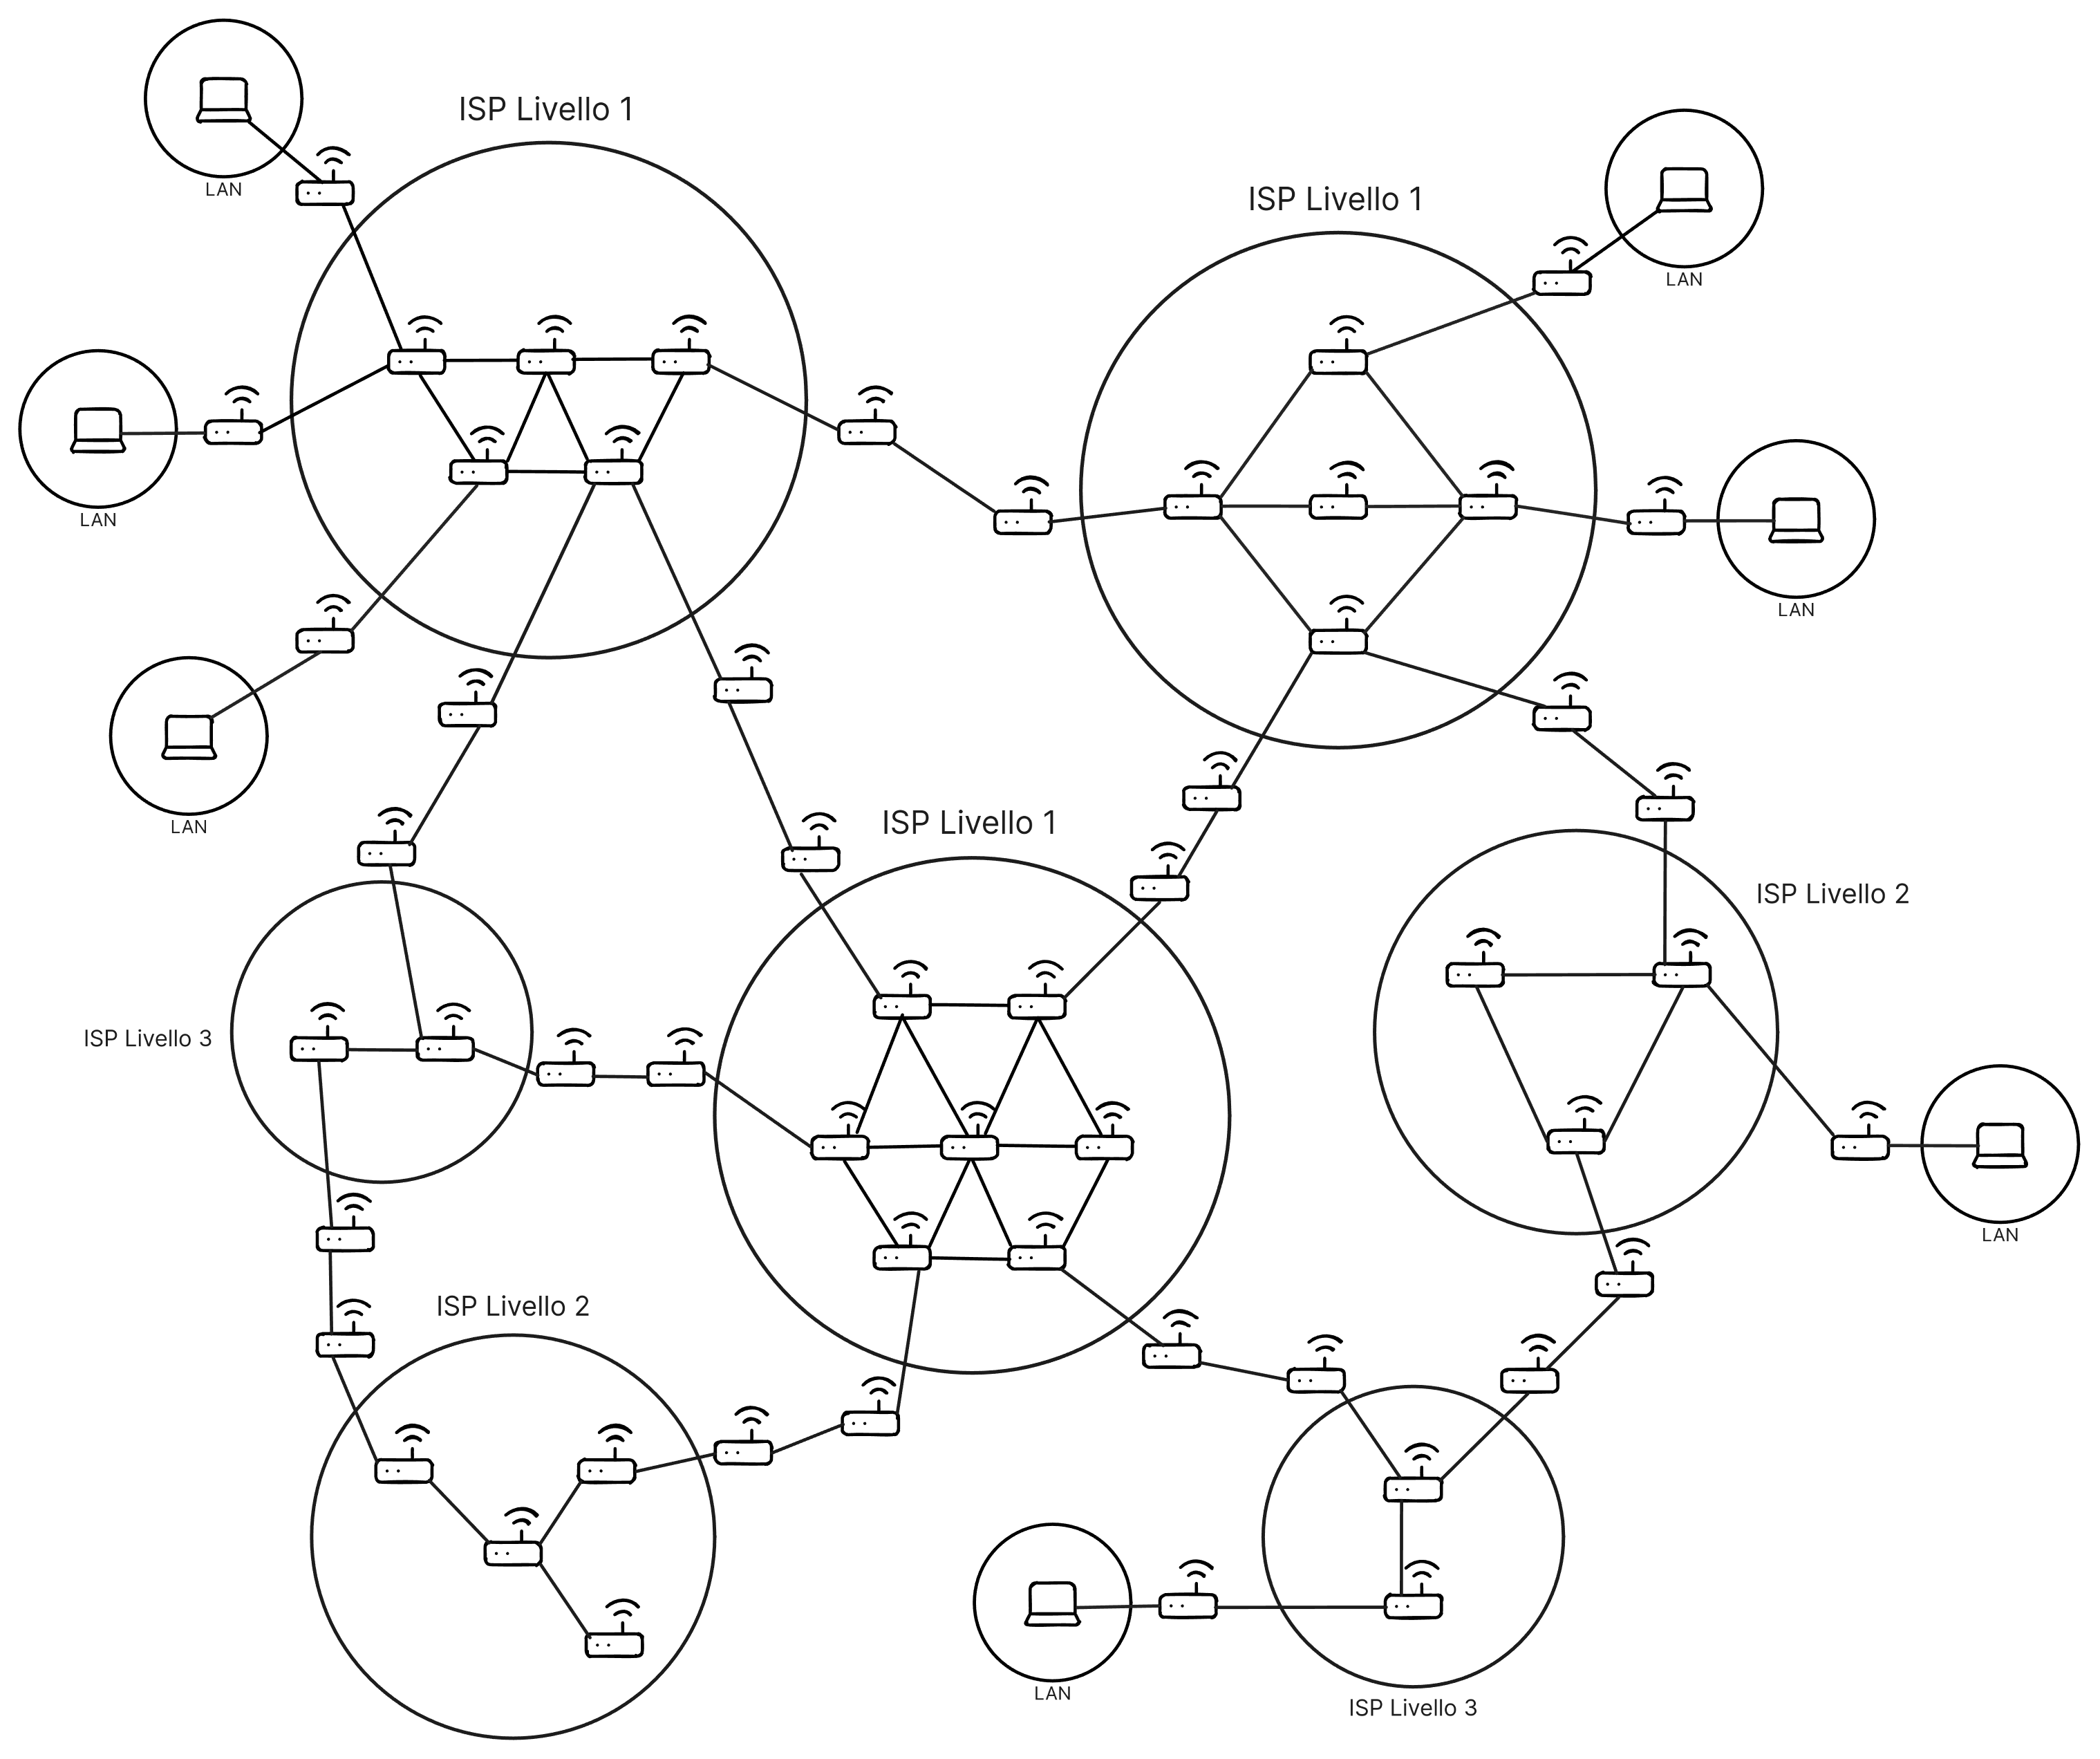
\includegraphics[width=0.95\textwidth]{livelli-di-isp}
  \caption{Livelli di ISP}
\end{figure}

\noindent
\textbf{Internet} è la \textbf{Rete delle reti}, cioè è la rete che collega
tutti gli ISP tra di loro ed è un organizzazione gerarchica, cioè è sufficiente
creare collegamenti con un sottoinsieme di ISP operanti sul territorio per permettere
il collegamento a tutta la rete.

\noindent
Di conseguenza, per raggiungere un utente, in genere, si segue un percorso gerarchico.
Un esempio è la rete stradale, dove per raggiungere una città si seguono le strade
principali e poi si scende in quelle secondarie.

\noindent
La scelta del percorso segue criteri basati su distanza e tempo.

\section{Modalità di comunicazione}
La gestione del trasporto dei messaggi è gestita dalla rete, però con che modalità
trasferisco l'informazione tra 2 utenti?

\subsection{Reti a commutazione di circuito}
È la modalità di commutazione che è stata utilizzata per la prima volta.

\noindent
In questa modalità le risorse (capacità del canale di trasmissione) vengono riservate \textbf{end-to-end}
per la comunicazione, cioè viene letteralmente riservato un circuito che viene
utilizzato dai 2 utenti.
\begin{figure}[H]
  \centering
  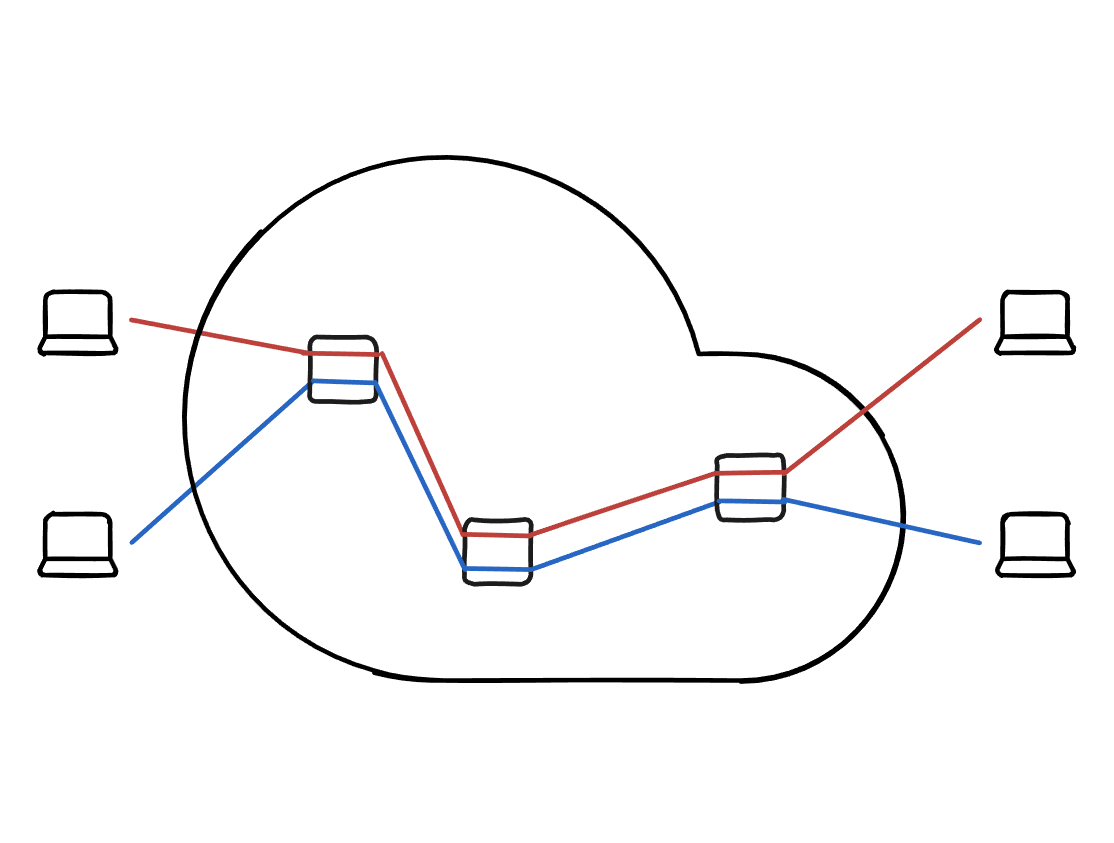
\includegraphics[width=0.95\textwidth]{comm-circuito}
  \caption{Commutazione di circuito}
\end{figure}

\noindent
Ogni canale è completamente dedicato alla comunicazione tra i 2 utenti, quindi
se più utenti vogliono comunicare tra di loro, bisogna riservare altre risorse.

\subsubsection{Vantaggi}
\begin{itemize}
  \item Risorse dedicate
  \item Ritardo deterministico

    \noindent
    \begin{itemize}
      \begin{figure}[H]
        \centering
        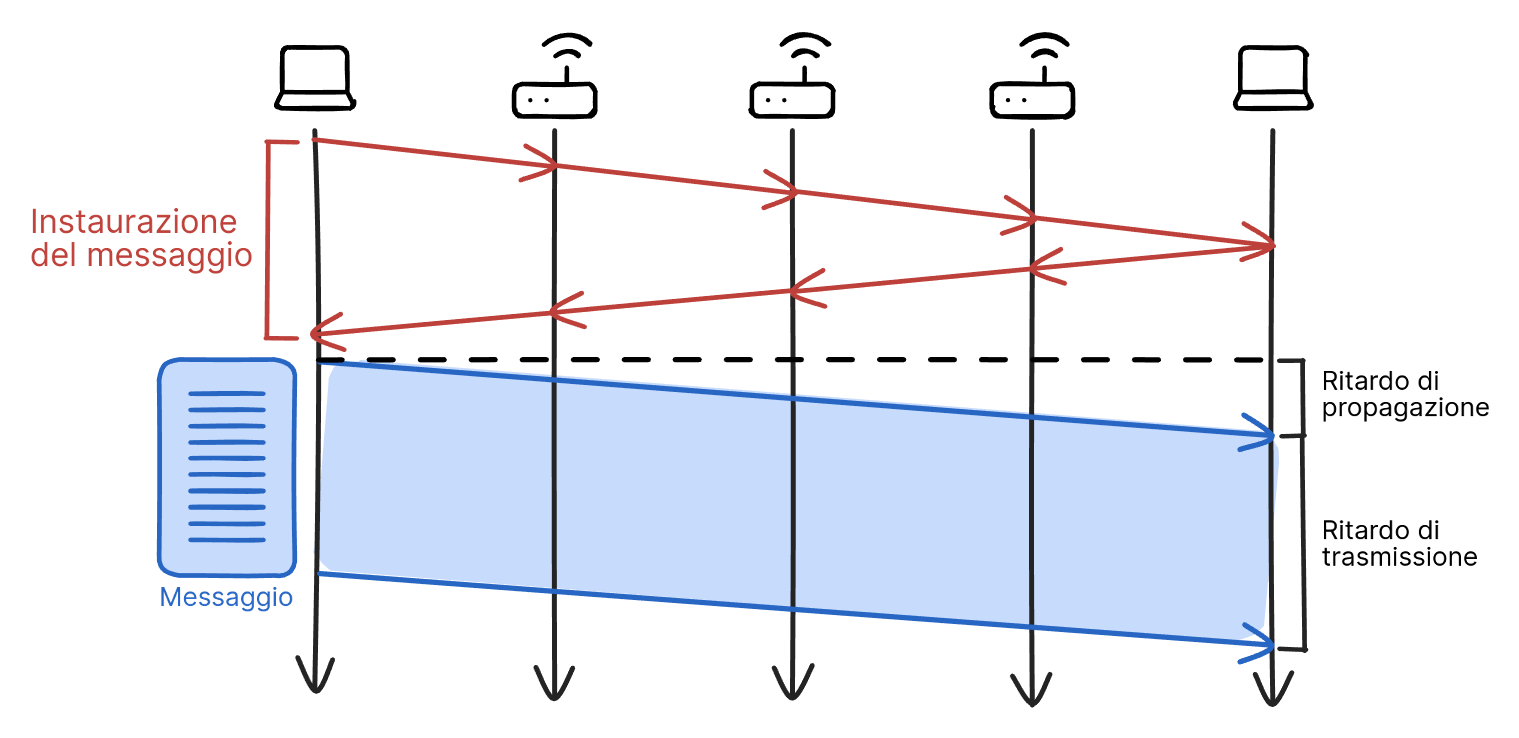
\includegraphics[width=0.95\textwidth]{ritardo}
        \caption{Ritardo}
      \end{figure}
      \item \textbf{Ritardo di trasmissione}: Tempo necessario per trasmettere il messaggio
      \item \textbf{Ritardo di propagazione}: Tempo necessario per trasmettere il messaggio
        da un nodo all'altro
    \end{itemize}
    Se il messaggio è grande \( L\,bit \) e il canale riservato è di \( B\,bit/s \),
    allora il tempo di trasmissione sarà:
    \[
    T = \frac{L}{B}
    \] 
    Il ritardo di trasmissione e di propagazione è deterministico, perchè
    dato il circuito di trasmissione, il tempo di trasmissione è noto.
\end{itemize}

\subsubsection{Svantaggi}
Nel corso di utilizzo sporadico si ha uno spreco di risorse, perchè il circuito
viene riservato per tutta la durata della comunicazione, anche se i 2 utenti
non stanno comunicando.
\begin{figure}[H]
  \centering
  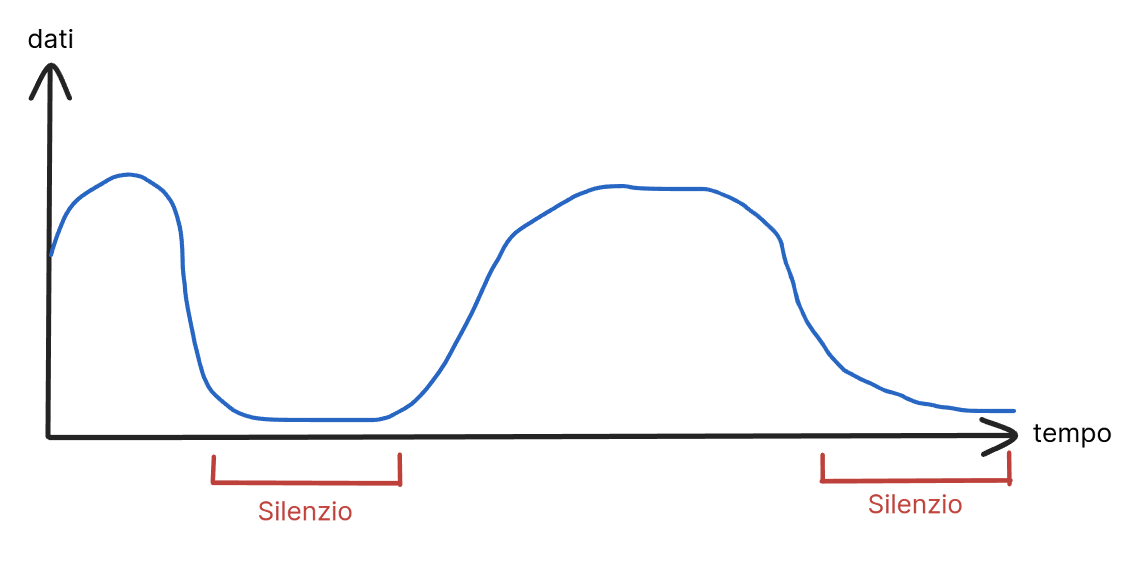
\includegraphics[width=0.70\textwidth]{silenzio}
  \caption{Spreco di risorse}
\end{figure}

\subsection{Reti a commutazione di pacchetto}
È la modalità di commutazione più utilizzata al giorno d'oggi.

\noindent
L'informazione (messaggio) viene suddivisa in \textbf{pacchetti} e ad ogni
pacchetto viene aggiunto un \textbf{header} per permettere:
\begin{itemize}
  \item La consegna del pacchetto stesso
  \item La ricostruzione del messaggio
\end{itemize}

Il messaggio è l'informazione da trasferire, mentre il pacchetto è una porzione
del messaggio stesso.

\noindent
Il messaggio prima della trasmissione viene separato in unità più piccole e a
queste unità viene aggiunta un'intestazione che serve a rendere le unità indipendenti
per poterle trasmettere in modo indipendente. L'intestazione permette la consegna del
pacchetto perchè contiene la destinazione del pacchetto e la ricostruzione del messaggio
perchè contiene il numero di sequenza del pacchetto.
\begin{figure}[H]
  \centering
  \begin{tikzpicture}
    \node[draw, minimum width=5cm, minimum height=1cm] at (0.45,0) (m) {Messaggio};
    \draw[->] (m.south) -- ++(0,-1);

    \coordinate (a) at (-2.7,-3);
    \draw (a) rectangle ++(1,1) node[midway] {$m_1$};
    \draw[blue,fill, fill opacity=0.1] (a) ++(0,1) rectangle ++(-0.5,-1);

    \coordinate (b) at (-0.8,-3);
    \draw (b) rectangle ++(1,1) node[midway] {$m_2$};
    \draw[blue,fill, fill opacity=0.1] (b) ++(0,1) rectangle ++(-0.5,-1);

    \coordinate (c) at (1.1,-3);
    \draw (c) rectangle ++(1,1) node[midway] {$m_3$};
    \draw[blue,fill, fill opacity=0.1] (c) ++(0,1) rectangle ++(-0.5,-1);

    \coordinate (d) at (2.9,-3);
    \draw (d) rectangle ++(1,1) node[midway] {$m_4$};
    \draw[blue,fill, fill opacity=0.1] (d) ++(0,1) rectangle ++(-0.5,-1);
    \draw[<-,blue] (d) ++(-0.25,1) -- ++(0,0.5) node[above,blue] {Header};

  \end{tikzpicture}
  \caption{Messaggio e pacchetti}
\end{figure}

\noindent I pacchetti vengono salvati all'interno di un \textbf{buffer}, cioè una
memoria temporanea, in attesa di essere trasmessi. Man mano che i pacchetti
vengono inviati vengono accumulati nel buffer dei router e questo avviene per
qualsiasi collegamento.
\begin{figure}[H]
  \centering
  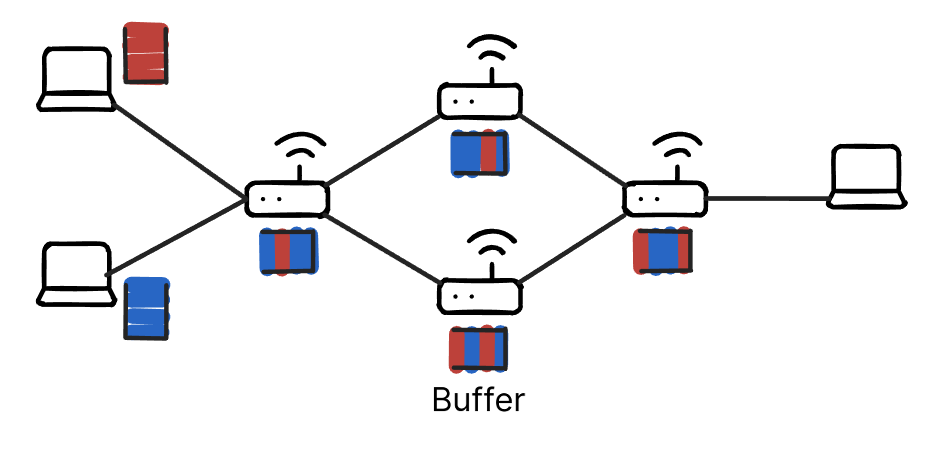
\includegraphics[width=0.95\textwidth]{buffer}
  \caption{Rappresentazione del buffer}
\end{figure}

\noindent
I pacchetti possono arrivare in ordine diverso rispetto a quello di trasmissione,
però grazie all'header è possibile ricostruire il messaggio originale.

\subsubsection{Vantaggi}
\begin{itemize}
  \item Utilizza le risorse solo quando ci sono pacchetti da trasmettere e questo
    viene chiamato \textbf{commutazione statistica}.
  \item \textbf{Multiplazione statistica}, cioè utilizzo lo stesso
    canale per trasmettere più pacchetti di utenti diversi.
\end{itemize}

\subsubsection{Svantaggi}
\begin{itemize}
  \item Potenziale perdita dei pacchetti: La memoria dei buffer ha una capacità finita,
    quindi se il tasso di ricezione dei pacchetti è superiore al tasso di
    smaltimento del buffer, esso inizia a riempirsi. Le perdite aumentano la
    complessità di gestione della rete.

  \item Ritardi aumentati

    \noindent
    I router prima di trasmettere i pacchetti, deve aspettare di ricevere tutti
    i pacchetti. Questo si chiama \textbf{store \& forward}. Di conseguenza
    più aumentano i router, più aumenta il ritardo di trasmissione.
    \begin{figure}[H]
      \centering
      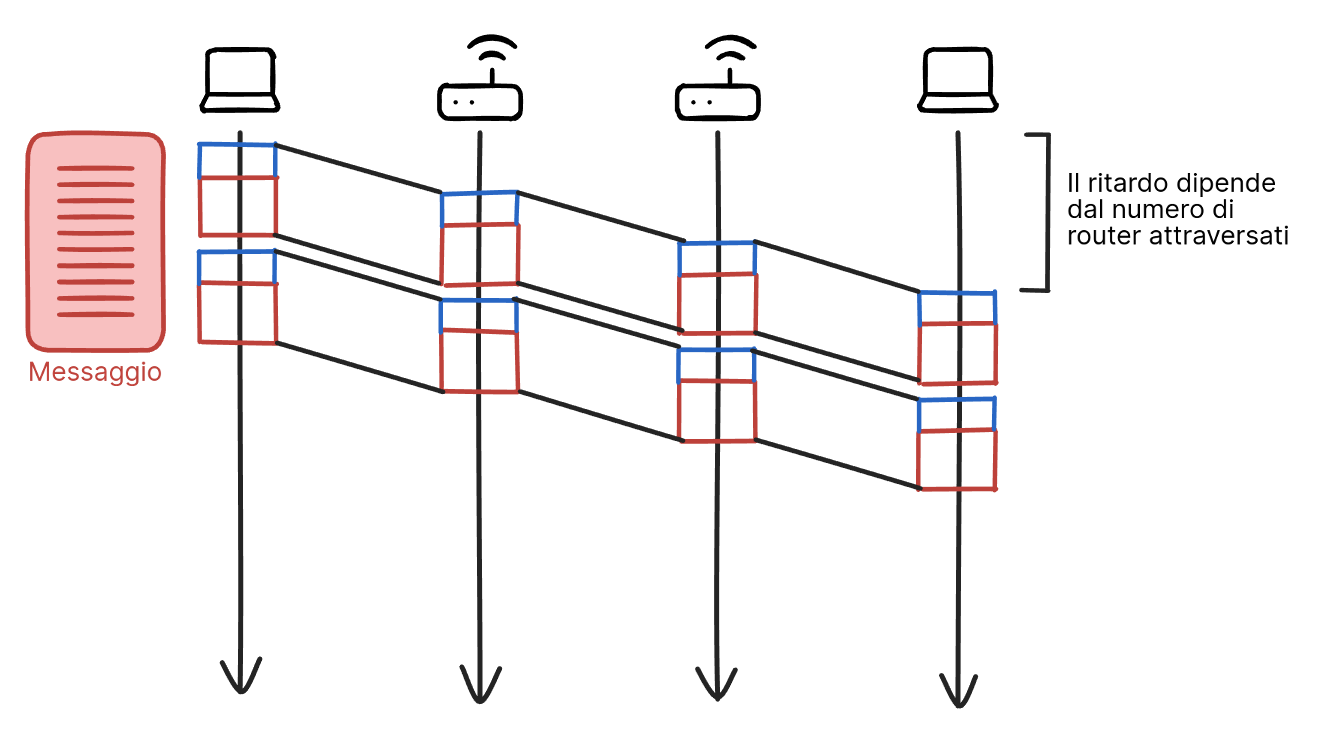
\includegraphics[width=0.95\textwidth]{ritardo-pacchetti}
      \caption{Ritardo di trasmissione dei pacchetti}
    \end{figure}
\end{itemize}

\section{Ritardi di trasmissione}
\begin{figure}[H]
  \centering
  \begin{tikzpicture}
    \draw (0,0) rectangle ++(3,3);
    \node[above] at (1.5,3) {Router};

    % Buffers
    \draw (2.3,2.8) -- ++(0.5,0) -- ++(0,-0.4) -- ++(-0.5,0) node[above left, scale=0.8]
      {Buffer};
    \draw (2.3,2.2) -- ++(0.5,0) -- ++(0,-0.4) -- ++(-0.5,0);
    \node at (2.6,1.6) {$\vdots$};
    \draw (2.3,1.17) -- ++(0.5,0) -- ++(0,-0.4) -- ++(-0.5,0);
    \draw (2.3,0.57) -- ++(0.5,0) -- ++(0,-0.4) -- ++(-0.5,0);

    % Inputs
    \draw (0,2.6) -- ++(-0.5,0);
    \draw (0,2.0) -- ++(-0.5,0);
    \node at (-0.25,1.6) {$\vdots$};
    \draw (0,1.0) -- ++(-0.5,0);
    \draw (0,0.4) -- ++(-0.5,0);

    \draw (-0.8,2.8) -- ++(-0.3,0) -- ++(0,-2.6) node[midway,left,align=center]
      {n° ingressi} -- ++(0.3,0);

    % Outputs
    \draw (3,2.6) -- ++(0.5,0);
    \draw (3,2.0) -- ++(0.5,0);
    \node at (3.25,1.6) {$\vdots$};
    \draw (3,1.0) -- ++(0.5,0);
    \draw (3,0.4) -- ++(0.5,0);

    \draw (3.8,2.8) -- ++(0.3,0) -- ++(0,-2.6) node[midway,right,align=center]
      {n° uscite} -- ++(-0.3,0);
  \end{tikzpicture}
  \caption{Struttura di un router}
\end{figure}

Su un singolo router le componenti principali del ritardo sono:
\begin{itemize}
  \item \textbf{Ritardo di elaborazione al nodo}: Tempo necessario per elaborare
    il pacchetto.
  \item \textbf{Ritardo di accodamento}: È il tempo speso nel buffer prima che
    il pacchetto venga trasmesso ed è la componente principale tra tutti i
    ritardi. (\( \frac{L}{B} \))
  \item \textbf{Ritardo di trasmissione}: Tempo necessario per trasmettere il
    pacchetto.
  \item \textbf{Ritardo di propagazione}: Tempo necessario per trasmettere il
    pacchetto da un nodo all'altro.
\end{itemize}

\subsection{Ordine di grandezza}
Dipende dalla distanza e dalla velocità di trasmissione del collegamento. La
distanza si distingue in:
\begin{itemize}
  \item \textbf{Locale}: \( < 10ms \) 
  \item \textbf{Internazionale}: \( 20-40ms \) 
  \item \textbf{Intercontinentale}: \( > 100ms \)
\end{itemize}

\subsection{Strumenti per calcolare il ritardo end-to-end}
\subsubsection{Ping}
Dati 2 utenti in 2 LAN diverse, il ping manda un pacchetto all'utente di destinazione
e l'utente che lo ha mandato prima o poi riceverà un messaggio di risposta (\textbf{
echo reply}). Il tempo che passa tra l'invio del pacchetto e la ricezione del
messaggio di risposta è il ritardo end-to-end.

\vspace{1em}
\noindent
Non si può sapere se il ritardo è asimmetrico o no, cioè se il ritardo di andata è uguale
al ritardo di ritorno, ma si può soltanto calcolare il ritardo totale.
\begin{figure}[H]
  \centering
  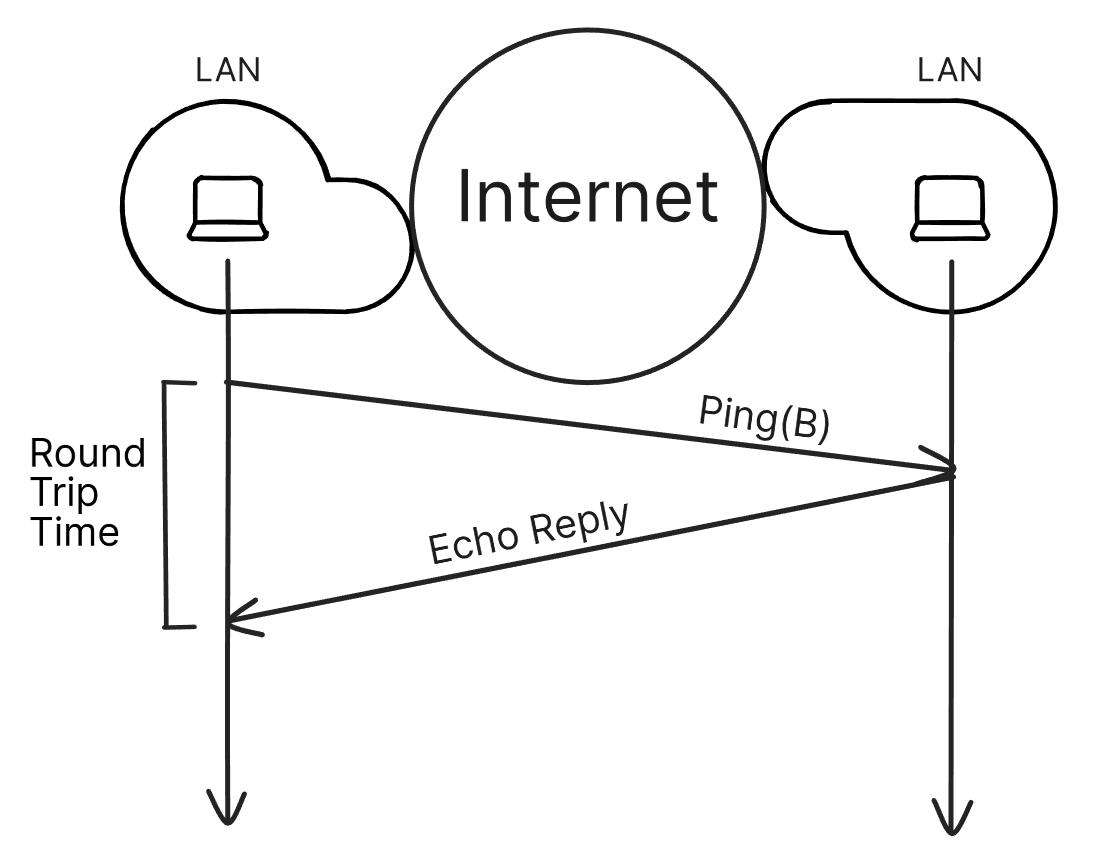
\includegraphics[width=0.70\textwidth]{ping}
  \caption{Ping}
\end{figure}

\noindent
Se si esegue il comando \texttt{ping} da un terminale si riceve il seguente output:
\begin{figure}[H]
  \centering
  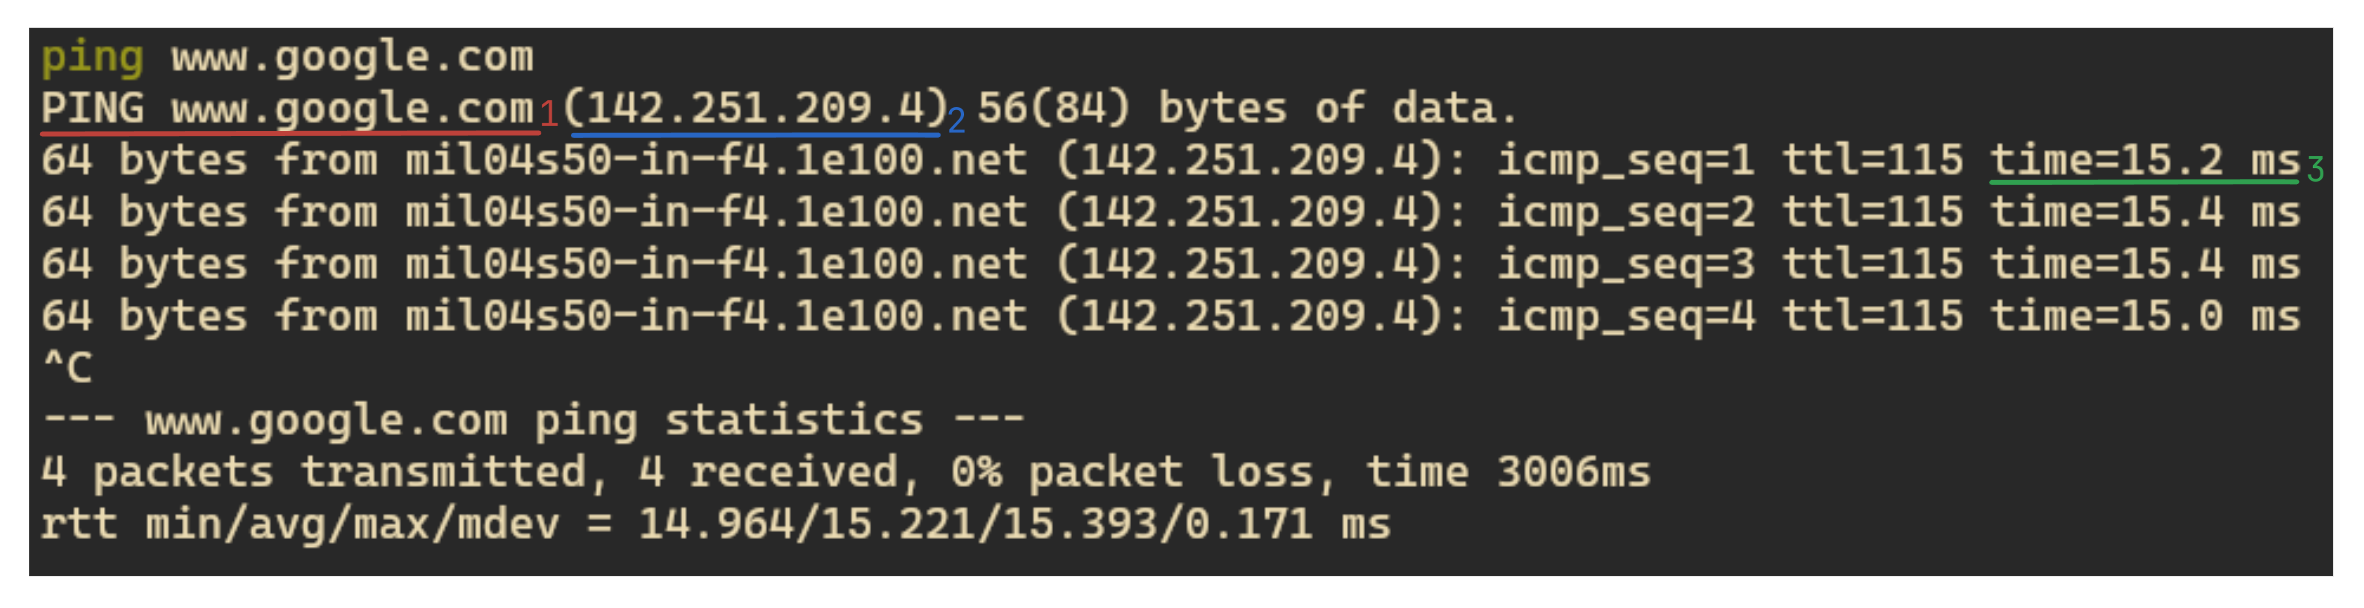
\includegraphics[width=1\textwidth]{ping-cmd}
  \caption{Output di ping}
\end{figure}

\begin{enumerate}
  \item Viene rieseguito il ping facendo riferimento al \textbf{server fisico}
  \item Tra parentesi viene rappresentato l'indirizzo che identifica il server, chiamato
    \textbf{indirizzo IP}
  \item Alla fine c'è il tempo di risposta del server
\end{enumerate}

\subsubsection{Traceroute}
Vengono mandati 3 messaggi al primo router e si calcolano i tempi di risposta tra
il primo utente e il primo router, poi viene fatta la stessa cosa con i seguenti
router fino ad arrivare all'utente di destinazione.
\begin{figure}[H]
  \centering
  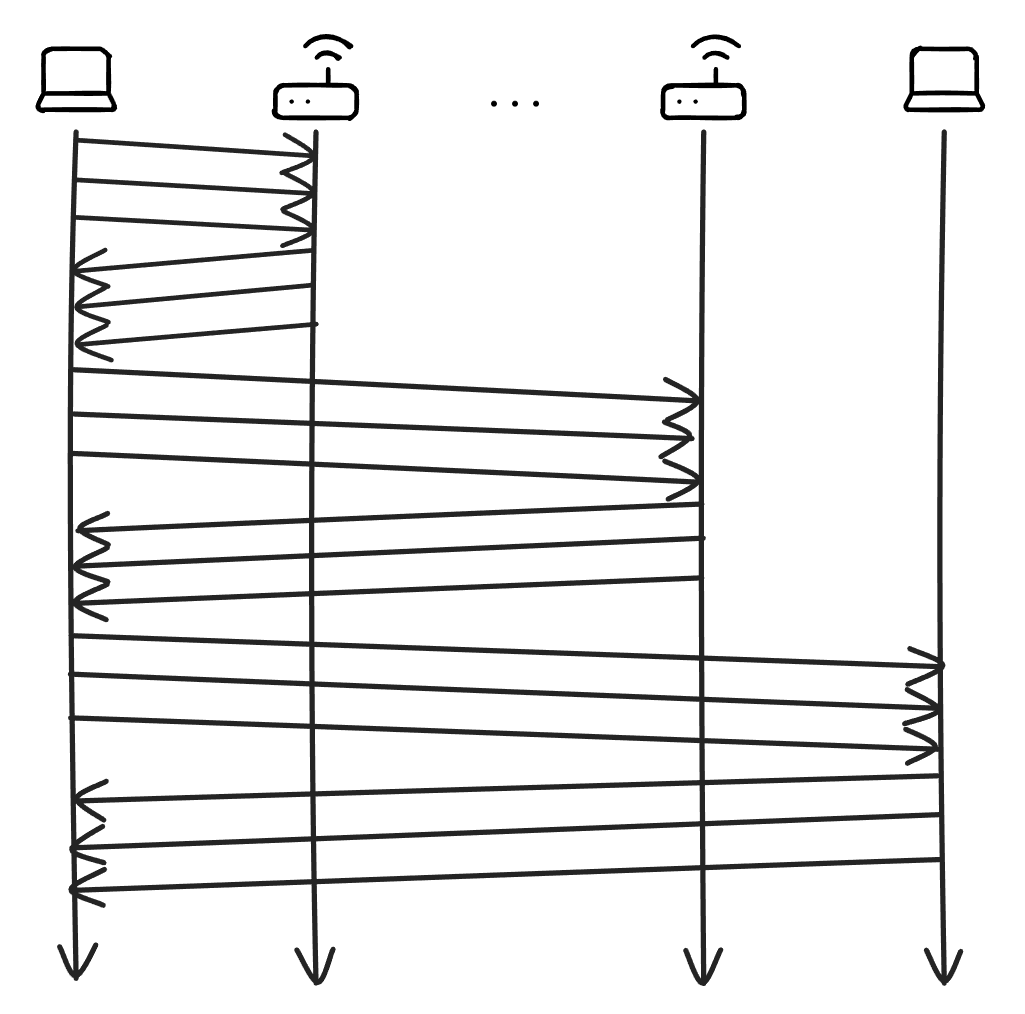
\includegraphics[width=0.70\textwidth]{traceroute}
  \caption{Traceroute}
\end{figure}

\noindent
Se si esegue il comando \texttt{traceroute} da un terminale si riceve il seguente output:
\begin{figure}[H]
  \centering
  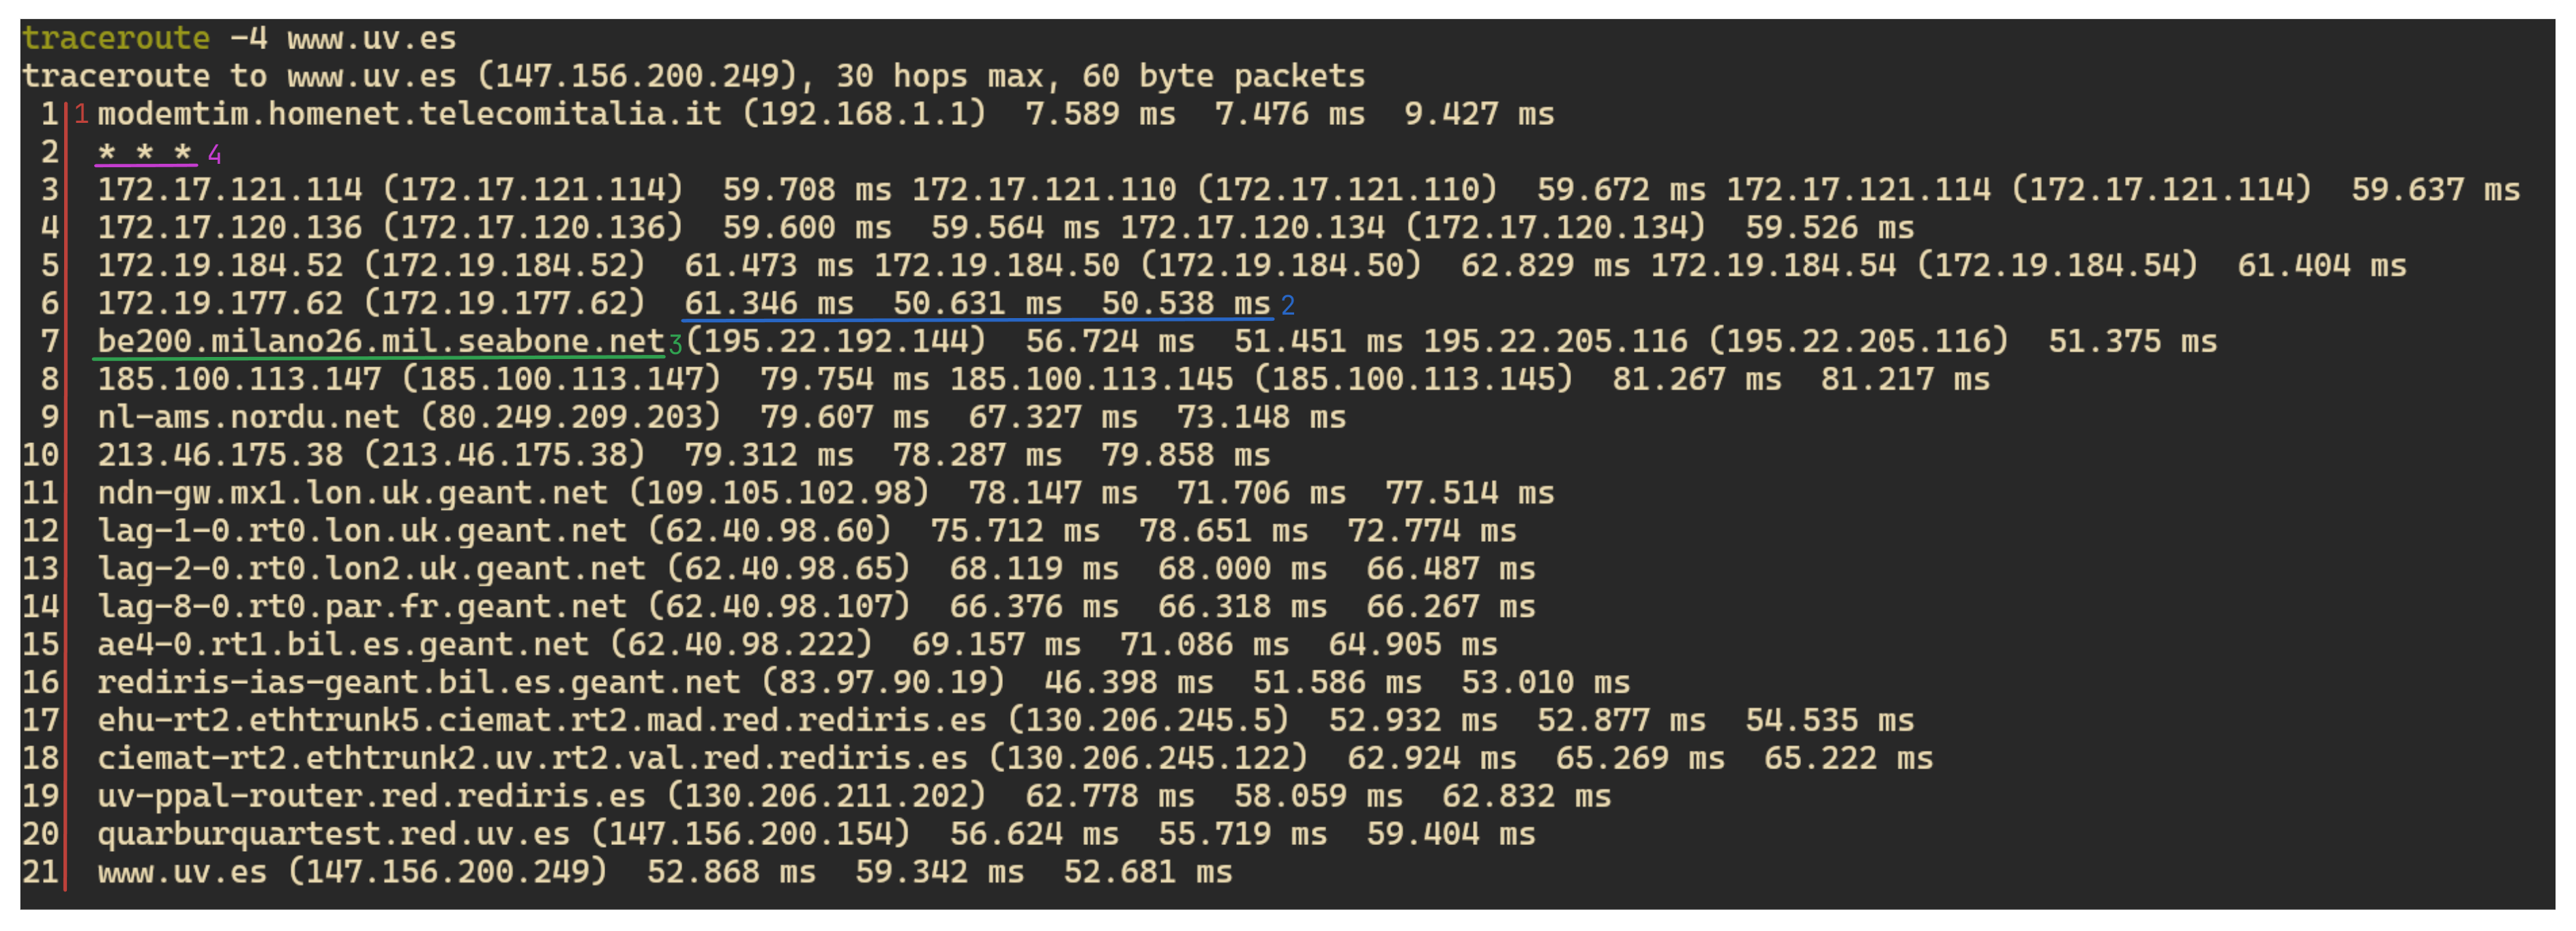
\includegraphics[width=1\textwidth]{traceroute-cmd}
  \caption{Output di traceroute}
\end{figure}

\begin{enumerate}
  \item Indica il numero di router attraversati
  \item Stampa i valori di ritardo dei 3 pacchetti trasmessi
  \item È il nome logico del router che si sta attraversando, da questo nome si può
    dedurre la posizione geografica del router e l'ISP a cui appartiene
  \item Gli asterischi indicano che il router è stato configurato in modo da ignorare
    i pacchetti e non mandare alcuna risposta, questo perchè serve soltanto a inoltrare
    i pacchetti ad un altro router.
\end{enumerate}


\subsection{Quantità di dati trasferiti}
La quantità di informazioni che si riesce a trasmettere si misura in \( \frac{bit}{s} \)
e questa informazione dipende dalla capacità di tutti i canali di trasmissione
attraversati.

\noindent
Ogni canale avrà una dimensione diversa e si può determinare la banda totale a
disposizione (\textbf{Throughput}) dal \textbf{collo di bottiglia}, cioè dalla minore
capacità di trasmissione tra tutti i canali attraversati.
\begin{figure}[H]
  \centering
  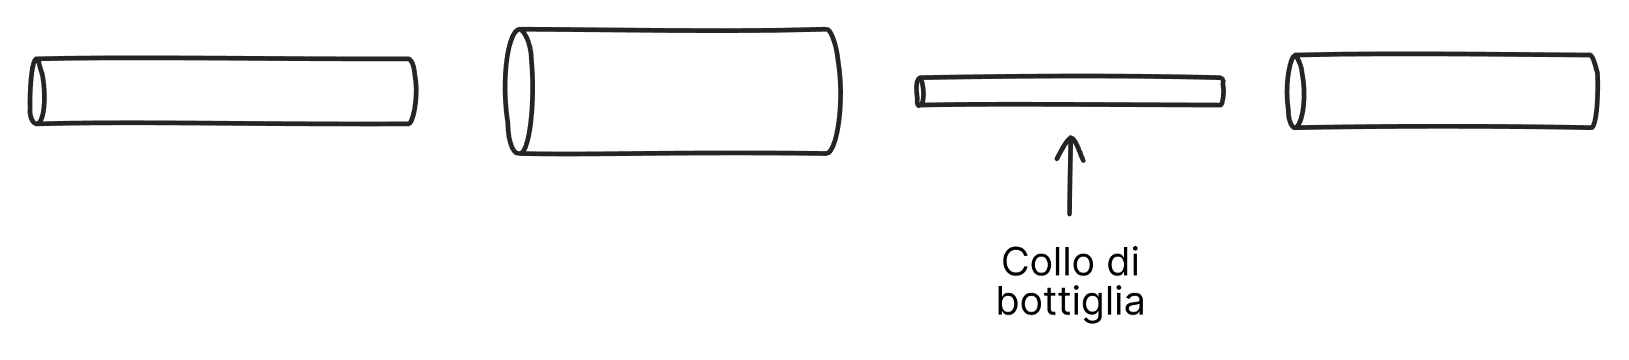
\includegraphics[width=0.70\textwidth]{throughput}
  \caption{Throughput}
\end{figure}

\section{Modello a strati}
Il modello a strati affronta la \textbf{comunicazione tra due entità} secondo la modalità
\textbf{divide et impera}.
\begin{figure}[H]
  \centering
  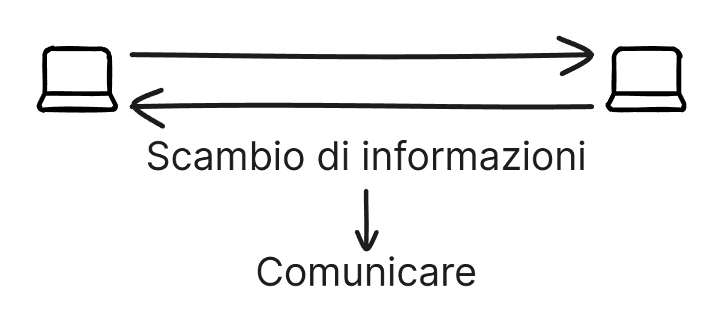
\includegraphics[width=0.70\textwidth]{comunicazione}
\end{figure}
\noindent
Per scambiare informazioni le due entità devono comunicare. La comunicazione si divide in:
\begin{itemize}
  \item \textbf{Comunicazione logica}: Gestisce le problematiche relative all'informazione

    \noindent Ad esempio:
    \begin{itemize}
      \item Linguaggio utilizzato
      \item Come comportarsi nello scambio
    \end{itemize}

  \item \textbf{Comunicazione Fisica}: Come trasferire i diversi bit. Il contenuto
    dell'informazione non è importante.
\end{itemize}

\begin{figure}[H]
  \centering
  \begin{tikzpicture}
    \draw (0,0) rectangle ++(3,-1) node[midway,draw] {Messaggio};
    \node[left,align=right,scale=0.7] at (0,-0.5)
      {Livello/Strato};

    \draw (0,-1) rectangle ++(3,-1);
    \node[blue,left,align=right,scale=0.7] at (0,-1.5)
      {Header specifico al livello\\Es: n° di sequenza};

    \draw (0,-2) rectangle ++(3,-1);
    \node[red,left,align=right,scale=0.7] at (0,-2.5)
      {Header specifico al livello\\Es: Indirizzo di destinazione};

    \draw (0,-3) rectangle ++(3,-1) node[midway] {$1101010010101001$};

    \coordinate (r1) at (0.4,-1.75);
    \draw[red] (r1) rectangle ++(0,0.5);
    \draw[blue] (r1) ++(0,0.5) rectangle ++(0.25,-0.5);
    \draw (r1) ++(0,0.5) ++(0.25,-0.5) rectangle ++(0.5,0.5) node[below right,yshift=-0.1cm] {$\ldots$};

    \coordinate[right of=r1, xshift=0.4cm] (r2);
    \draw[red] (r2) rectangle ++(0,0.5);
    \draw[blue] (r2) ++(0,0.5) rectangle ++(0.25,-0.5);
    \draw (r2) ++(0,0.5) ++(0.25,-0.5) rectangle ++(0.5,0.5);


    \coordinate (r3) at (0.18,-2.75);
    \draw[red] (r3) rectangle ++(0.25,0.5);
    \draw[blue] (r3) ++(0.25,0.5) rectangle ++(0.25,-0.5);
    \draw (r3) ++(0.25,0.5) ++(0.25,-0.5) rectangle ++(0.5,0.5) node[below right,yshift=-0.1cm] {$\ldots$};

    \coordinate[right of=r3, xshift=0.65cm] (r4);
    \draw[red] (r4) rectangle ++(0.25,0.5);
    \draw[blue] (r4) ++(0.25,0.5) rectangle ++(0.25,-0.5);
    \draw (r4) ++(0.25,0.5) ++(0.25,-0.5) rectangle ++(0.5,0.5);

    \draw[->] (3.2,0) -- ++(0,-3);



    \draw (5,0) rectangle ++(3,-1) node[midway,draw] {Messaggio};
    \draw (5,-1) rectangle ++(3,-1);
    \draw (5,-2) rectangle ++(3,-1);

    \draw (5,-3) rectangle ++(3,-1) node[midway] {$1101010010101001$};

    \coordinate (r1) at (5.4,-1.75);
    \draw[red] (r1) rectangle ++(0,0.5);
    \draw[blue] (r1) ++(0,0.5) rectangle ++(0.25,-0.5);
    \draw (r1) ++(0,0.5) ++(0.25,-0.5) rectangle ++(0.5,0.5) 
      node[below right,yshift=-0.1cm] {$\ldots$};

    \coordinate[right of=r1, xshift=0.4cm] (r2);
    \draw[red] (r2) rectangle ++(0,0.5);
    \draw[blue] (r2) ++(0,0.5) rectangle ++(0.25,-0.5);
    \draw (r2) ++(0,0.5) ++(0.25,-0.5) rectangle ++(0.5,0.5);


    \coordinate (r3) at (5.18,-2.75);
    \draw[red] (r3) rectangle ++(0.25,0.5);
    \draw[blue] (r3) ++(0.25,0.5) rectangle ++(0.25,-0.5);
    \draw (r3) ++(0.25,0.5) ++(0.25,-0.5) rectangle ++(0.5,0.5) 
      node[below right,yshift=-0.1cm] {$\ldots$};

    \coordinate[right of=r3, xshift=0.65cm] (r4);
    \draw[red] (r4) rectangle ++(0.25,0.5);
    \draw[blue] (r4) ++(0.25,0.5) rectangle ++(0.25,-0.5);
    \draw (r4) ++(0.25,0.5) ++(0.25,-0.5) rectangle ++(0.5,0.5);

    \draw[<-] (4.8,0) -- ++(0,-3);

    \draw[->,dashed] (3,-3.5) -- ++(2,0) node[midway,below,align=center,scale=0.8] {Trasmissione\\fisica};
  \end{tikzpicture}
  \caption{Comunicazione tra due entità}
\end{figure}
\noindent
Ad ogni \textbf{livello} (o strato) viene elaborata parzialmente l'informazione e
trasformata. Ogni livello aggiunge un \textbf{header} che contiene un'informazione
specifica a quel livello, seguendo un \textbf{protocollo} (specifico per quel livello).

\vspace{1em}
\noindent
Ogni livello ha uno o più protocolli associati, e l'insieme dei protocolli di tutti i
livelli è chiamato \textbf{stack protocollare}.

\subsection{Stack ISO/OSI}
Il modello \textbf{ISO/OSI} (International Standard Organization / Open System Interconnection)
definisce dei livelli a seconda del sistema:
\begin{itemize}
  \item \textbf{End system}:
    \begin{figure}[H]
      \centering
      \begin{tikzpicture}[scale=0.8]
        \draw (0,6) rectangle ++(3,1) node[midway] {Applicazione};
        \draw (0,5) rectangle ++(3,1) node[midway] {Presentazione};
        \draw (0,4) rectangle ++(3,1) node[midway] {Sessione};
        \draw (0,3) rectangle ++(3,1) node[midway] {Trasporto};
        \draw (0,2) rectangle ++(3,1) node[midway] {Rete};
        \draw (0,1) rectangle ++(3,1) node[midway,align=center] {Collegamento\\dati};
        \draw (0,0) rectangle ++(3,1) node[midway] {Fisico};
        \node[below] at (1.5,0) {End system};
      \end{tikzpicture}
      \caption{Stack ISO/OSI per l'end system}
    \end{figure}
  \item \textbf{Intermediate system}:
    \begin{figure}[H]
      \centering
      \begin{tikzpicture}[scale=0.8]
        \draw (0,2) rectangle ++(3,1) node[midway] {Rete};
        \draw (0,1) rectangle ++(3,1) node[midway,align=center] {Collegamento\\dati};
        \draw (0,0) rectangle ++(3,1) node[midway] {Fisico};
        \node[below] at (1.5,0) {Intermediate system};
      \end{tikzpicture}
      \caption{Stack ISO/OSI per l'intermediate system}
    \end{figure}
\end{itemize}

\subsection{Stack TCP/IP}
Nella pratica (rete Internet) si utilizza lo stack protocollare \textbf{TCP/IP}:
\begin{itemize}
  \item \textbf{End system}:
    \begin{figure}[H]
      \centering
      \begin{tikzpicture}[scale=0.8]
        \draw (0,4) rectangle ++(3,1) node[midway] {Applicazione};
        \draw (0,3) rectangle ++(3,1) node[midway] {Trasporto};
        \draw (0,2) rectangle ++(3,1) node[midway] {Rete};
        \draw (0,1) rectangle ++(3,1) node[midway,align=center] {Collegamento\\dati};
        \draw (0,0) rectangle ++(3,1) node[midway] {Fisico};
        \node[below] at (1.5,0) {End system};
      \end{tikzpicture}
      \caption{Stack TCP/IP per l'end system}
    \end{figure}
  \item \textbf{Intermediate system}:
    \begin{figure}[H]
      \centering
      \begin{tikzpicture}[scale=0.8]
        \draw (0,2) rectangle ++(3,1) node[midway] {Rete};
        \draw (0,1) rectangle ++(3,1) node[midway,align=center] {Collegamento\\dati};
        \draw (0,0) rectangle ++(3,1) node[midway] {Fisico};
        \node[below] at (1.5,0) {Intermediate system};
      \end{tikzpicture}
      \caption{Stack TCP/IP per l'intermediate system}
    \end{figure}
\end{itemize}

\noindent
Il nome deriva dai due principali protocolli utilizzati:
\begin{itemize}
  \item Protocollo di trasporto: \textbf{TCP} (Transport Control Protocol)
  \item Protocollo di rete: \textbf{IP} (Internet Protocol)
\end{itemize}

\subsection{Entità coinvolte nella comunicazione}
Su un calcolatore possono girare più applicazioni. Ogni applicazione
può avere una connessione attiva, quindi ci possono essere più connessioni
attive contemporaneamente.

\vspace{1em}
\noindent
Un applicazione può avere più istanze di comunicazione, cioè più connessioni
attive contemporaneamente.

\vspace{1em}
\noindent
Di conseguenza \textbf{l'istanza di un'applicazione} è la vera e propria entità
all'interno di una comunicazione. Quando si parla di entità si fa riferimento a uno
specifico processo che gira su un calcolatore

\subsubsection{Identificazione dei processi}
Per identificare un processo servono 2 informazioni:
\begin{enumerate}
  \item \textbf{Indirizzo IP}: Identifica il calcolatore
  \item \textbf{Porta}: Codice numerico che identifica il processo all'interno del 
    calcolatore
\end{enumerate}
\begin{figure}[H]
  \centering
  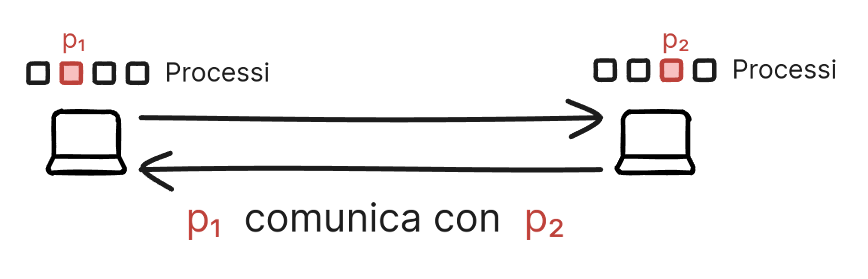
\includegraphics[width=0.7\textwidth]{comunicazione-processi}
  \caption{Comunicazione tra processi}
\end{figure}
Un flusso di comunicazione è identificato univocamente dalla tupla:
\[
  (IP_A, IP_B, Porta_A, Porta_B)
\]
La porta viene assegnata ad un processo soltanto quando esso inizia a comunicare.

\subsubsection{Ottenimento dell'IP e della porta}
Queste informazioni sono contenute negli header aggiunti ad ogni livello.
\begin{figure}[H]
  \centering
  \begin{tikzpicture}
    \node[draw, minimum width=5cm, minimum height=1cm] at (0.45,0) (m) {Messaggio};
    \draw[->] (m.south) -- ++(0,-1);

    \coordinate (a) at (-2.7,-3);
    \draw (a) rectangle ++(1,1) node[midway] {$m_1$};
    \draw[blue,fill, fill opacity=0.1] (a) ++(0,1) rectangle ++(-0.5,-1);

    \coordinate (b) at (-0.8,-3);
    \draw (b) rectangle ++(1,1) node[midway] {$m_2$};
    \draw[blue,fill, fill opacity=0.1] (b) ++(0,1) rectangle ++(-0.5,-1);

    \coordinate (c) at (1.1,-3);
    \draw (c) rectangle ++(1,1) node[midway] {$m_3$};
    \draw[blue,fill, fill opacity=0.1] (c) ++(0,1) rectangle ++(-0.5,-1);

    \coordinate (d) at (2.9,-3);
    \draw (d) rectangle ++(1,1) node[midway] {$m_4$};
    \draw[blue,fill, fill opacity=0.1] (d) ++(0,1) rectangle ++(-0.5,-1);
    \draw[<-,blue] (d) ++(-0.25,1) -- ++(0,0.5) node[above,blue] {Porta};
    \draw[blue] (d) ++(1.25,0.5) node[right,align=center] {Livello\\trasporto};

    \draw[->] (m.south) ++(0,-3) -- ++(0,-1);

    \coordinate (e) at (-3.7,-6);
    \draw (e) rectangle ++(1,1) node[midway] {$m_1$};
    \draw[blue,fill, fill opacity=0.1] (e) ++(0,1) rectangle ++(-0.5,-1);
    \draw[red,fill, fill opacity=0.1] (e) ++(-0.5,1) rectangle ++(-0.5,-1);

    \coordinate (f) at (-1.3,-6);
    \draw (f) rectangle ++(1,1) node[midway] {$m_2$};
    \draw[blue,fill, fill opacity=0.1] (f) ++(0,1) rectangle ++(-0.5,-1);
    \draw[red,fill, fill opacity=0.1] (f) ++(-0.5,1) rectangle ++(-0.5,-1);

    \coordinate (g) at (1.1,-6);
    \draw (g) rectangle ++(1,1) node[midway] {$m_3$};
    \draw[blue,fill, fill opacity=0.1] (g) ++(0,1) rectangle ++(-0.5,-1);
    \draw[red,fill, fill opacity=0.1] (g) ++(-0.5,1) rectangle ++(-0.5,-1);

    \coordinate (h) at (3.5,-6);
    \draw (h) rectangle ++(1,1) node[midway] {$m_4$};
    \draw[blue,fill, fill opacity=0.1] (h) ++(0,1) rectangle ++(-0.5,-1);
    \draw[red,fill, fill opacity=0.1] (h) ++(-0.5,1) rectangle ++(-0.5,-1);
    \draw[<-,red] (h) ++(-0.75,1) -- ++(0,0.5) node[above,red] {IP};
    \draw[red] (h) ++(1.25,0.5) node[right,align=center] {Livello\\di rete};

  \end{tikzpicture}
  \caption{Porta e IP}
\end{figure}

\noindent
Un pacchetto si può rappresentare nel seguente modo:
\begin{figure}[H]
  \centering
  \begin{tikzpicture}
    \draw[red] (0,0) rectangle ++(1,1);
    \node[red,above,scale=0.8,align=center] at (0.5,1) {Header\\livello\\di rete};

    \draw[dashed,blue] (0,0) ++(1.1,0.1) rectangle ++(0.8,0.8);
    \draw (0,0) ++(1,0) rectangle ++(4,1);

    \draw (0,0) ++(1,-0.2) -- ++(0,-0.2) -- ++(4,0) node[midway,below] {Payload}
      -- ++(0,0.2);
  \end{tikzpicture}
  \caption{Rappresentazione di un pacchetto}
\end{figure}
\noindent
oppure si può rappresentare anche come:
\begin{figure}[H]
  \centering
  \begin{tikzpicture}
    \draw[red] (0,0) rectangle ++(3,2) node[midway,above,align=center,scale=0.85,yshift=-0.5cm] {
        \texttt{01011100101101001}\\
        \texttt{01010011101101001}\\
        \texttt{10010110011010101}\\
      };
    \node[draw,red,scale=0.8,minimum width=3.5cm] at (1.5,0.3) {IP Destinazione};
    \node[draw,red,scale=0.8,minimum width=3.5cm] at (1.5,0.75) {IP Sorgente};

    \draw (0,0) rectangle ++(3,-3) node[midway,align=center,scale=0.9] 
      {
       \texttt{01011100101101001}\\
       \texttt{01010011101101001}\\
       \texttt{10010110011010101}\\
       \texttt{10101010110111010}\\
       \texttt{11101010100101000}\\
       \texttt{01010001110010110}\\
       \texttt{11101010110101100}
     };

   \draw[red] (3.1,0.1) -- ++(0.2,0) -- ++(0,0.85) node[midway,right,align=left] 
     {Dati sempre\\presenti} -- ++(-0.2,0);
  \end{tikzpicture}
\end{figure}

\section{Indirizzi IP}
Sono identificativi \textbf{univoci} di un'interfaccia di un host della rete Internet.
Un end system può avere soltanto un'interfaccia, ma un router deve avere minimo 2
interfacce per poter permettere la comunicazione tra più entità.


\begin{example}
  Un esempio di indirizzo IP è:
  \[
    1001 \; 1101 \;\; 0001 \; 1011 \;\; 0001 \; 0011 \;\; 0111 \; 1011
  \] 
  Per facilitare la lettura e la gestione degli indirizzi IP si usa la notazione
  \textbf{decimale puntata}. In questa notazione si considerano blocchi di 8 bit, di
  conseguenza si avranno 4 blocchi. Ogni blocco viene tradotto in un numero intero decimale
  compreso tra 0 e 255 e separato da un punto:
  \[
    157.27.19.123
  \] 
\end{example}

\subsection{Suddivisione dei bit}
I bit dell'indirizzo IP hanno tutti la stessa importanza?

\vspace{1em}
\noindent
Prendiamo ad esempio i numeri telefonici della rete fissa:
\[
  \underbrace{0039 \; 045 \; 802}_{\text{Prefisso}} \; \underbrace{7059}_{\text{Suffisso}}
\] 
\begin{itemize}
  \item Il prefisso è l'identificativo di una specifica organizzazione
  \item Il suffisso identifica un utente specifico all'interno dell'organizzazione
\end{itemize}

\vspace{1em}
\noindent
Allo stesso modo in un indirizzo IP si ha \textbf{prefisso} e \textbf{suffisso}
\begin{itemize}
  \item \textbf{Prefisso}: Identifica una rete specifica
  \item \textbf{Suffisso}: Identifica un'interfaccia di un host di una specifica rete 
\end{itemize}

\subsubsection{Identificazione del prefisso e del suffisso}
Nel caso dei numeri telefonici si inserisce una barra per separare il prefisso dal suffisso:
\[
  045/7021412
\]
Negli indirizzi IP il numero di bit dedicati al prefisso dipende dalla dimensione della
rete ed è indicato da una barra seguita da un numero.
\[
  157.27.19.123/16
\] 
Significa che i primi 16 bit dell'indirizzo IP sono dedicati al prefisso.
\[
  \underbrace{10011101 \;\; 00011011}_{n} \;\; \underbrace{00010011 \;\; 01111011}_{32 - n}
\] 
Quindi il numero di indirizzi si calcola come:
\[
  \text{indirizzi} = 2^{32-n}
\] 
\begin{example}
  \[
    n = 20 \to 2^{12} = 4096
  \] 
  \[
    n = 24 \to 2^8 = 256
  \] 
\end{example}

\noindent
Per identificare il numero di bit del prefisso i calcolatori utilizzano una sequenza di
32 bit in cui i bit associati al prefisso sono posti a \( 1 \) e gli altri a \( 0 \),
ad esempio:
\[
/16 \to 11111111 \;\; 11111111 \;\; 00000000 \;\; 00000000
\] 
Questa sequqnza è chiamata \textbf{maschera} perchè è abbinata all'indirizzo IP.
\begin{example}
\[
  \begin{aligned}
    \text{IP: } & \,10011101 \;\; 00011011 \;\;\, 00010011 \;\; 01111011\\
    \text{Mask: }& \underbrace{11111111 \;\; 11111111}_{\text{Prefisso}} \;\; \underbrace{00000000 \;\; 00000000}_{\text{Suffisso}}
  \end{aligned}
\] 
\end{example}
Facendo l'AND bit a bit tra l'IP e la maschera si ottiene l'indirizzo di rete a cui
quell'indirizzo IP appartiene.

\vspace{1em}
\noindent
La maschera può essere rappresentata anche in:
\begin{itemize}
  \item \textbf{Notazione decimale puntata}:
    \[
      /16 \to 255.255.0.0
    \] 
  \item \textbf{Notazione esadecimale}: si divide l'IP in gruppi da 4 bit e si convertono
    in esadecimale:
    \[
      /16 \to \texttt{0xffff0000}
    \] 
    Per capire che un numero è esadecimale, esso è prefissato da \texttt{0x}.
\end{itemize}

\subsection{Indirizzi IP riservati}
Non tutti gli indirizzi IP possono essere assegnati a degli host, infatti ce ne sono alcuni
riservati per delle funzioni specifiche:
\begin{enumerate}
  \item \textbf{This host}: È l'indirizzo IP del calcolatore stesso
    \[
      0.0.0.0
    \] 
  \item \textbf{Local broadcast} (o limited broadcast): Indirizzo IP che permette di 
    inviare un messaggio a tutti i calcolatori della rete locale
    \[
      255.255.255.255
    \]
  \item \textbf{Indirizzo di rete}: I primi \( n \) bit identificano una rete, gli altri
    \( 32 - n \) sono tutti posti a 0. Questo IP identifica la rete e nessun host può
    avere questo indirizzo
    \[
      \underbrace{1010100011}_{n} \underbrace{0000000000000000000000}_{32-n}
    \] 
  \item \textbf{Directed broadcast}: È un IP che permette di mandare un messaggio a tutti
    gli utenti di una rete specifica, anche esterna alla rete locale
    \[
      \underbrace{1010100011}_{n} \underbrace{1111111111111111111111}_{32-n}
    \] 
\end{enumerate}

\subsection{Conoscere il proprio indirizzo IP}
L'indirizzo ip e la dimensione del prefisso dipendono dalla rete a cui si è collegati.
Per conoscere il proprio indirizzo ip si usa il comando: \texttt{ifconfig}
\begin{figure}[H]
  \centering
  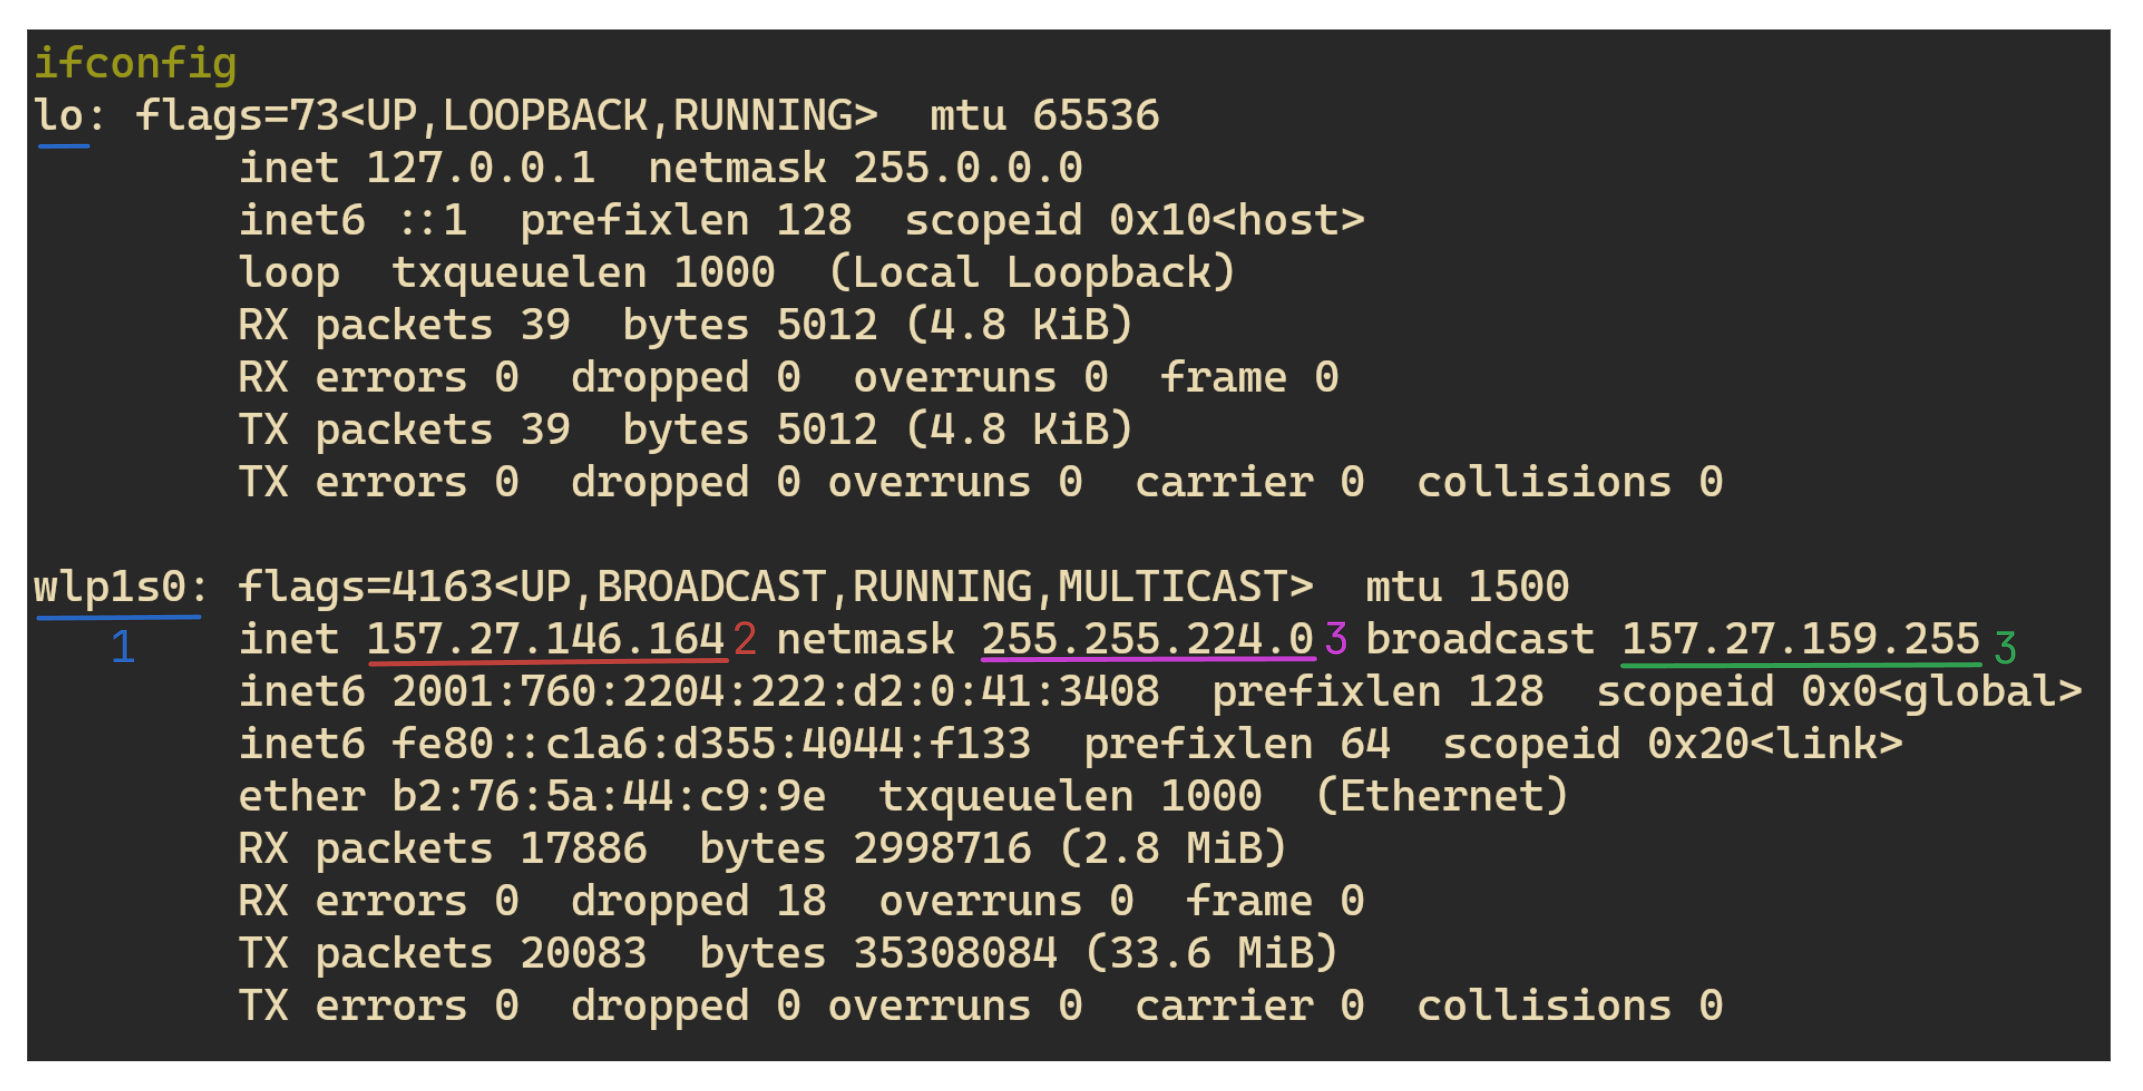
\includegraphics[width=1\textwidth]{ifconfig}
\end{figure}
\begin{enumerate}
  \item \textbf{Interfaccia di rete}: Rappresenta il collegamento tra il calcolatore e
    la rete.
  \item \textbf{Indirizzo ip}
  \item \textbf{Indirizzo broadcast}
  \item \textbf{Maschera}
\end{enumerate}

\vspace{1em}
\noindent
Altre informazioni sulla rete si possono ottenere con il comando: \texttt{whois}.
Questo comando si connette ad un server che contiene informazioni sugli indirizzi IP.

\noindent
L'output di questo comando da varie informazioni sull'IP messo come argomento, ma si
può notare che la maschera è diversa da quella che viene data in output dal comando
\texttt{ifconfig}.

\begin{itemize}
  \item Per \texttt{ifconfig} il prefisso è da 20 bit, quindi \( 2^{12} = 4096 \) indirizzi
  \item per \texttt{whois} il prefisso è da 16 bit, quindi \( 2^{16} = 65536 \) indirizzi
\end{itemize}

\noindent
Questo è dovuto al \textbf{subnetting}, cioè la creazione di sottoreti per partizionare
l'organizzazione distribuita sul territorio, quindi dei \( 65546 \) indirizzi, alcuni
verranno assegnati ad una sottorete e altri ad un'altra.
\begin{figure}[H]
  \centering
  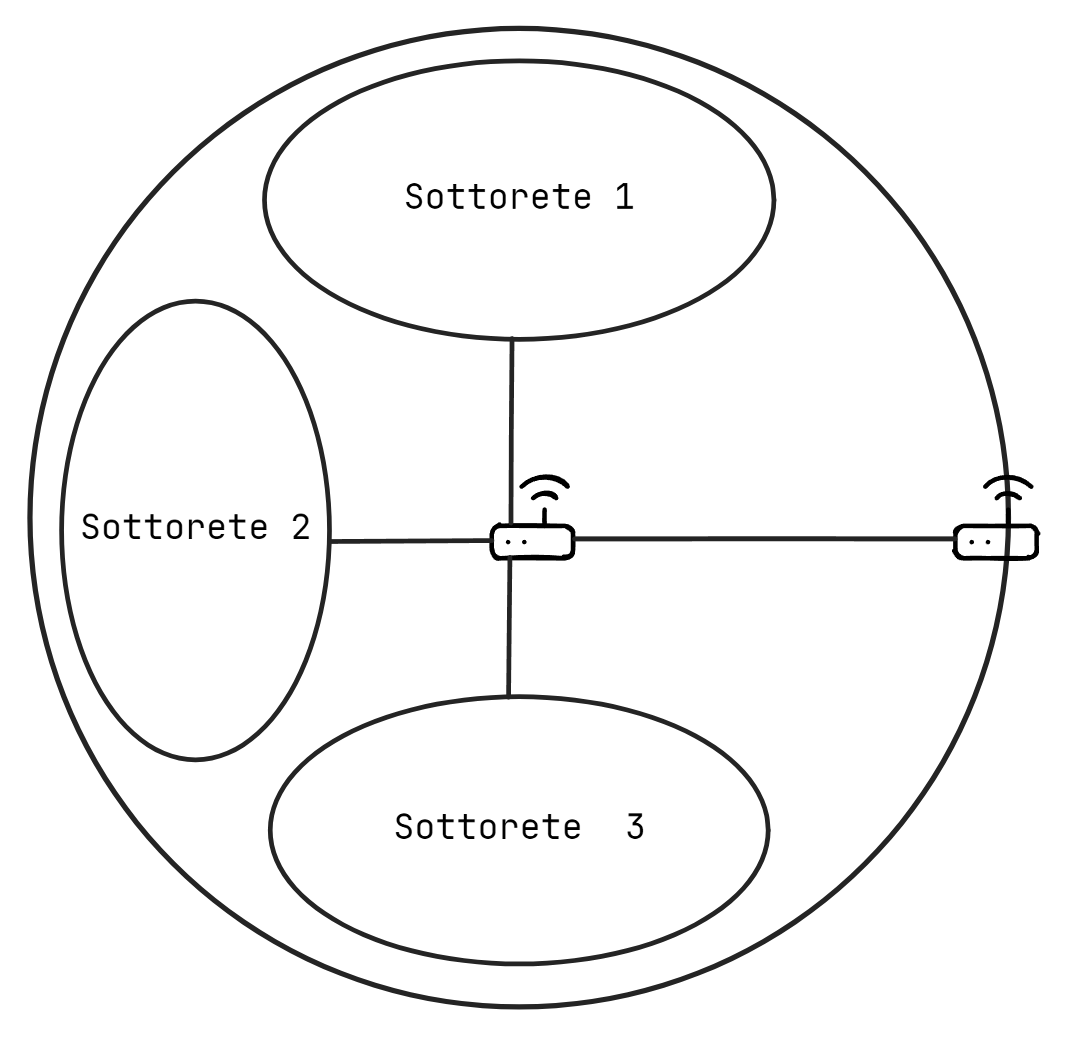
\includegraphics[width=0.70\textwidth]{subnetting}
  \caption{Subnetting}
\end{figure}
\noindent
Questa suddivisione dall'esterno non viene vista e questo è il motivo per cui ipconfig
mostra una maschera diversa da quella che si vede con il comando \texttt{whois}.

\subsection{Esercizi}
Conversione di IP decimale/binario
\begin{exercise}
  Dato il seguente IP:
  \[
    1110 \; 0111 \;\; 1101 \; 1011 \;\; 1000 \; 1011 \;\; 0110 \; 1111
  \] 
  la traduzione in decimale è la seguente:
  \[
    231.219.139.111
  \] 
\end{exercise}
\begin{exercise}
  Dato il seguente IP:
  \[
    221.34.255.82
  \] 
  la traduzione in binatio è la seguente:
  \[
    1101 \; 1101 \;\; 0010 \; 0010 \;\; 1111 \; 1111 \;\; 0101 \; 0010
  \] 
\end{exercise}

\subsection{Subnetting}
È il processo che permette di suddividere una rete in sottoreti.

\subsubsection{Creazione delle sottoreti partendo da un blocco di indirizzi assegnato}
Un'organizzazione richiede un blocco di indirizzi in base alle proprie necessità.
Prendendo come esempio l'Università di Verona, essa ha come indirizzo di rete il seguente:
\[
  157.27.0.0/16
\] 
si nota che i primi 16 bit sono dedicati al prefisso:
\[
  \underbrace{10011101 \;\; 00011011}_{\text{Prefisso}} \;\; \underbrace{00000000 \;\; 00000000}_{\text{Suffisso}}
\] 
Partendo da tale blocco si vogliono creare 2 sottoreti di pari dimensione. Per fare ciò
si può prendere il primo bit del suffisso, separarlo dal suffisso e associarlo al prefisso.
\[
  \underbrace{10011101 \;\; 00011011}_{\text{Prefisso}} \;\;
  \underbrace{0}_{\text{Sottorete}} \;\;
  \underbrace{0000000 \;\; 00000000}_{\text{Suffisso}}
\] 
Il bit assegnato al prefisso può avere 2 valori, quindi si possono creare 2 sottoreti:
\[
  \begin{aligned}
    \text{Sottorete 1: } &
    \underbrace{10011101 \;\; 00011011 \;\;\; 0}_{\text{Prefisso}} \;\;
    \underbrace{0000000 \;\; 00000000}_{\text{Suffisso}}\\
    \text{Sottorete 2: } &
    \underbrace{10011101 \;\; 00011011 \;\;\; 1}_{\text{Prefisso}} \;\;
    \underbrace{0000000 \;\; 00000000}_{\text{Suffisso}}
  \end{aligned}
\]
In notazione decimale puntata diventa:
\[
  \begin{aligned}
    \text{Sottorete 1: } &
    157.27.0.0/17\\
    \text{Sottorete 2: } &
    157.27.128.0/17
  \end{aligned}
\]
Quello che cambia è che il prefisso è diventato di 17 bit.

\vspace{1em}
\noindent
Da un blocco \( /16 \to 2^{32-16} = 65536 \) indirizzi si ottengono 2 blocchi
\( /17 \to 2^{32-17} = 2^{15} = 32768 \) indirizzi ciascuno.
\begin{figure}[H]
  \centering
  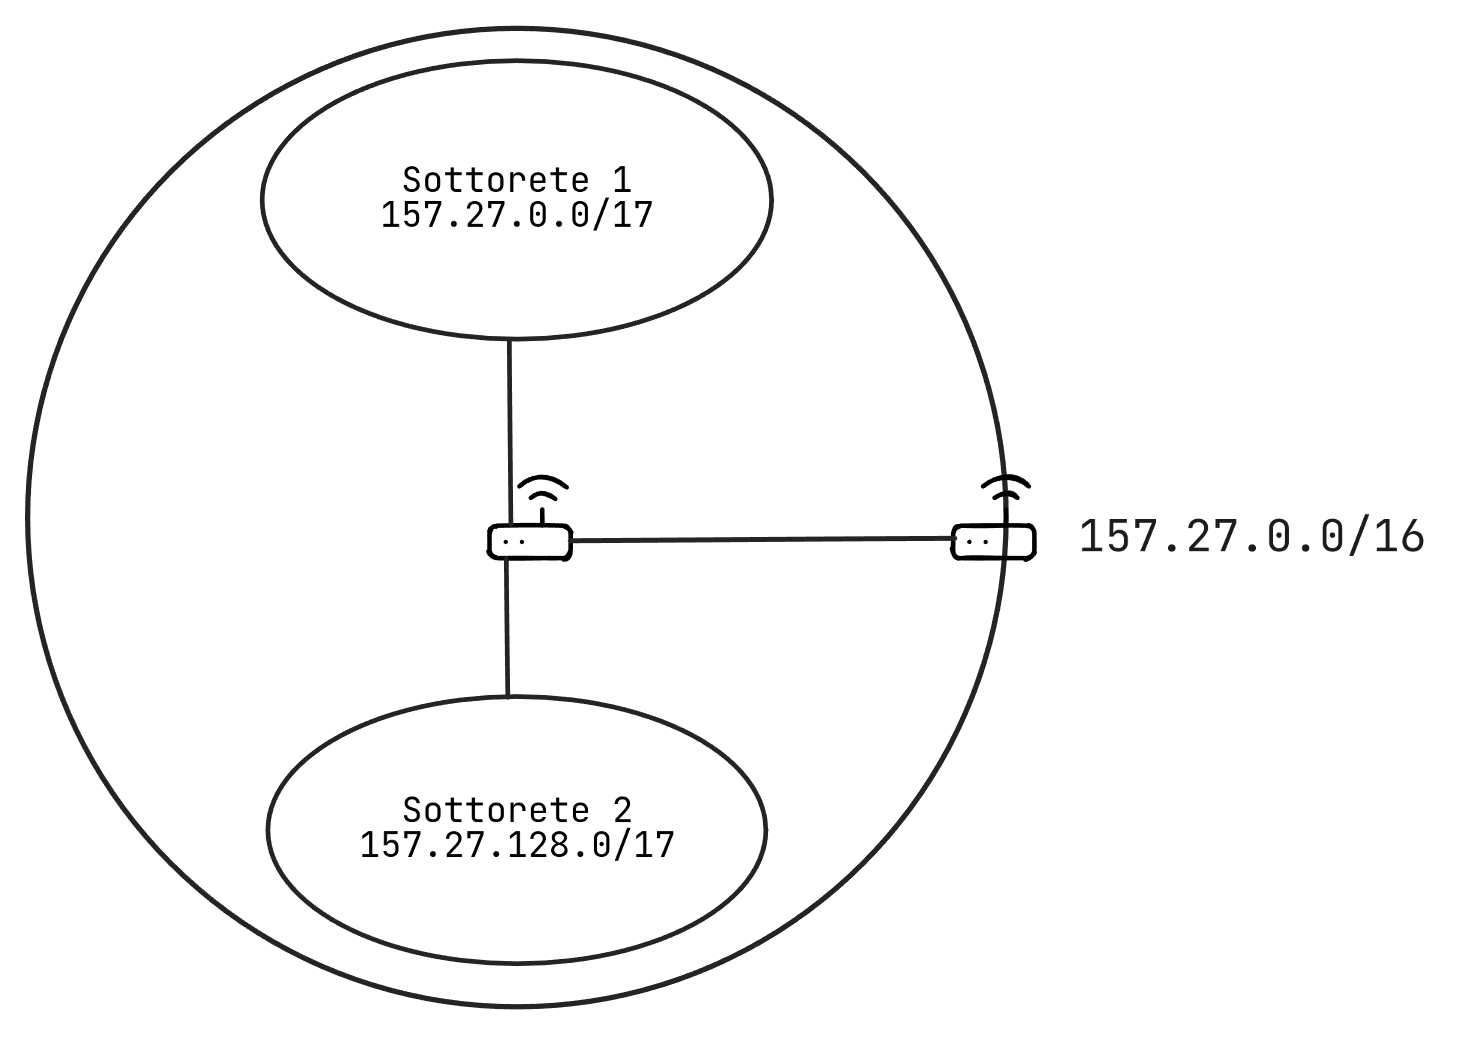
\includegraphics[width=0.70\textwidth]{esempio-subnetting}
  \caption{Risultato del subnetting}
\end{figure}

\noindent
I blocchi di indirizzi si chiamano \textbf{CIDR} (Classless Inter-Domain Routing).

\begin{itemize}
  \item \textbf{Nota storica}: In passato si usava la notazione \textbf{classful} in cui
    il numero di bit dedicati al prefisso era predererminato e venivano usati i bit
    iniziali per distinguere i diversi casi. Ad esempio:
    \begin{itemize}
      \item \textbf{Classe A}: 8 bit di prefisso se l'IP iniziava con 0:
        \[
          \underbrace{0 \;\;\; 1010010}_{\text{Prefisso}} \;\; \underbrace{00000000 \;\; 00000000 \;\; 00000000}_{\text{Suffisso}}
        \] 
      \item \textbf{Classe B}: 16 bit di prefisso se l'IP iniziava con 10:
        \[
          \underbrace{10 \;\;\; 010010 \;\; 10110100}_{\text{Prefisso}} \;\; \underbrace{00000000 \;\; 00000000}_{\text{Suffisso}}
        \]
      \item \textbf{Classe C}: 24 bit di prefisso se l'IP iniziava con 110:
        \[
          \underbrace{110 \;\;\; 010010 \;\; 10110100 \;\; 00000000}_{\text{Prefisso}} \;\; \underbrace{00000000}_{\text{Suffisso}}
        \]
    \end{itemize}
    L'informazione del prefisso era codificata nell'indirizzo stesso e quindi non c'era
    bisogno di aggiungere un'informazione all'IP come ad esempio la maschera.

    Per l'alta richiesta di indirizzi, l'indirizzamento classful non era sufficiente:
    \begin{table}[H]
      \centering
      \begin{tabular}{c|c|c}
        Classe & N° reti              & N° host              \\
        \hline
             A & $2^{7} \approx 16K$  & $2^{24} \approx 16M$ \\
             B & $2^{14} \approx 16K$ & $2^{16} \approx 65K$ \\
             C & $2^{21} \approx 2M$  & $2^{8} \approx 256$  \\
      \end{tabular}
    \end{table}
    \noindent
    Si esaurirono presto le classi A e B, quindi si passò al CIDR.
\end{itemize}

\vspace{1em}
\noindent
A volte assegnare delle sottoreti di uguale dimensione è uno spreco perchè certe esigenze
richiedono meno indirizzi e altre di più, quindi si dovrebbe suddividere la rete in sottoreti 
di dimensione \textbf{diversa}.

\section{Livello applicativo}
Il livello applicativo è il livello più alto dello stack protocollare:
\begin{figure}[H]
  \centering
  \begin{tikzpicture}[scale=0.8]
    \draw[fill,blue,fill opacity=0.2,text=black,text opacity=1] (0,4) rectangle ++(3,1) node[midway] {Applicazione};
    \draw (0,3) rectangle ++(3,1) node[midway] {Trasporto};
    \draw (0,2) rectangle ++(3,1) node[midway] {Rete};
    \draw (0,1) rectangle ++(3,1) node[midway,align=center] {Collegamento\\dati};
    \draw (0,0) rectangle ++(3,1) node[midway] {Fisico};
  \end{tikzpicture}
  \caption{Stack TCP/IP}
\end{figure}

\noindent
Questo livello genera un messaggio che può essere di tipo diverso, ad esempio:
\begin{itemize}
  \item Richiesta HTTP
  \item Risposta HTTP
  \item Email
  \item Il frame di un video
\end{itemize}
Quando un messaggio viene generato da un'applicazione si deve decidere quale protocollo
utilizzare a livello di trasporto:
\begin{itemize}
  \item \textbf{TCP} (Transmission Control Protocol): È un protocollo orientato
    alla connessione (\textbf{Connection oriented}) e affidabile. Questo protocollo da
    la garanzia che il messaggio arrivi a destinazione.
  \item \textbf{UDP} (User Datagram Protocol): È un protocollo non orientato alla
    connessione (\textbf{Connectionless}) e non affidabile. Questo protocollo non da la
    garanzia che il messaggio arrivi a destinazione e quindi non è detto che il messaggio
    arrivi.
\end{itemize}

\noindent
Un servizio di trasporto \textbf{affidabile} garantisce che la consegna arrivi a destinazione.

\subsection{Esempi di applicazioni e relativi protocolli di trasporto}
\begin{itemize}
  \item \textbf{Web}:
  Un esempio di applicazione è il browser web che utilizza il protocollo \texttt{HTTP}
  per trasferire dati attraverso la rete. Quando si consegnano testo e immagini
  non si devono commettere errori, quindi in questi casi il protocollo \texttt{HTTP}
  si appoggia a TCP.

  \item \textbf{Posta elettronica}:
  Un'altro esempio è la posta elettronica che utilizza il protocollo \texttt{SMTP}
  per inviare la posta. Questo protocollo richiede un servizio affidabile, quindi
  se un pacchetto viene perso, il protocollo TCP si preoccupa di recuperarlo.

  \item \textbf{Audio/video}:
  Per la trasmissione di audio e video di solito i protocolli sono proprietari, ma in
  questo caso non è necessaria l'affidabilità, basta garantire la tolleranza alle
  perdite, quindi ci si appoggia al protocollo UDP.

  \item \textbf{DNS}:
  Per navigare su internet si usa il protocollo \textbf{DNS} (Domain Name System)
  che è il servizio che traduce i nomi logici nei corrispettivi indirizzi ip.
\end{itemize}

\subsection{Socket}
Quando un'applicazione deve mandare un messaggio ad un'altra applicazione essa apre
un \textbf{socket} verso la destinazione. Un socket è un'interfaccia di comunicazione 
(astrazione software) che identifica un flusso informativo bidirezionale. Per aprire un
socket bisogna specificare:
\begin{itemize}
  \item Protocollo di trasporto
  \item Indirizzo IP di destinazione
  \item Indirizzo IP sorgente
  \item Porta di destinazione
  \item Porta di sorgente
\end{itemize}
L'apertura di un socket è effettuata soltanto da uno dei due processi.
\begin{figure}[H]
  \centering
  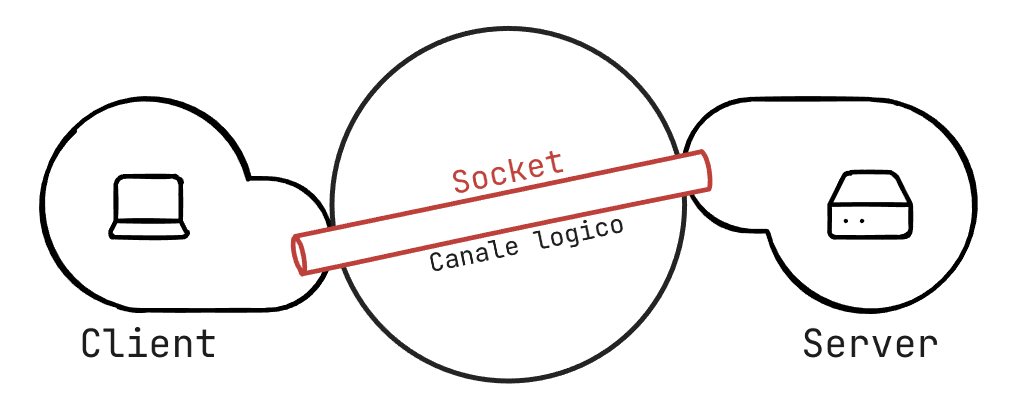
\includegraphics[width=0.7\textwidth]{socket}
\end{figure}

\noindent
Tra i due processi comunicanti si possono identificare due ruoli distinti:
\begin{enumerate}
  \item \textbf{Processo Client}: È il processo che è responsabile dell'inizio della
    comunicazione. Il client ha un indirizzo IP dinamico, cioè cambia in base alla
    rete a cui è collegato.

  \item \textbf{Processo Server}: È il processo che sta su un host sempre raggiungibile
    e sempre in ascolto. Il server ha un indirizzo IP statico.
\end{enumerate}

\subsection{Protocolli web}
\subsubsection{Protocollo HTTP}
Il protocollo \textbf{HTTP} (HyperText Transfer Protocol) è un protocollo di livello
applicativo usato per la trasmissione di documenti ipertestuali. Questo protocollo
è di tipo \textbf{testuale} (i messaggi sono scritti in ASCII),
determina il formato dei messaggi ed è basato sul modello \textbf{richiesta/risposta}:
\begin{itemize}
  \item \textbf{Richiesta}: Il client apre un socket, invia un messaggio di richiesta
    al server e aspetta la risposta.
  \item \textbf{Risposta}: Il server deve inviare un messaggio di risposta alla richiesta 
    del client
\end{itemize}
Se la richiesta non fosse ben formata il server risponde con un messaggio di errore.
Per cui il protocollo prevede sempre, ad ogni richiesta, che ci sia una risposta, positiva
o negativa.

Il server contiene delle pagine web, con eventualmente altri contenuti ad esempio immagini.
Il file di testo principale (\texttt{index.html}).
\begin{figure}[H]
  \centering
  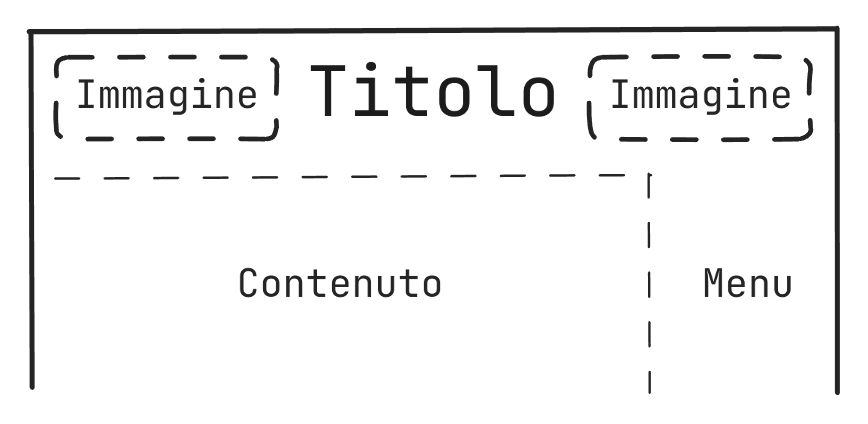
\includegraphics[width=0.7\textwidth]{html}
\end{figure}
\noindent
Un file \texttt{html} definisce sia la struttura che il contenuto di una pagina web.
\begin{figure}[H]
  \centering
  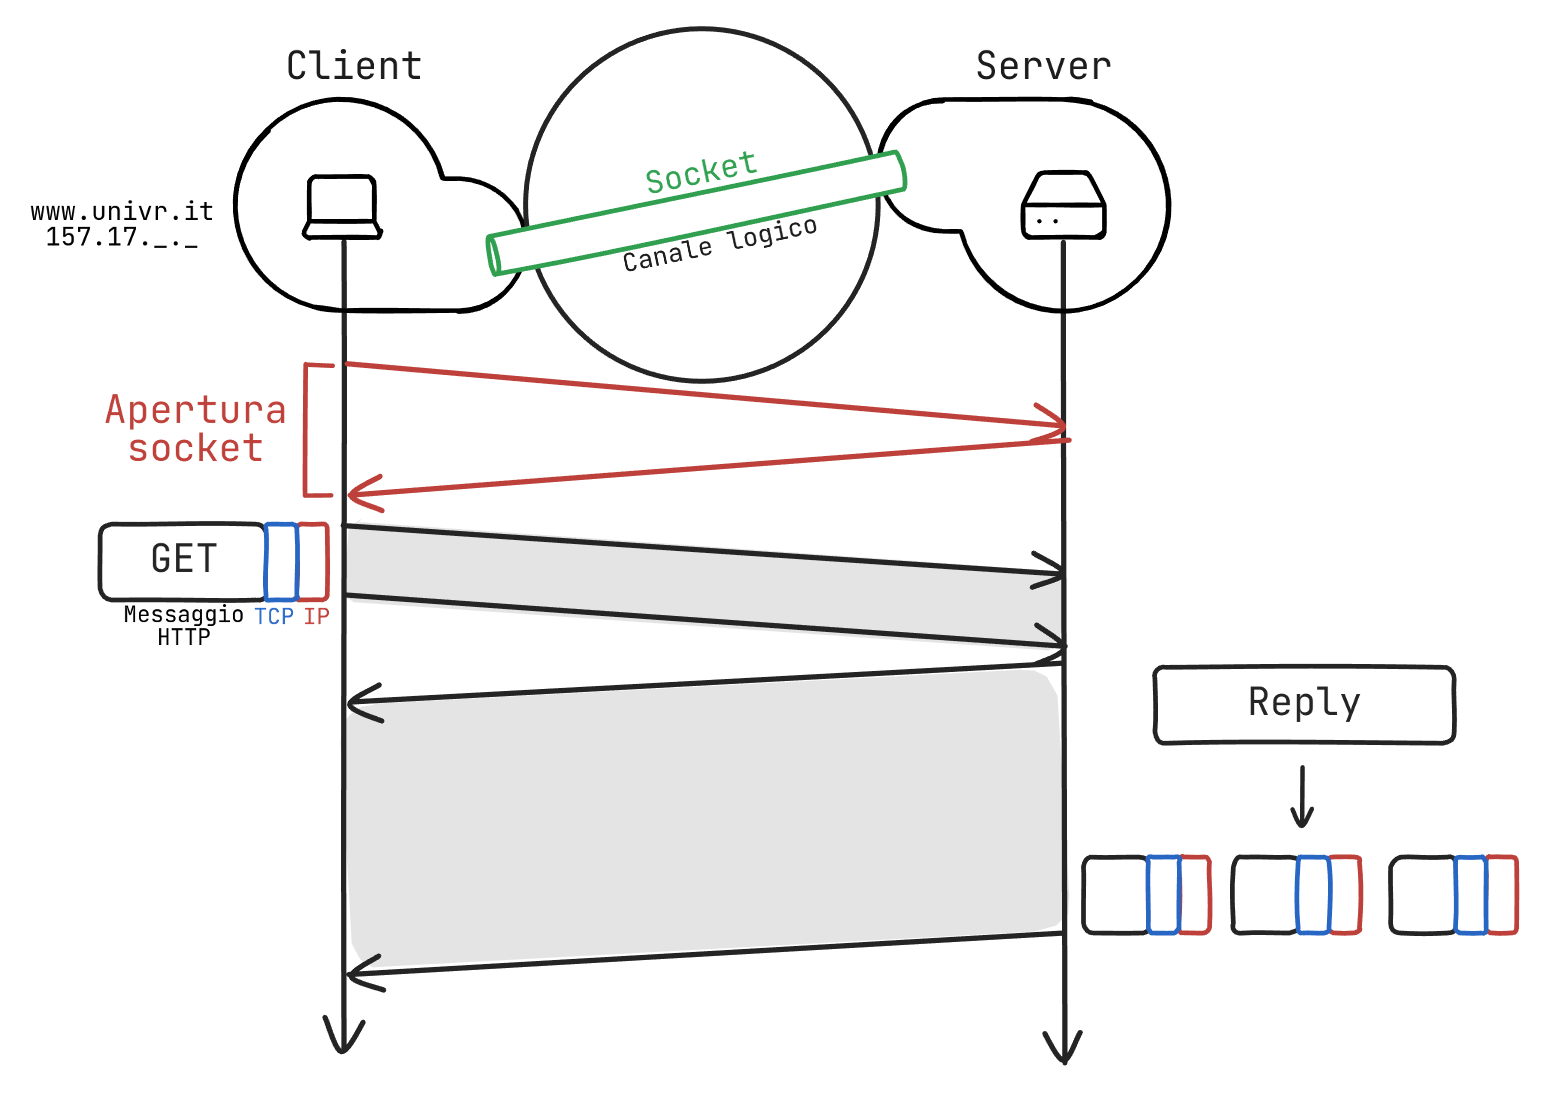
\includegraphics[width=0.9\textwidth]{comunicazione-socket}
\end{figure}

\vspace{1em}
\noindent
La struttura delle richieste HTTP è la seguente:
\begin{enumerate}
  \item Riga di richiesta
  \item Una o più righe di intestazione
\end{enumerate}

\begin{example}
  Un'esempio di richiesta HTTP è:
  \begin{lstlisting}[language=Scala]
    GET /index.html HTTP/1.1 // -- Riga di richiesta
    Host: www.univr.it       // -- Riga di intestazione
    User-Agent: Mozilla/5.0  // (intestazione facoltativa)
    Accept-language: en      // (intestazione facoltativo)
  \end{lstlisting}
  che corrisponde a una richiesta di una pagina web del seguente tipo:
  \[
    \underbrace{\texttt{www.univr.it}}_{\text{Server}} 
      \underbrace{\texttt{/index.html}}_{\text{File richiesto}}
  \]
  \label{http-request}
\end{example}

\noindent
Per fare una richiesta si utilizzano dei \textbf{metodi}:
\begin{itemize}
  \item \texttt{GET}: Richiede una rappresentazione di una risorsa specifica
  \item \texttt{POST}: Invia informazioni al server
  \item \texttt{HEAD}: Richiede una risposta identica a quella di una richiesta \texttt{GET}
    ma senza il corpo del messaggio, quindi solo con le intestazioni
  \item \texttt{PUT}: Carica una rappresentazione di una risorsa specifica
  \item \texttt{DELETE}: Cancella la risorsa specificata
\end{itemize}

\vspace{1em}
\noindent
La struttura delle risposte HTTP è la seguente:
\begin{enumerate}
  \item Riga di stato:
    \begin{itemize}
      \item Versione del protocollo
      \item Codice di stato
      \item Messaggio di stato
    \end{itemize}
  \item Una o più righe di intestazione
  \item Il corpo del messaggio
\end{enumerate}

\begin{example}
  Un'esempio di risposta HTTP è:
  \begin{lstlisting}[language=Scala]
    HTTP/1.1 200 OK          // -- Riga di stato
    Date: Mon, 23 May 2005   // -- 
    Content-Type: text/html  //  | Righe di intestazione
    Content-Length: 122      // -- 
                             // Riga vuota obbligatoria~~~
    <html>...</html>         // -- Corpo del messaggio
  \end{lstlisting}
\end{example}

\noindent
Per inviare e ricevere messaggi HTTP si può usare il comando \texttt{nc} o \texttt{netcat}
e scrivere una richiesta HTTP come mostrato nell'esempio \ref{http-request}.

\vspace{1em}
\noindent
Altri elementi del protocollo HTTP che possono estendere il funzionamento sono i \textbf{
cookies}. I cookies sono un meccanismo utilizzato dai server web per capire se è già
avvenuta un'interazione con un determinato client in passato. L'IP non basta perchè
è dinamico.
\begin{figure}[H]
  \centering
  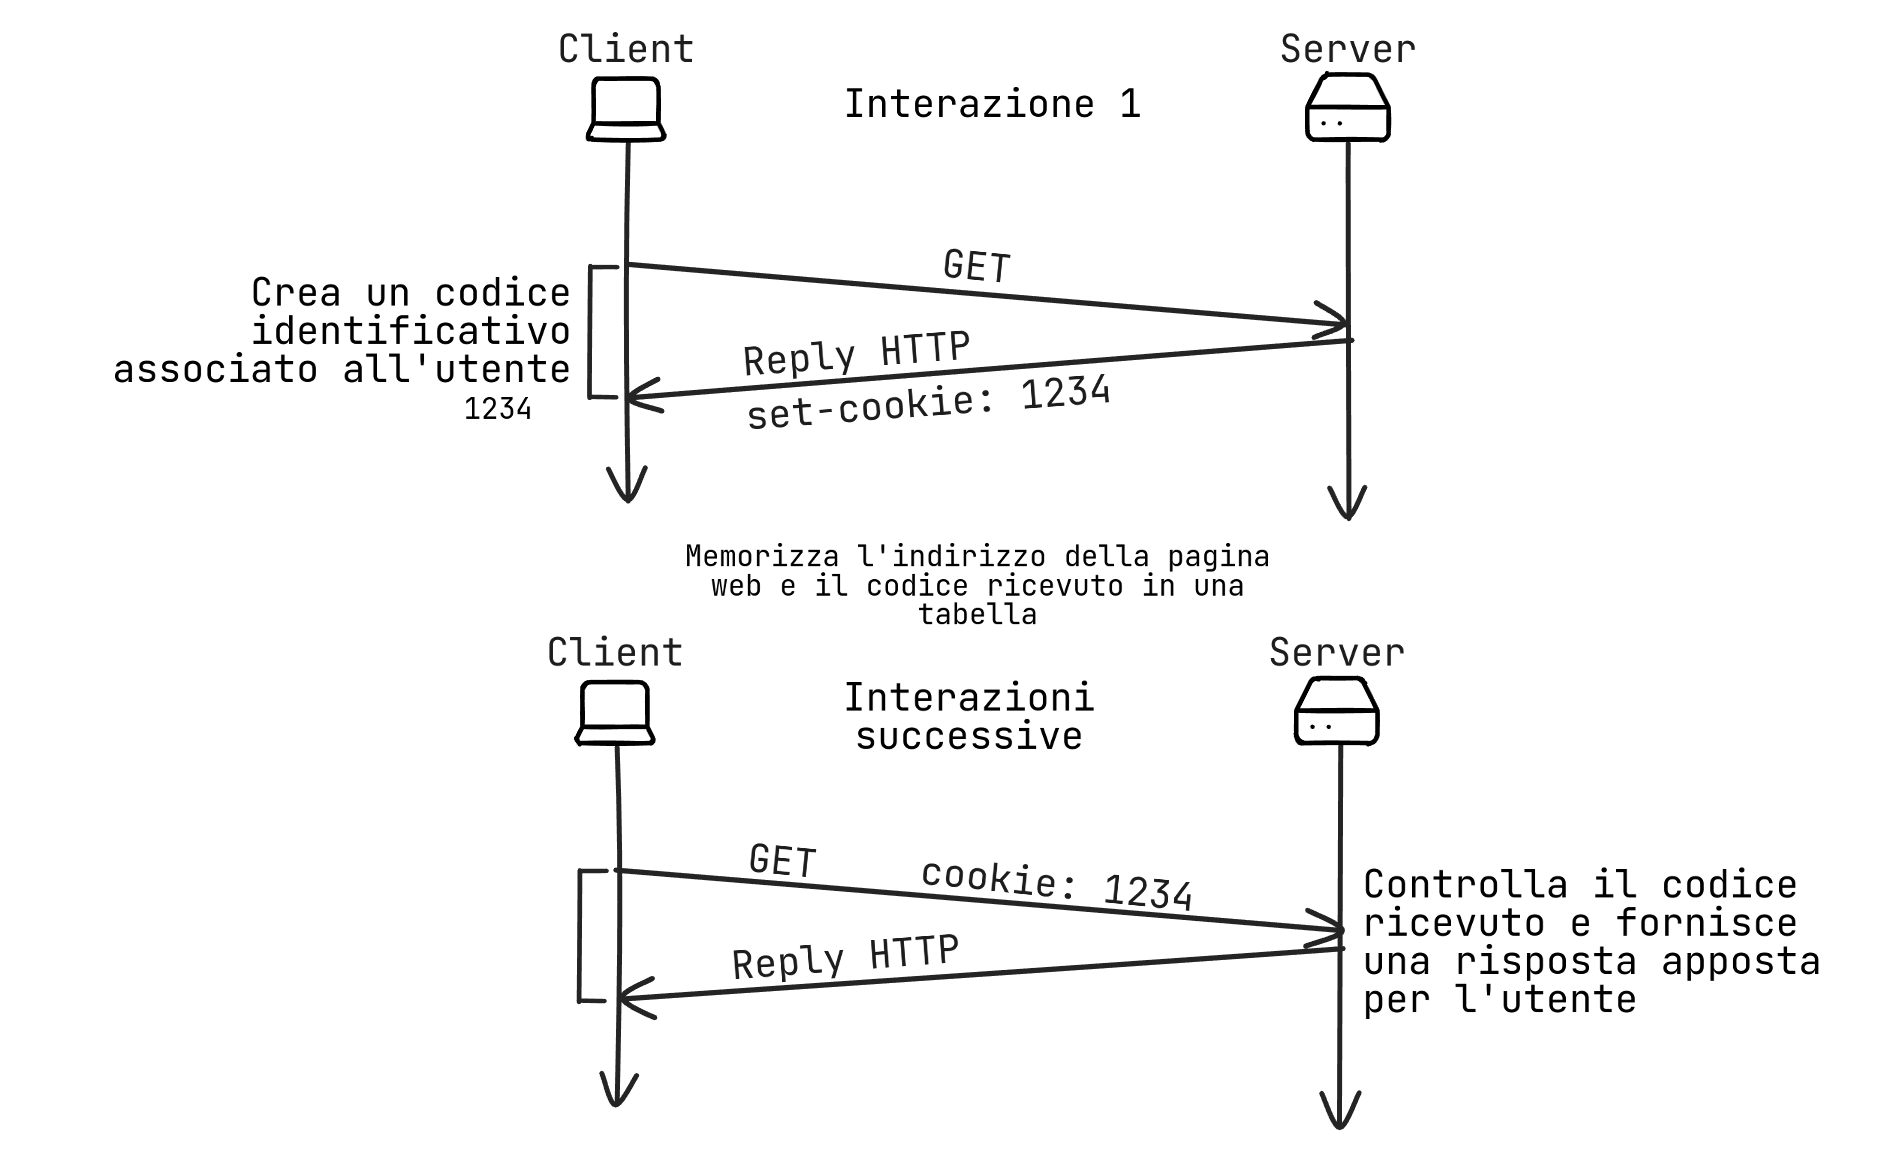
\includegraphics[width=1\textwidth]{cookies}
  \caption{Esempio di cookies}
\end{figure}

\vspace{1em}
\noindent
Per diminuire il ritardo di accesso alle risorse si usa un meccanismo di \textbf{caching}
che offre diversi vantaggi:
\begin{itemize}
  \item Si riduce il ritardo di accesso
  \item Viene diminuito il carico sui server
\end{itemize}
\begin{figure}[H]
  \centering
  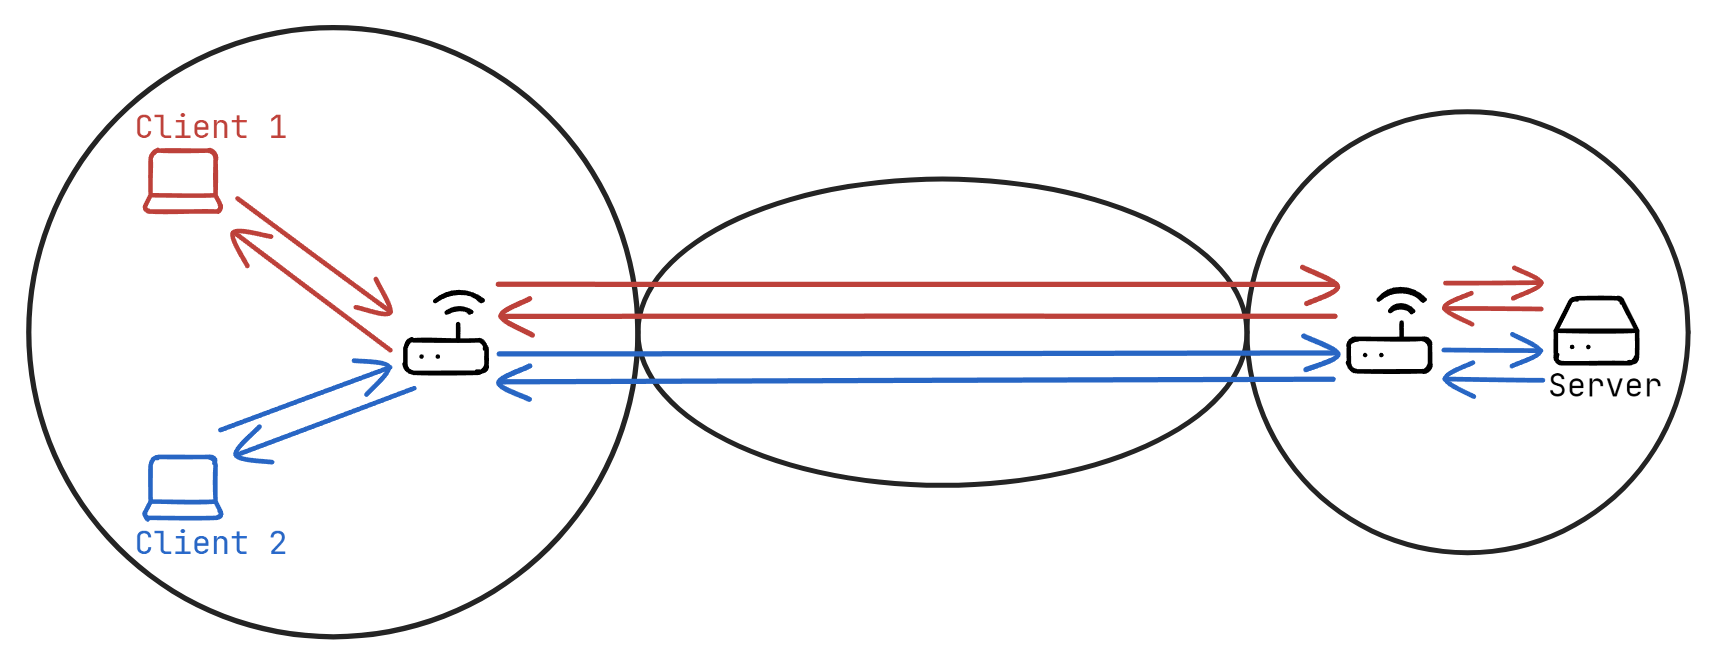
\includegraphics[width=0.9\textwidth]{traffico-client-server}
  \caption{Traffico senza cache}
\end{figure}
\noindent
Senza cache il ritardo che sente il secondo client è uguale al ritardo che sente il primo client e il
carico è doppio.
\begin{figure}[H]
  \centering
  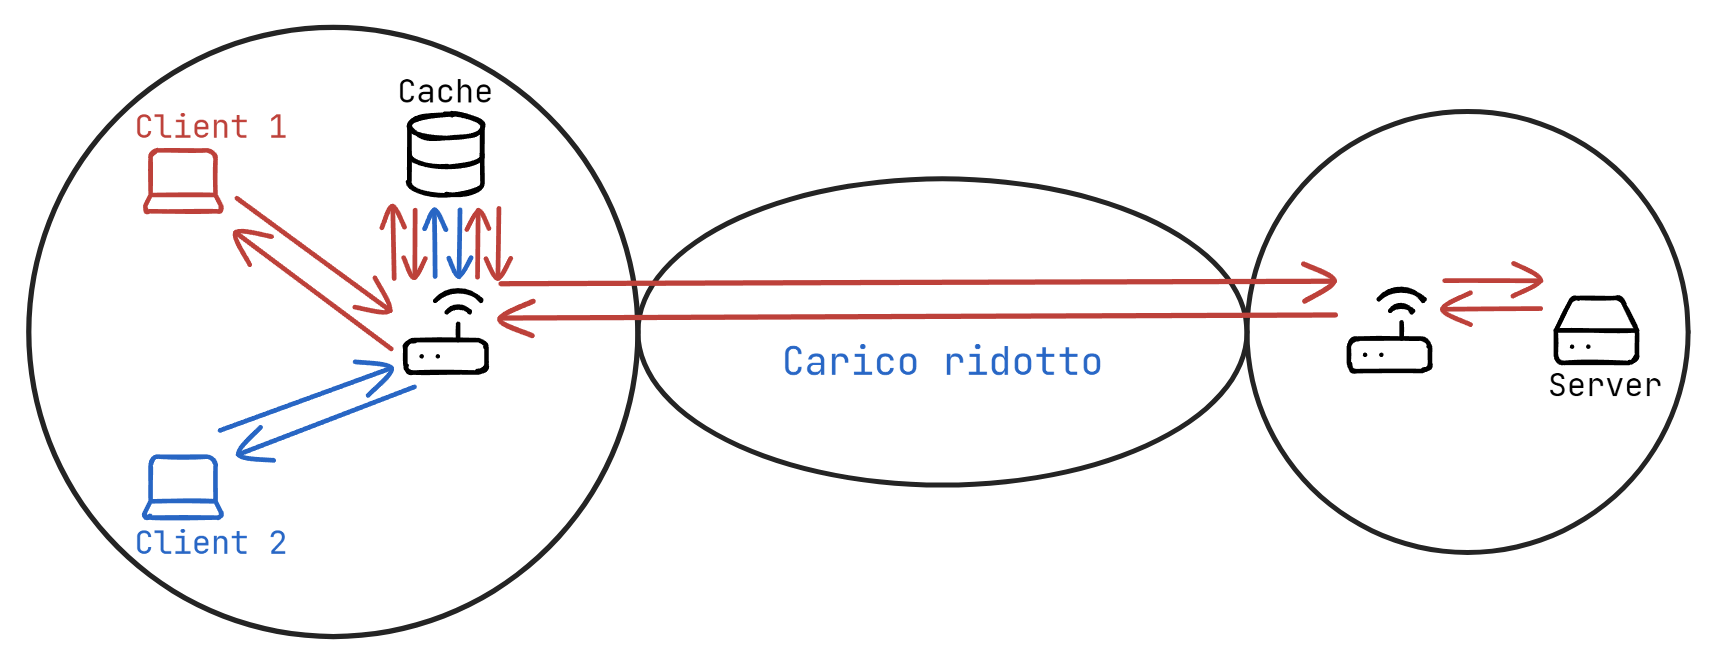
\includegraphics[width=0.9\textwidth]{traffico-client-server-cache}
  \caption{Traffico con la cache}
\end{figure}
\noindent
Con la cache il ritardo che sente il secondo client è minore e il carico è dimezzato 
perchè la cache contiene già i dati che il secondo client vuole siccome sono stati
caricati dal primo client.

\vspace{1em}
\noindent
Una buona cache lavora con un \( 70\%-80\% \) di \textbf{hit rate}. 

Se il contenuto sul server di origine cambia, la cache potrebbe contenere dati obsoleti.
Per risolvere questo problema, il protocollo HTTP prevede il metodo \textbf{GET condizionale}
in cui una riga di intestazione della richiesta è:
\begin{lstlisting}
  ...
  If-Modified-Since: <data>
\end{lstlisting}
\begin{figure}[H]
  \centering
  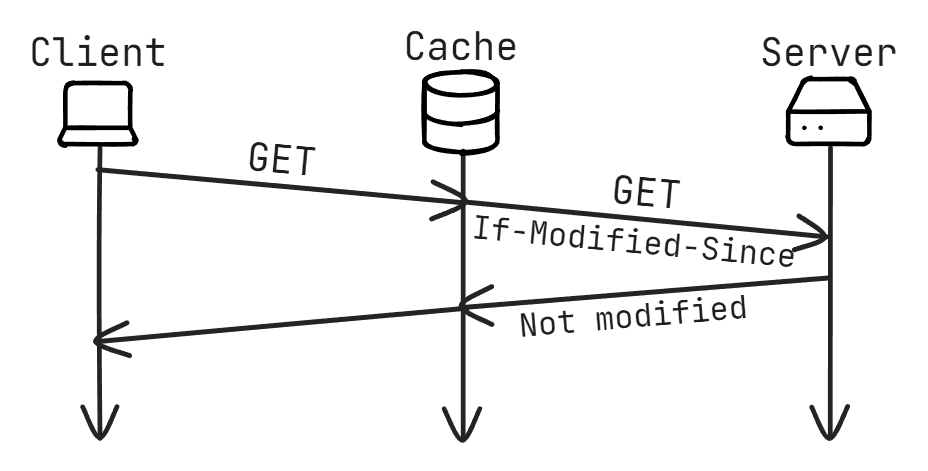
\includegraphics[width=0.75\textwidth]{comunicazione-cache}
  \caption{Comunicazione con la cache}
\end{figure}
\noindent
Nella risposta del server (la prima con il contenuto, o le successive con "not modified")
viene indicato anche il periodo di validità del contenuto:

\subsubsection{DNS (Domain name system)}
Lo scopo principale del DNS è la traduzione dei nomi logici (ad esempio\\
\texttt{www.univr.it}) nei corrispondenti indirizzi IP (ad esempio \texttt{157.27.0.1}).
Questo viene fatto tramite una tabella di traduzione che si trova in un server DNS.
\begin{figure}[H]
  \centering
  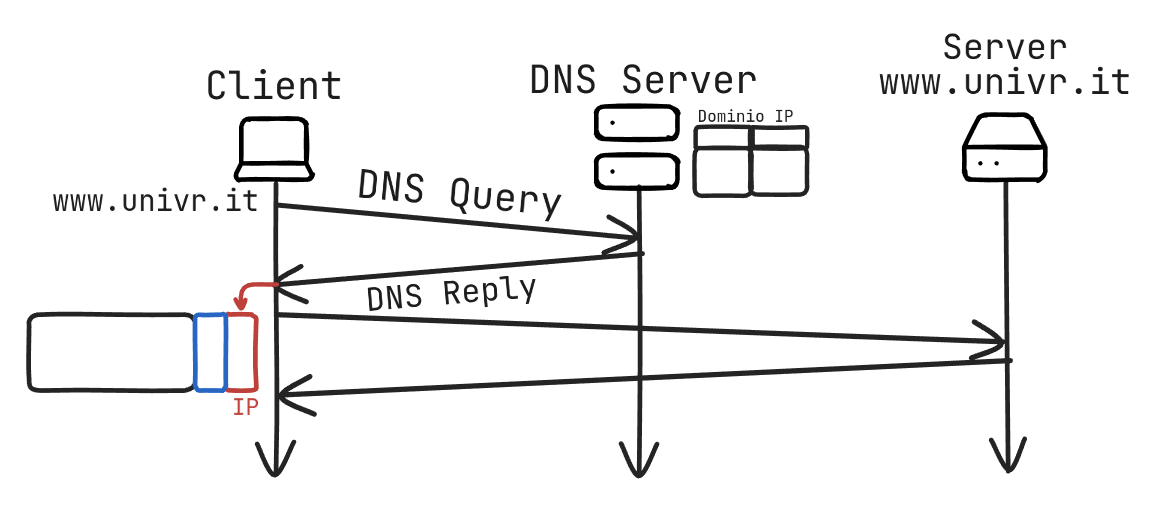
\includegraphics[width=0.75\textwidth]{comunicazione-dns}
  \caption{Comunicazione con il server DNS}
\end{figure}
Il server DNS ha un indirizzo IP statico:
\begin{itemize}
  \item Può essere inserito esplicitamente dall'utente dalle impostazioni di rete
  \item Viene fornito dalla rete stessa quando viene assegnato l'indirizzo IP (DHCP)
\end{itemize}
Per conoscere l'associazione tra i nomi logici e gli indirizzi IP, il server DNS
utilizza un database \textbf{distribuito} e \textbf{gerarchico}:
\begin{itemize}
  \item \textbf{Server DNS radice} (sono circa 7-10): Contengono i puntatori a una serie di server
    chiamati \textbf{server top level domain} (TLD)

  \item \textbf{Server Top Level Domain} (TLD): Gestiscono le informazioni relative
    ai domini di primo livello (ad esempio \texttt{.com}, \texttt{.it}, \texttt{.org}).
    Ciascun TLD punta a una serie di server chiamati \textbf{Server DNS Locali}.

  \item \textbf{Server DNS Locali}: Gestiscono il dominio di una organizzazione specifica
\end{itemize}
\begin{figure}[H]
  \centering
  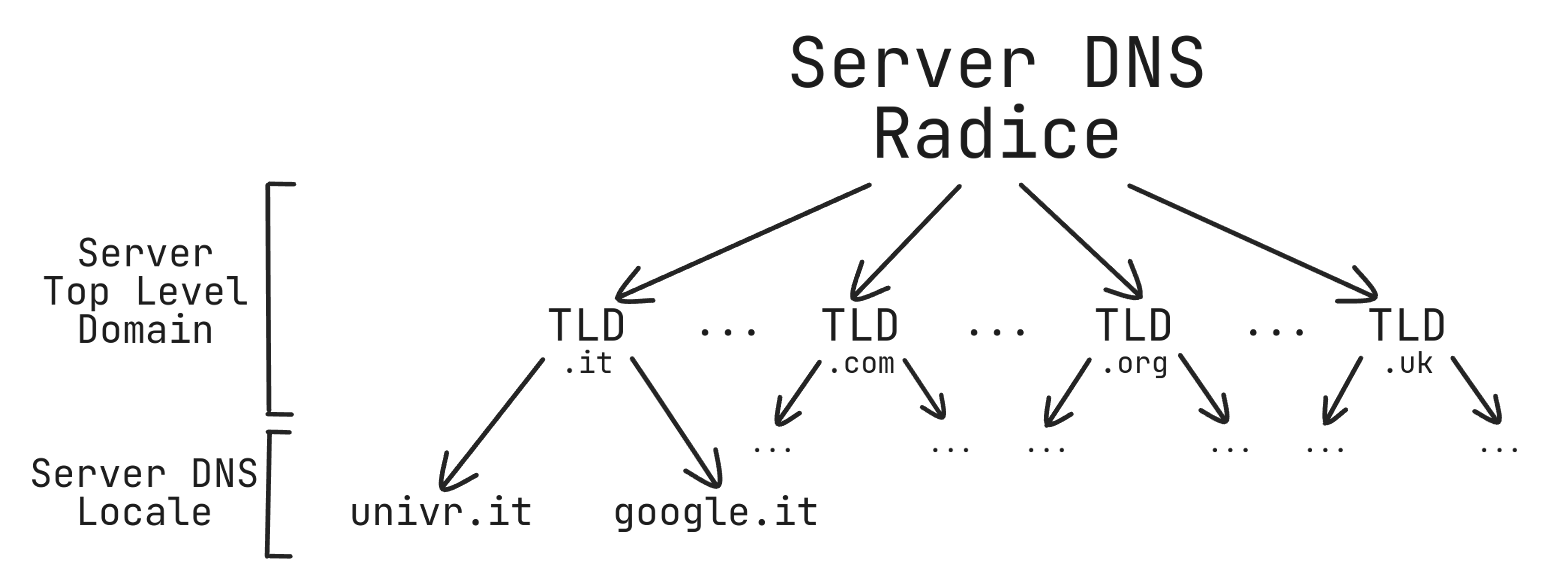
\includegraphics[width=0.85\textwidth]{albero-dns}
  \caption{Albero dei server DNS}
\end{figure}
Un indirizzo (URL) è composto da più parti separate da un punto:
\[
  \underbrace{\texttt{www}}_{\text{Server specifico}}.
  \underbrace{\texttt{univr}}_{\text{DNS Locali}}.
  \underbrace{\texttt{it}}_{\text{TLD}}
\]
Il client interagisce solamente con il server DNS locale:
\begin{figure}[H]
  \centering
  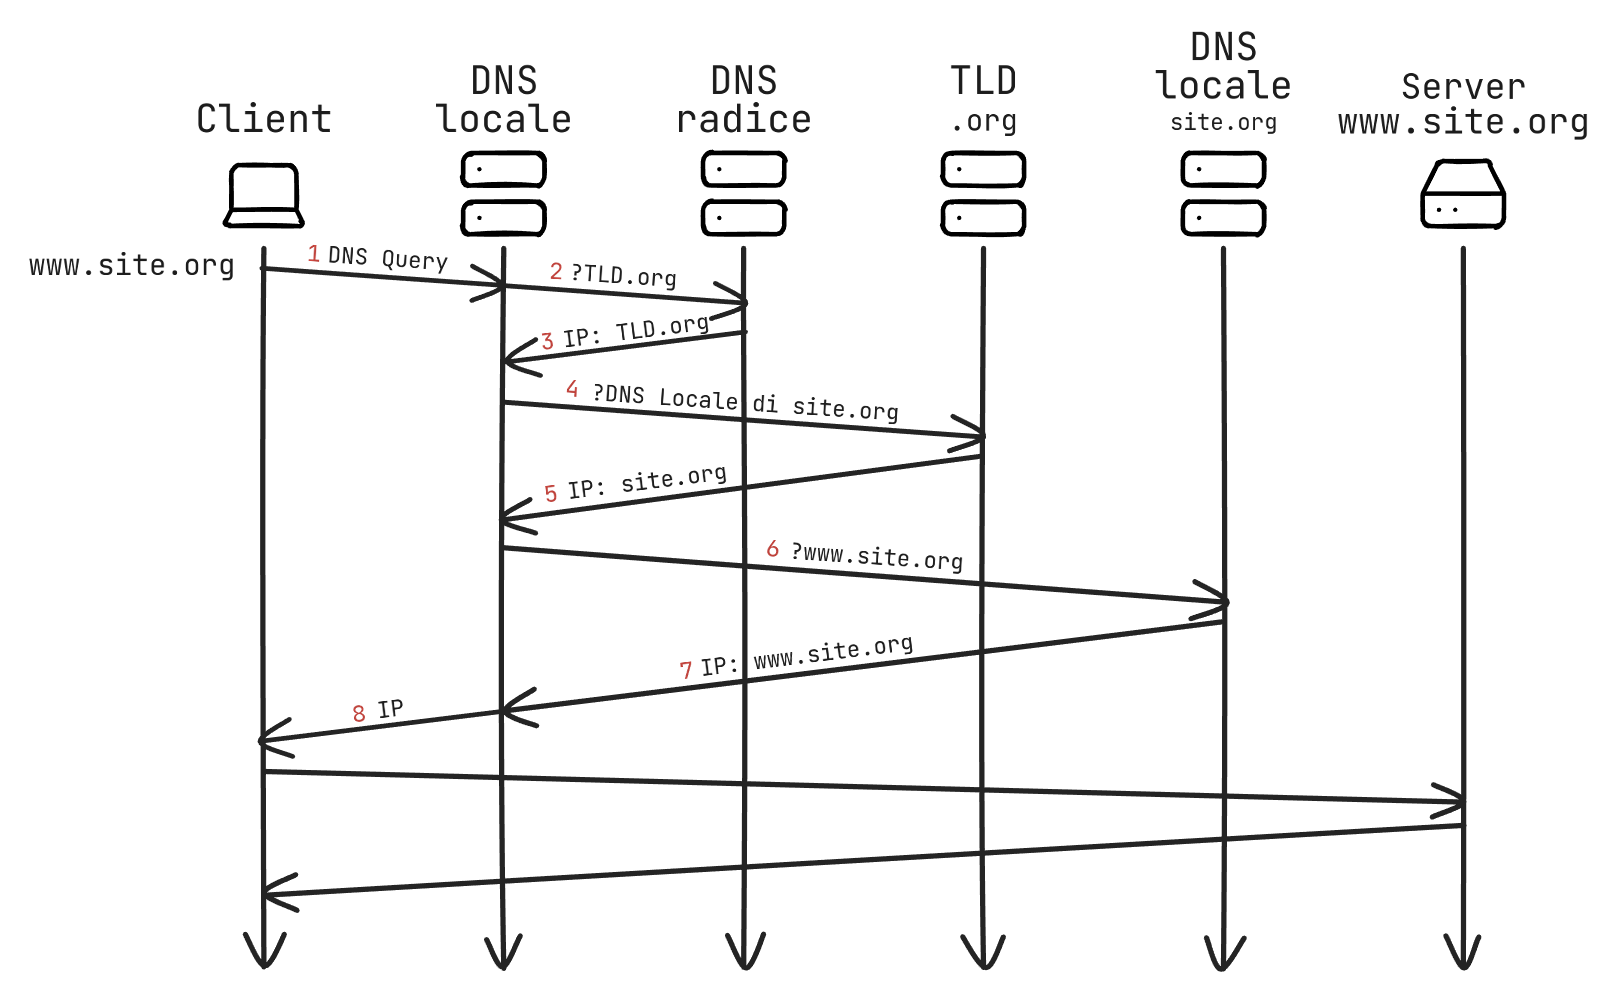
\includegraphics[width=1\textwidth]{client-dns-server}
  \caption{Comunicazione tra client e server tramite DNS}
\end{figure}
\begin{enumerate}
  \item Il client invia una richiesta al server DNS locale chiedendo l'indirizzo IP
    di un determinato nome logico
  \item Il server DNS locale manda una richiesta ad uno dei server radice salvati
    nella sua configurazione per ottenere l'indirizzo IP del server TLD
  \item Il server radice manda una risposta con l'indirizzo IP del server TLD
  \item Il server DNS locale manda una richiesta al server TLD per ottenere l'indirizzo
    IP del server DNS locale del sito richiesto
  \item Il server TLD manda una risposta con l'indirizzo IP del server DNS locale
  \item Il server DNS locale è in grado di contattare il server DNS locale del sito
    richiesto e chiede l'indirizzo IP del sito \texttt{www.site.org}
  \item Il server DNS locale manda una risposta con l'indirizzo IP del sito al DNS locale
  \item Una volta ricevuto l'IP, può essere inviato al client e venire utilizzato per
    contattare il server stesso
\end{enumerate}
Il server DNS locale memorizza le risposte, e quindi gli indirizzi IP dei server DNS TLD
e server DNS locali, con cui ha interagito recentemente.

\vspace{1em}
\noindent
Il rapporto tra il server DNS e la network cache è il seguente:
\begin{figure}[H]
  \centering
  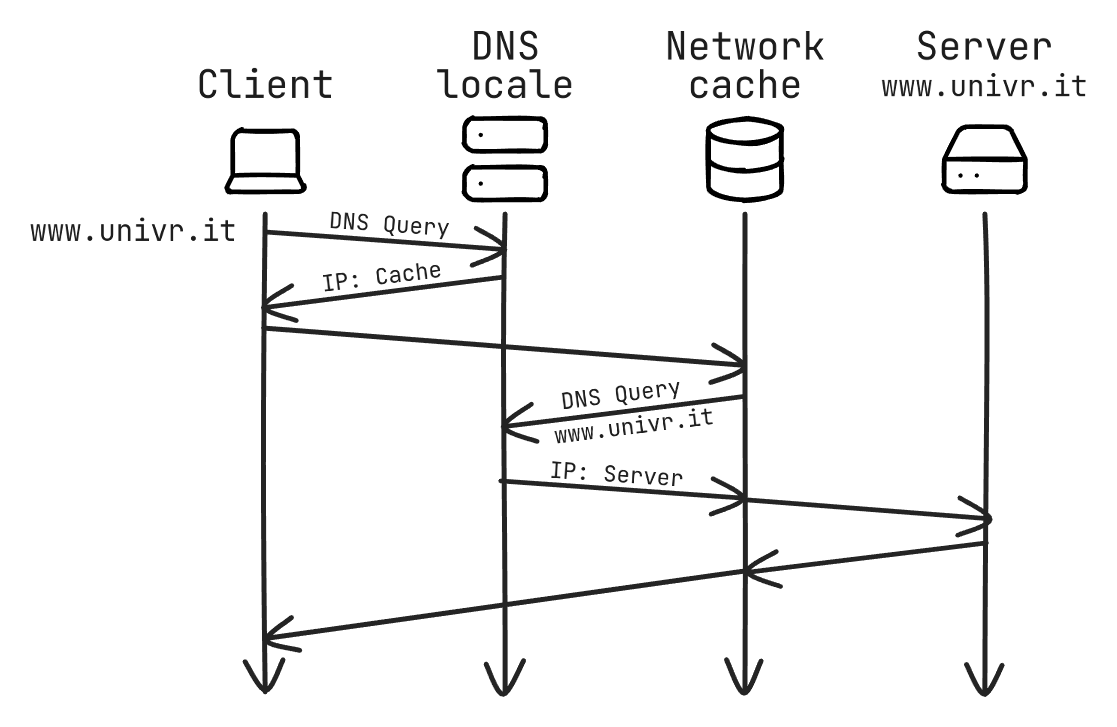
\includegraphics[width=0.75\textwidth]{dns-cache}
  \caption{Comunicazione tra client e server tramite DNS}
\end{figure}

\subsection{Protocolli di posta elettronica}
Ci sono diversi protocolli di posta elettronica che variano in base all'invio e alla 
ricezione:
\begin{itemize}
  \item \textbf{Invio}: SMTP (Simple Mail Transfer Protocol)
  \item \textbf{Ricezione}:
    \begin{itemize}
      \item POP (Post Office Protocol), non viene più utilizzato, perchè non sicuro
      \item IMAP (Internet Message Access Protocol)
      \item HTTP (Webmail)
    \end{itemize}
\end{itemize}
Tutti i protocolli si appoggiano su TCP. Dal punto di vista dell'architettura, ogni
dominio di posta elettronica (la porzione che segue la @) ha un server SMTP che gestisce 
caselle degli utenti appartenenti a quel dominio.
\begin{figure}[H]
  \centering
  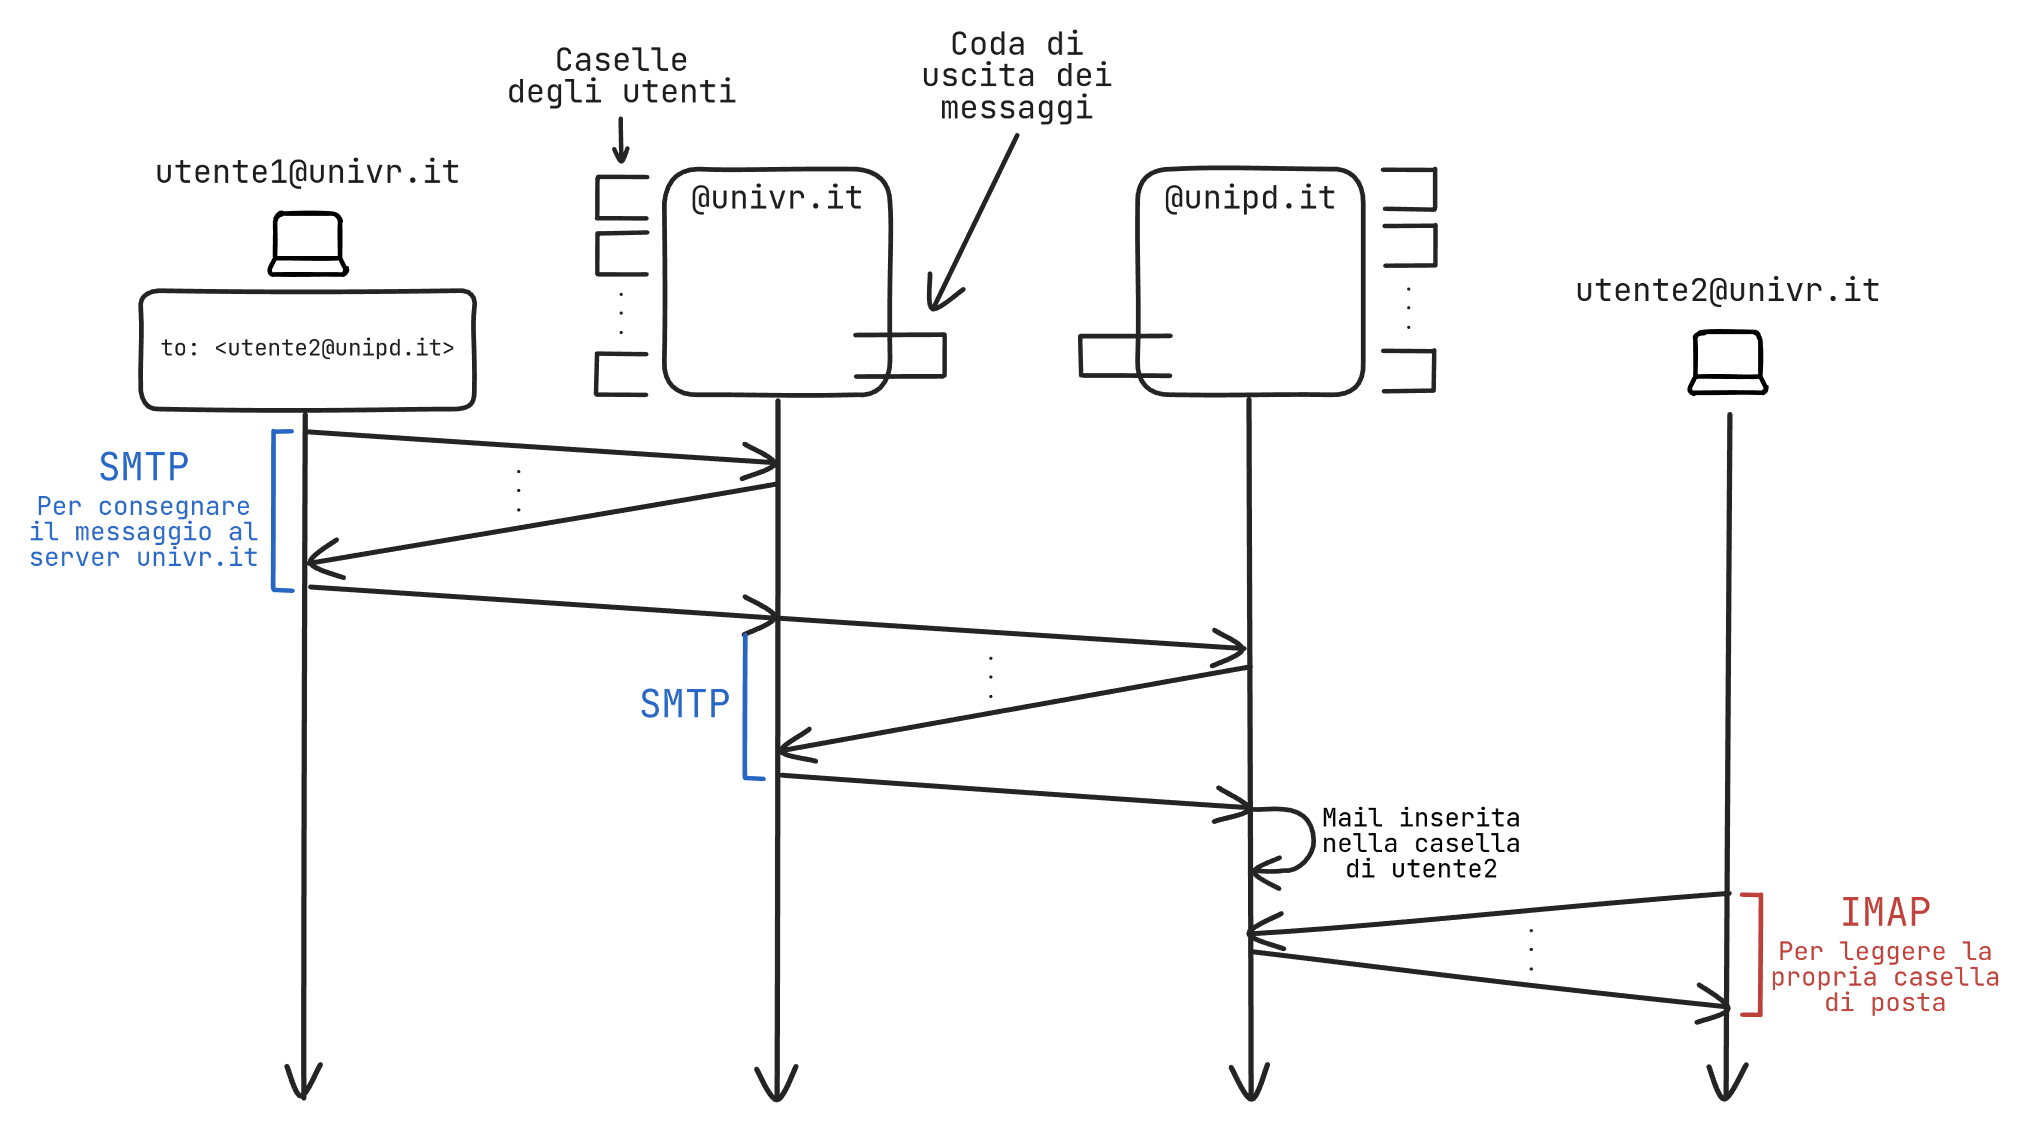
\includegraphics[width=1\textwidth]{smtp-imap}
  \caption{Invio e ricezione di posta elettronica}
\end{figure}
\noindent
Quando il server \texttt{univr.it} riceve un messaggio, controlla il dominio. Se il
dominio è \texttt{univr.it}, allora mette il messaggio nella casella di posta.
Se il dominio è diverso, il server SMTP contatta il server SMTP di destinazione per
la consegna del messaggio attraverso il protocollo SMTP.

\section{Livello di trasporto}
A livello di trasporto esistono 2 protocolli principali:
\begin{itemize}
  \item \textbf{TCP}
  \item \textbf{UDP}
\end{itemize}

\subsection{Protocollo TCP (Transmission Control Protocol)}
\subsubsection{Formato del pacchetto}
La grandezza dell'header TCP è di \( 20 byte \) tutti scritti in 5 righe da 4 byte. I
campi dell'header sono i seguenti:
\begin{figure}[H]
  \centering
  \begin{tikzpicture}
    \def\len{7}
    \def\hei{0.8}

    \draw (0,0) rectangle ++(\len/2,-\hei) node[midway] {Porta sorgente};
    \draw (\len/2,0) rectangle ++(\len/2,-\hei) node[midway] {Porta destinazione};

    \draw (0,-\hei) rectangle ++(\len,-\hei) node[midway] {Sequence number};
    \draw (0,-\hei*2) rectangle ++(\len,-\hei) node[midway] {Acknowledge number};

    \draw (0,-\hei*3) rectangle ++(\len/8,-\hei) node[midway,scale=0.9] {Offset};
    \draw (\len/8,-\hei*3) rectangle ++(\len*3/16,-\hei) node[midway,scale=0.9] {Reserved};
    \draw (\len/8+\len*3/16,-\hei*3) rectangle ++(\len*3/16,-\hei) node[midway,scale=0.9] {Flags};
    \draw (\len/2,-\hei*3) rectangle ++(\len/2,-\hei) node[midway] {Window};

    \draw (0,-\hei*4) rectangle ++(\len/2,-\hei) node[midway] {Checksum};
    \draw (\len/2,-\hei*4) rectangle ++(\len/2,-\hei) node[midway] {Urgent pointer};

    \draw[fill,fill opacity=0.1,text opacity=1] (0,-\hei*5) rectangle ++(\len,-\hei*2) node[midway] {Dati};

    \node[above,scale=0.7] at (0,0) {0};
    \node[above,scale=0.7] at (\len/2,0) {15};
    \node[above,scale=0.7] at (\len,0) {31};
  \end{tikzpicture}
  \caption{Formato del pacchetto TCP}
\end{figure}
\begin{itemize}
  \item \textbf{Porta sorgente/destinazione} (bit 0-16): Identificatori dei processi 
    sorgente e destinazione coinvolti nella comunicazione. Ci sono 2 tipi di porte:
    \begin{itemize}
      \item \textbf{Porte statiche}: Vanno dalla 0 alla 1023 e sono identificativi
        associati a protocolli definiti dallo standard (HTTP,SMTP,...) utilizzati
        \textbf{lato server}, quindi un client non può utilizzarle.

      \item \textbf{Porte dinamiche}: Vanno dalla 1024 alla 65535 e sono identificativi
        assegnati dal sistema operativo lato client quando viene aperto un socket.
    \end{itemize}

  \item \textbf{Sequence number}: 
    \begin{itemize}
      \item A livello applicativo vengono generati messaggi di
        dimensione arbitraria.
      \item A livello "collegamento dati" alla scheda di rete è associato un parametro
        chiamato \textbf{MTU} (Maximum Transmission Unit) che indica la dimensione
        massima di un pacchetto che può essere inviato. Il MSS (Maximum Segment Size)
        indica la dimensione massima di un segmento che può essere inviato.
    \end{itemize}
    Il sequence number identifica l'ordine dei segmenti rispetto al messaggio originale.
    Viene anche chiamato \textbf{offset rispetto al byte iniziale del segmento} e ad
    ogni sequence number viene sommata una costante uguale per ogni segmento chiamata
    \textbf{Initial Sequence Number} (ISN).
    \begin{figure}[H]
      \centering
      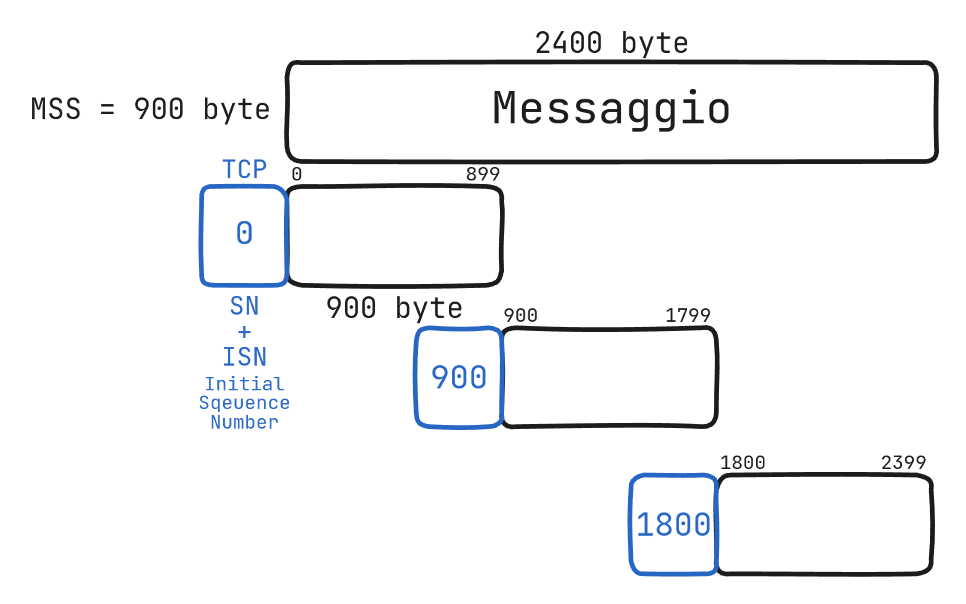
\includegraphics[width=0.7\textwidth]{segmentazione}
      \caption{Segmentazione di un messaggio}
    \end{figure}

  \item \textbf{Acknowledgment number}: Il TCP è un protocollo affidabile, cioè garantisce
    la consegna di tutti i segmenti, quindi c'è bisogno di un meccanismo di conferma
    della ricezione. Questo meccanismo è chiamato \textbf{Positive acknowledgment with
    retransmission} e quindi per ogni segmento ricevuto il destinatario manda un
    acknowledgment con il sequence number del prossimo segmento che si aspetta, ad
    esempio:
    \begin{example}
      Prendendo come esempio la segmentazione del messaggio precedente si ha:
      \begin{figure}[H]
        \centering
        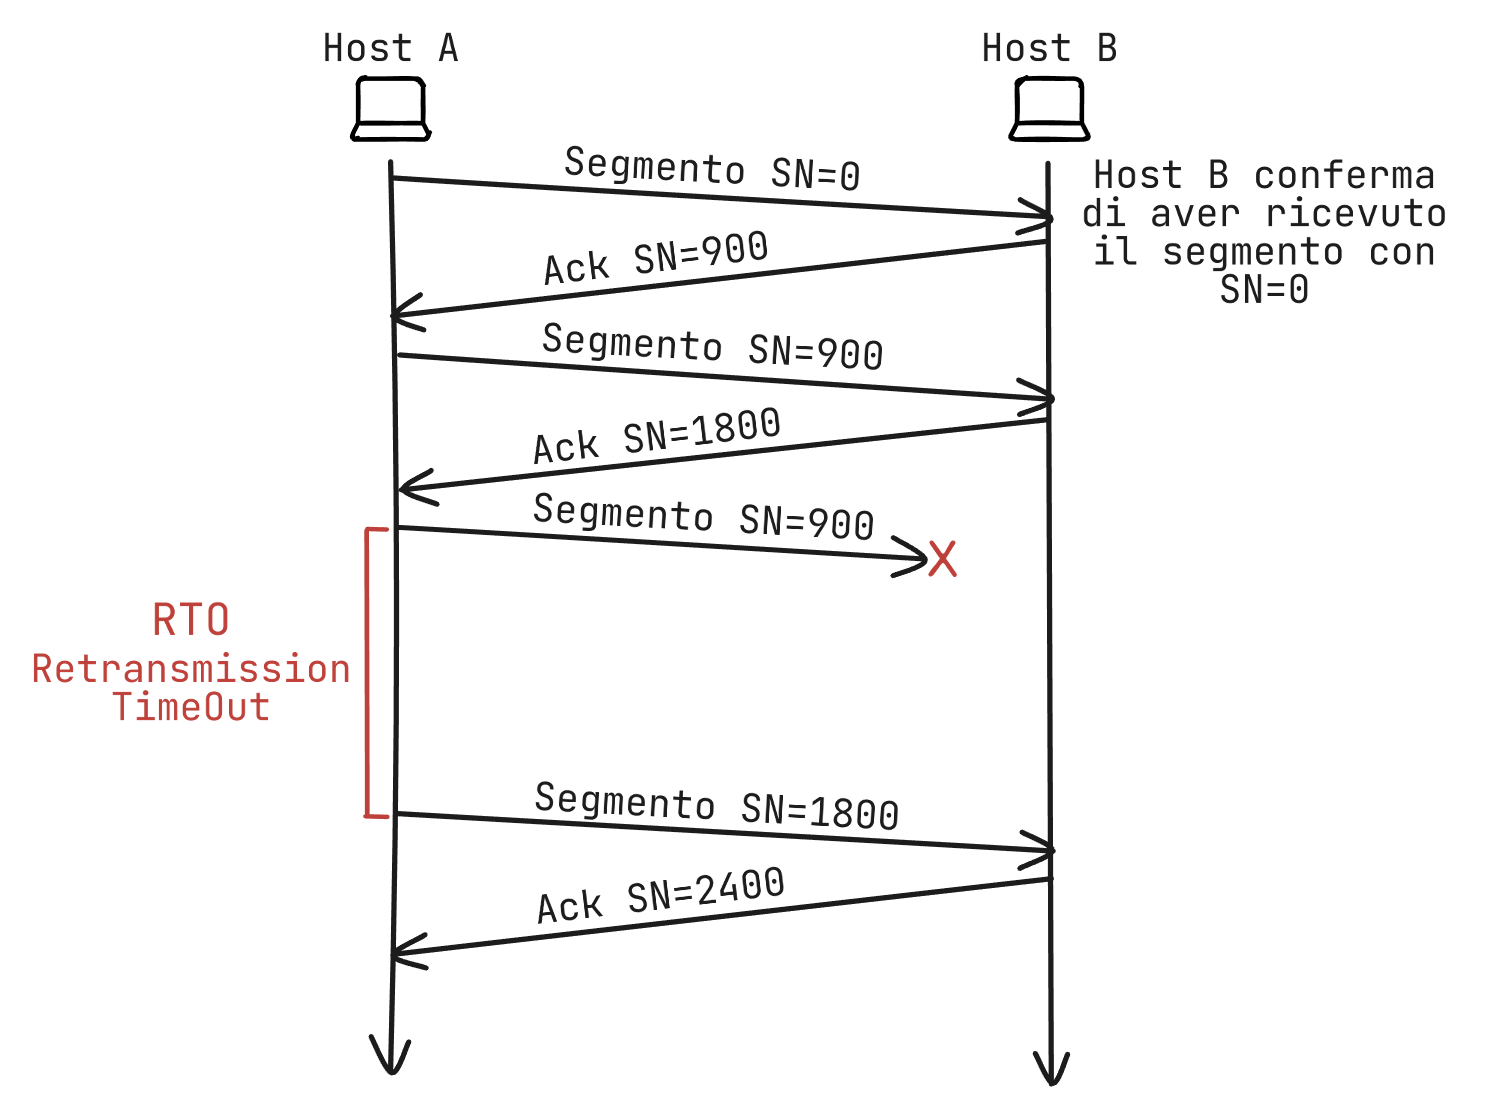
\includegraphics[width=1\textwidth]{rto}
        \caption{Positive acknowledgment with retransmission}
      \end{figure}
    \end{example}

    \vspace{1em}
    \noindent
    Un acknowledgment è un segmento TCP senza dati, quindi ha solamente l'header.

  \item \textbf{Offset}: Questo campo serve per indicare la grandezza dell'header e
    serve a sapere se ci sono delle opzioni aggiuntive.

  \item \textbf{Reserved}: Questo campo è riservato per usi futuri o per le opzioni.

  \item \textbf{Checksum}: Serve per controllare la presenza di errori nel segmento.
    La checksum è il risultato di una funzione che prende in input il segmento e restituisce
    un valore a dimensione fissa univoco per quel segmento. Se il segmento viene modificato
    durante la trasmissione, la checksum cambia e il destinatario fa un controllo
    mettendo in input ciò che ha ricevuto e se il confronto:
    \begin{itemize}
      \item Va a buon fine: con \textbf{alta probabilità} non ci sono stati errori
      \item Non va a buon fine: ci sono \textbf{sicuramente} errori e il segmento
        viene scartato
    \end{itemize}
    \begin{figure}[H]
      \centering
      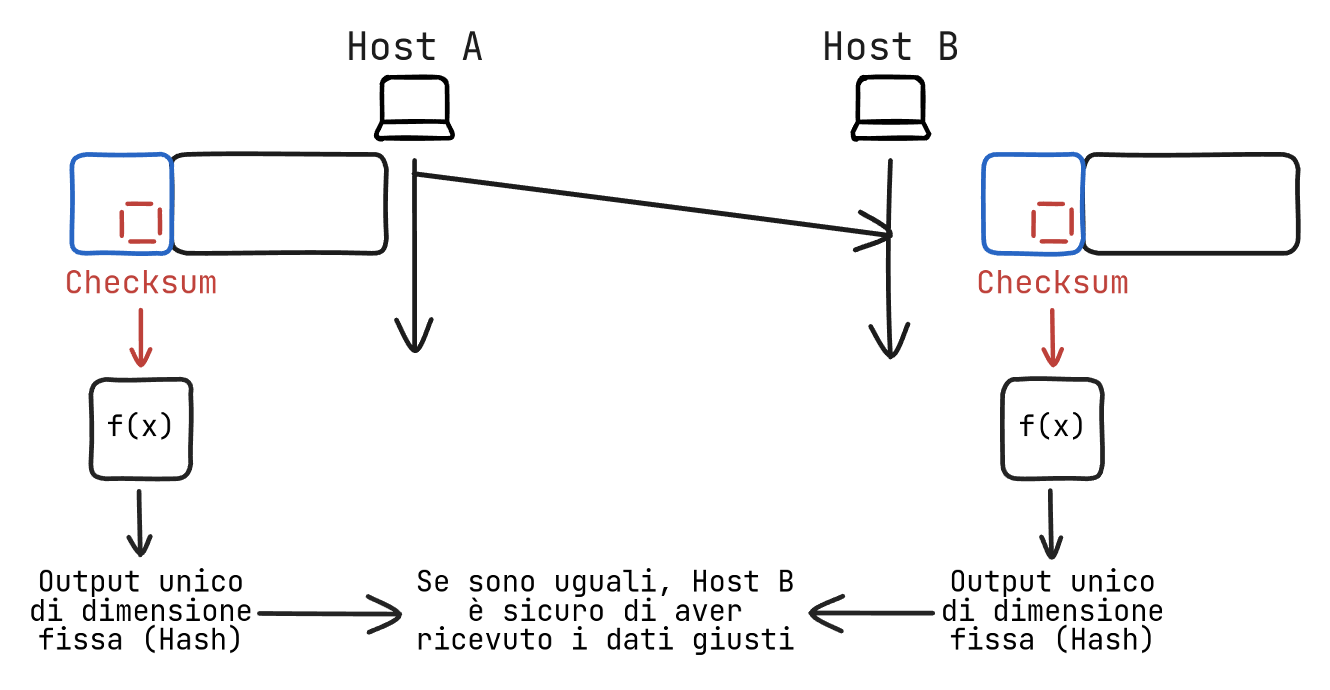
\includegraphics[width=0.8\textwidth]{checksum}
      \caption{Checksum}
    \end{figure}
\end{itemize}

\subsubsection{Gestione delle connessioni}
TCP è un protocollo \textbf{connection oriented}, cioè prima di scambiare dati, client
e server devono stabilire che vogliono comunicare e questo avviene tramite l'invio di
messaggi di servizio (senza dati), questa fase è chiamata \textbf{instaurazione della 
connessione}.

\vspace{1em}
\noindent
\textbf{N.B.}:
Instaurare una connessione non ha niente a che fare con la creazione di un circuito
o riservare delle risorse di rete

\vspace{1em}
\noindent
Quindi avviene uno scambio di segmenti TCM (header senza payload) chiamata
\textbf{Three-way handshake}:
\begin{figure}[H]
  \centering
  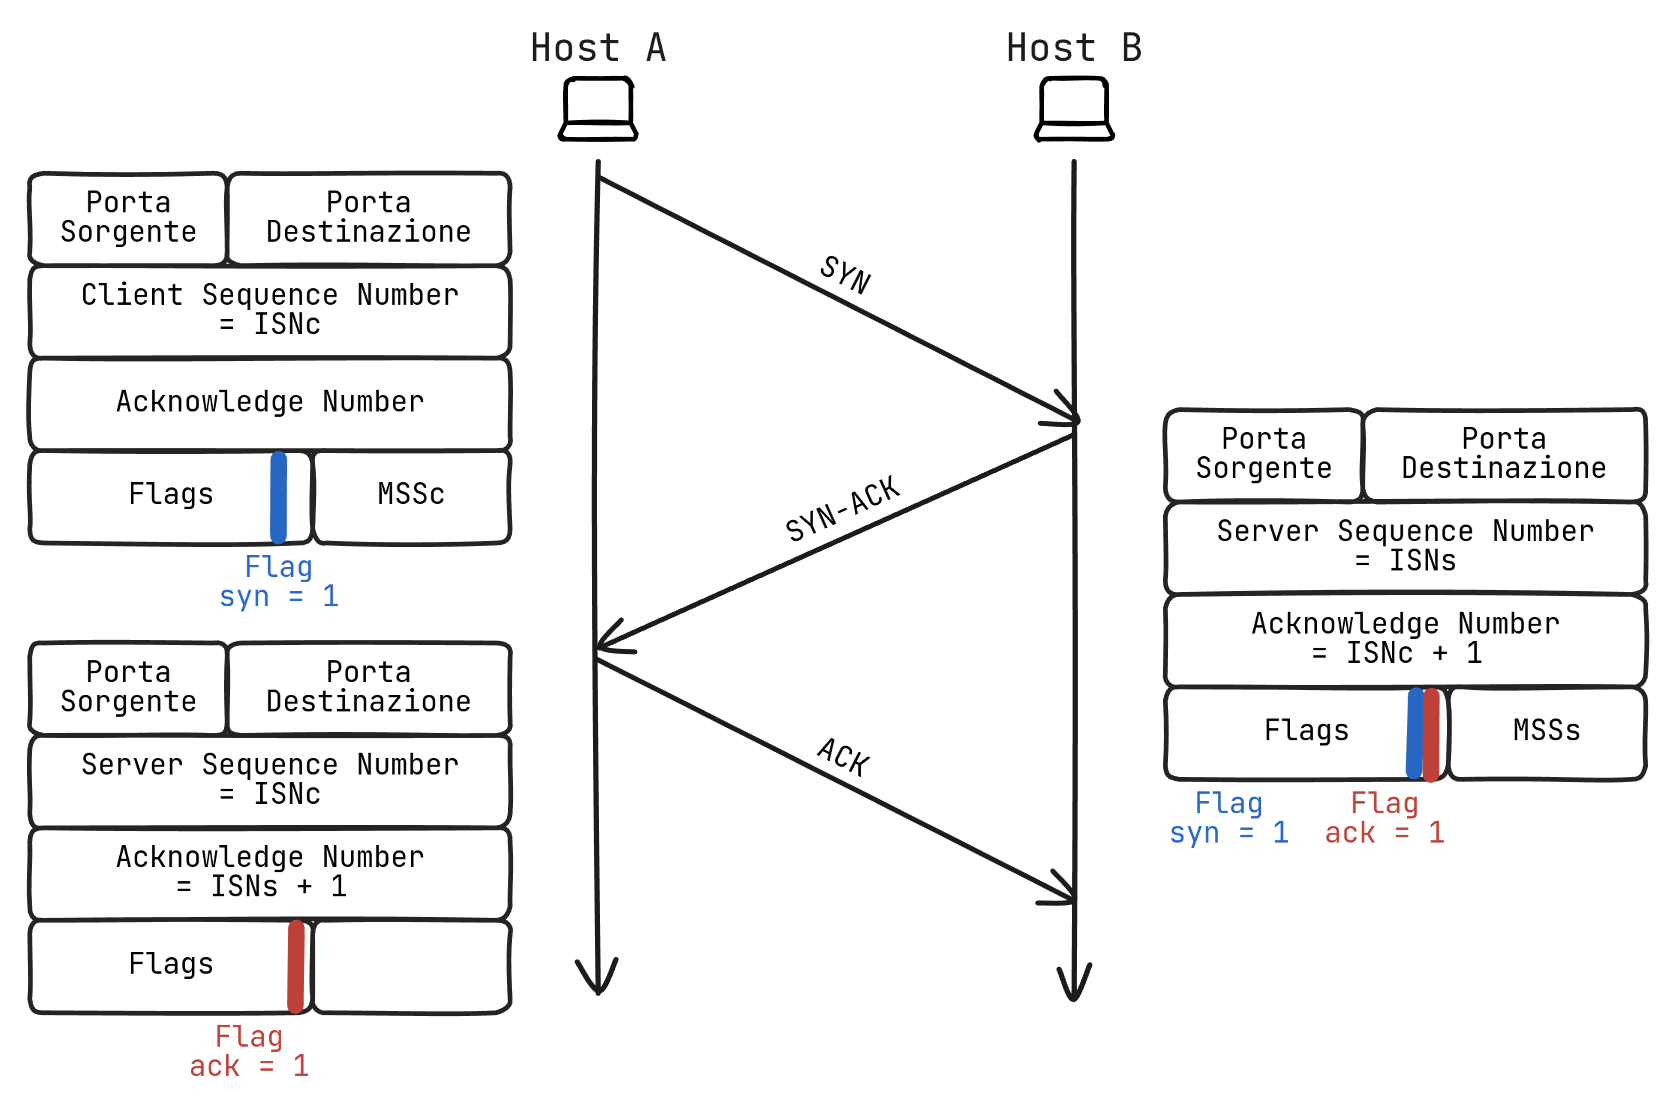
\includegraphics[width=1\textwidth]{three-way-handshake}
  \caption{Three-way handshake}
\end{figure}
\begin{itemize}
  \item \textbf{Syn}: Il client invia un segmento con il flag \texttt{SYN} a 1.
    Questo segmento contiene l'initial sequence number del client (ISN), cioè un numero 
    scelto casualmente da cui il client inizia a numerare i byte inviati. Questo numero
    serve anche come ulteriore sicurezza per la cifratura.

  \item \textbf{Syn-Ack}: Il server risponde con un segmento con i flag \texttt{SYN} e
    \texttt{ACK} a 1. Questo segmento contiene l'initial sequence number del server e
    l'acknowledgment number uguale all'ISN del client + 1.

  \item \textbf{Ack}: Il client risponde con un segmento con il flag \texttt{ACK} a 1 e
    l'acknowledgment number uguale all'ISN del server + 1.

  \item \textbf{Altri parametri}:
    \begin{itemize}
      \item \textbf{MSS} (Maximum Segment Size): Indica la dimensione massima di un
        segmento che il client e il server possono ricevere. Client e server utilizzeranno
        il valore minimo tra le 2 MSS comunicate. La MSS è contenuta nelle opzioni
        dell'header TCP, che sono utilizzate solo se necessario.
    \end{itemize}
\end{itemize}
Dopo aver instaurato la connessione gli host si possono scambiare i messaggi:
\begin{figure}[H]
  \centering
  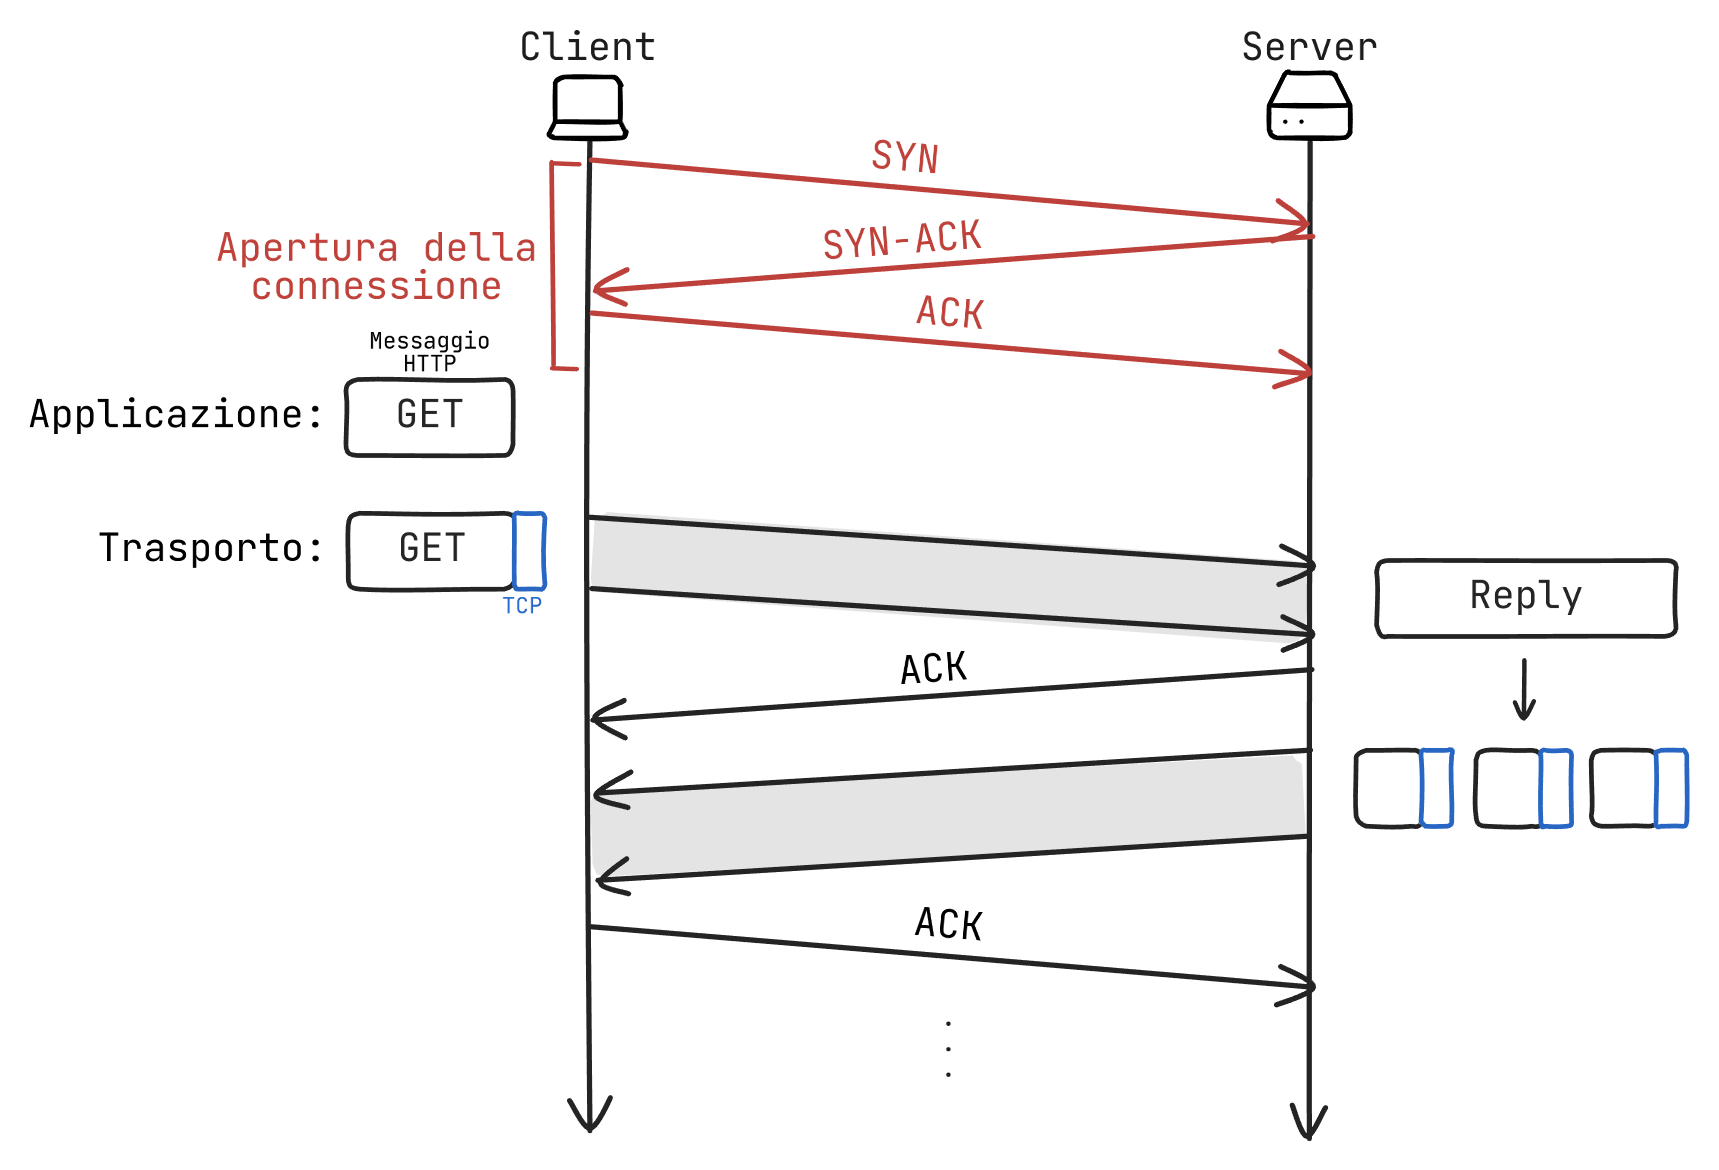
\includegraphics[width=1\textwidth]{connessione}
  \caption{Connessione TCP}
\end{figure}
\noindent
Quando lo scambio dei messaggi è terminato, la connessione viene chiusa attraverso uno
scambio di header. Siccome il canale è biirezionale, la chiusura deve avvenire
indipendentemente nelle due direzioni. I 2 messaggi sono:
\begin{itemize}
  \item \textbf{FIN}: Sarà un messaggio con il flag \texttt{FIN} a 1
  \item \textbf{ACK}: Sarà un messaggio con il flag \texttt{ACK} a 1
\end{itemize}
\begin{figure}[H]
  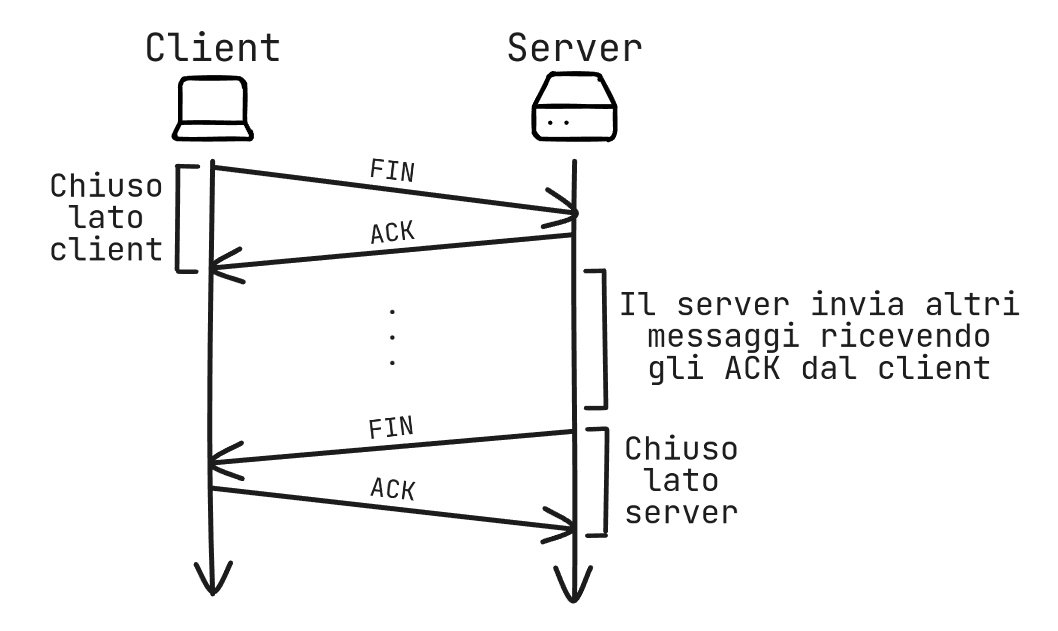
\includegraphics[width=0.45\textwidth]{fin1}
  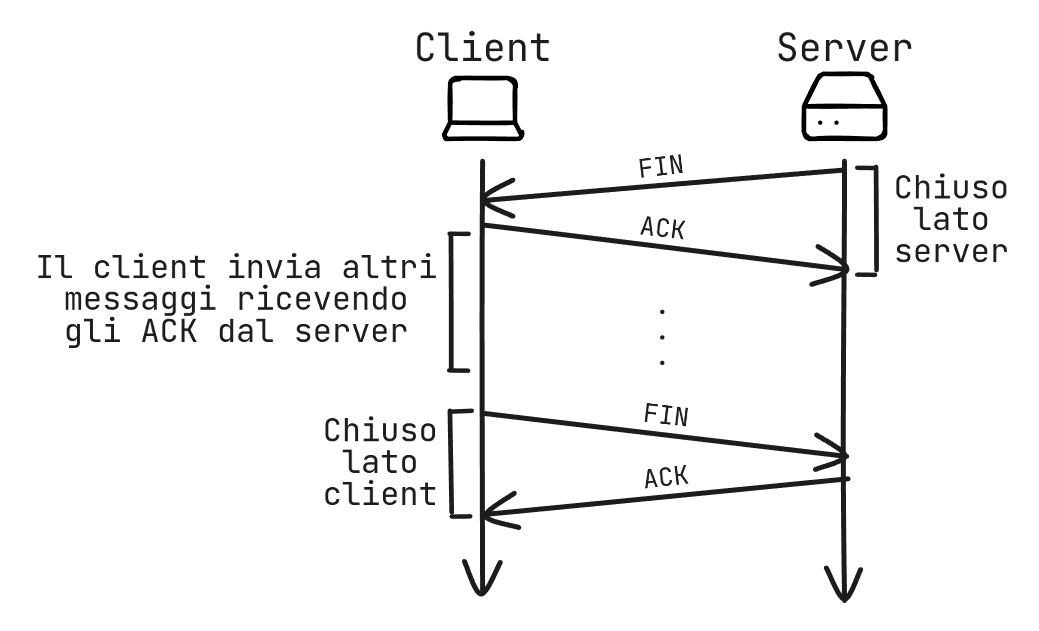
\includegraphics[width=0.45\textwidth]{fin2}
  \caption{Chiusura non simultanea}
\end{figure}
\begin{figure}[H]
  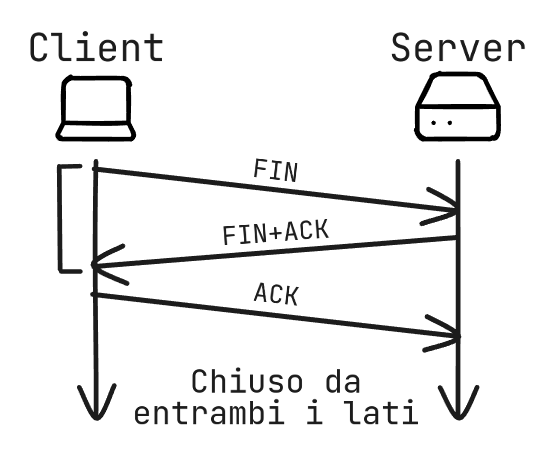
\includegraphics[width=0.45\textwidth]{fin3}
  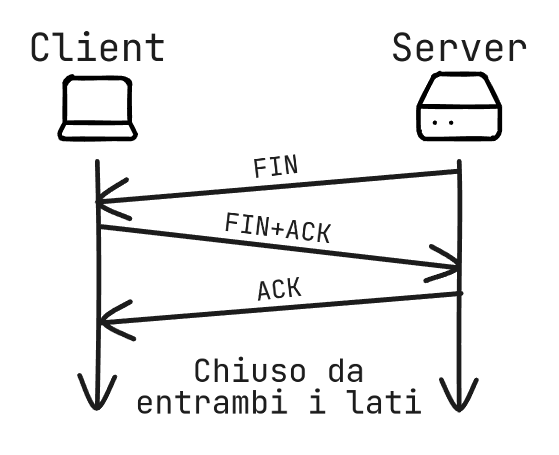
\includegraphics[width=0.45\textwidth]{fin4}
  \caption{Chiusura simultanea}
\end{figure}

\subsubsection{Affidabilità}
TCP è un protocollo \textbf{affidabile}, cioè quando un host invia un segmento si aspetta
di ricevere il riscontro entro un tempo massimo (RTO, Retransmission TimeOut).
\begin{figure}[H]
  \centering
  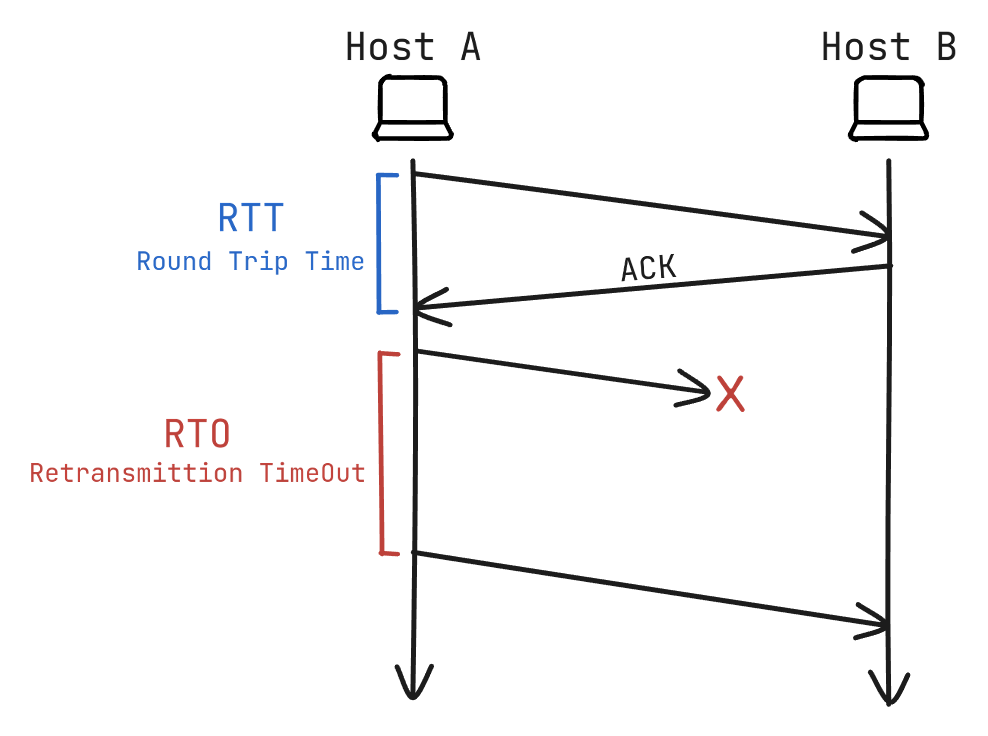
\includegraphics[width=0.8\textwidth]{rto2}
  \caption{Affidabilità}
\end{figure}
\noindent
L'RTO dovrà tenere in conto l'RTT (Round Trip Time), cioè il tempo che intercorre tra
l'invio di un segmento e la ricezione del corrispondente \texttt{ACK}.
All'apertura della connessione si misura il RTT durante il Three-way handshake.
\begin{figure}[H]
  \centering
  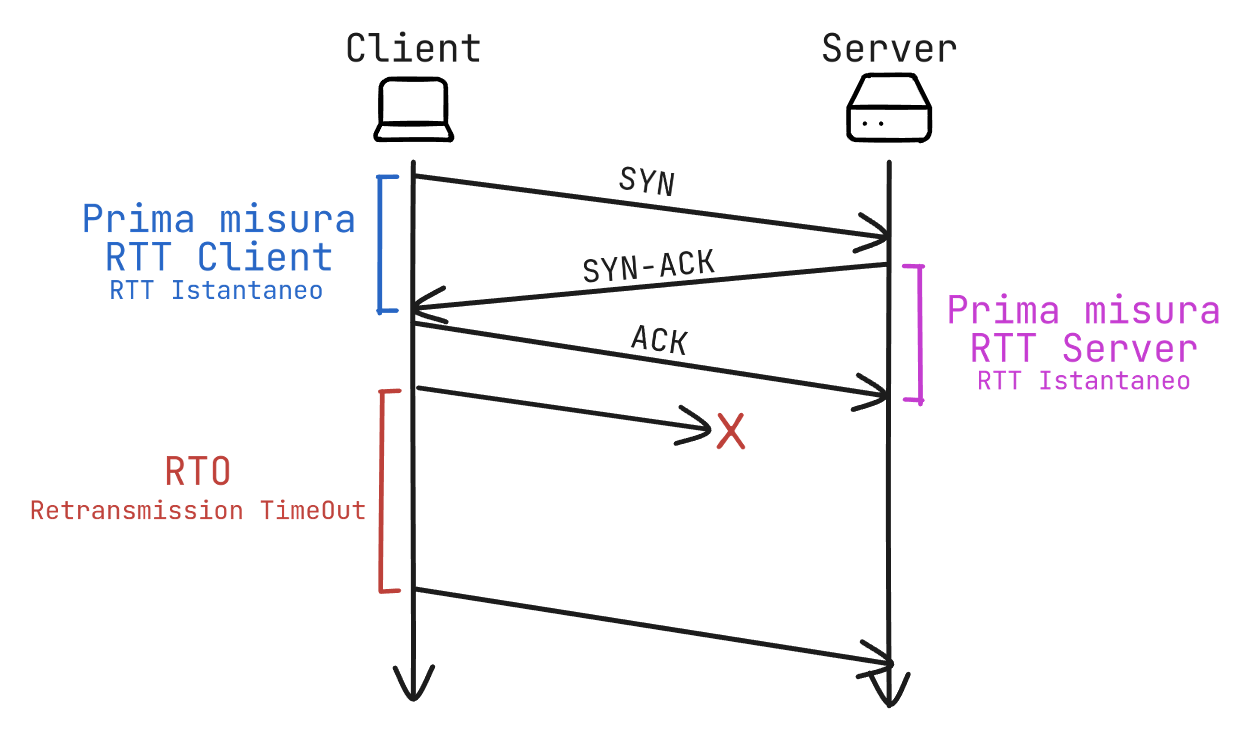
\includegraphics[width=0.8\textwidth]{rtt-istantaneo}
  \caption{RTT istantaneo}
\end{figure}

\noindent
Per l'invio del primo messaggio \texttt{SYN} il RTO è impostato a \( 500ms \) (caso
peggiore).
Per aggiornare i valori di RTT e RTO ogni host, per ogni segmento inviato, misura 
l'RTT istantaneo e usa tale valore per aggiornare una variabile chiamata \texttt{SRTT}
(Smoothed Round Trip Time).
\[
  SRTT_{\text{attuale}} = \alpha \cdot SRTT_{\text{precedente}} + (1 - \alpha) \cdot
  RTT_{\text{istantaneo}}
\] 
dove \( 0 < \alpha < 1\) che di solito vale \( \frac{7}{8} \).
\begin{figure}[H]
  \centering
  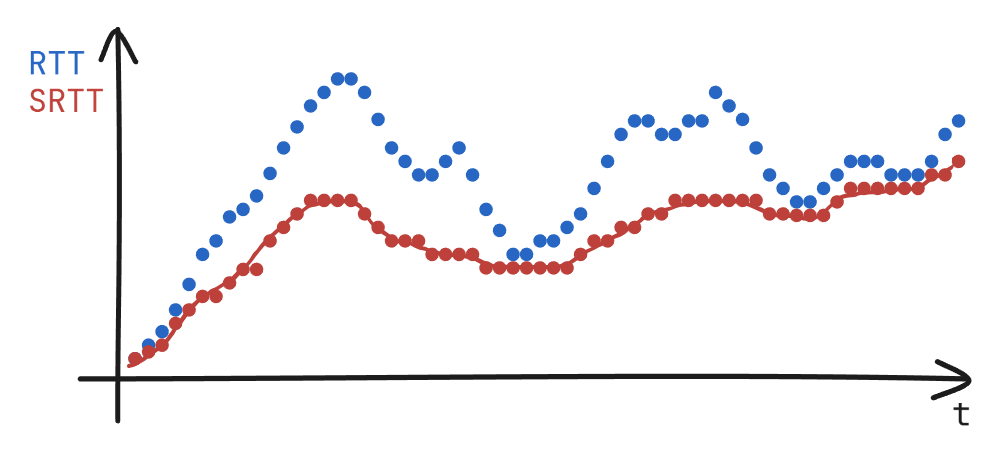
\includegraphics[width=0.8\textwidth]{srtt}
  \caption{SRTT}
\end{figure}
\noindent
Quindi l'SRTT è una \textbf{stima del valore medio} del RTT calcolata tramite 
l'Exponential Weighted Moving Average (EWMA). Questo metodo di calcolo è efficiente
perchè non deve tenere in memoria tutta la sequenza, ma solo l'ultimo valore.

\vspace{1em}
\noindent
Dato l'SRTT, l'RTO è pari a:
\[
  RTO = \beta \cdot SRTT_{\text{attuale}}
\] 
dove solitamente \( \beta = 2 \). L'RTO si \textbf{adatta dinamicamente} alla variazione
del RTT. In caso di perdite, il RTO per il segmento ritrasmesso viene temporaneamente
raddoppiato.
\begin{figure}[H]
  \centering
  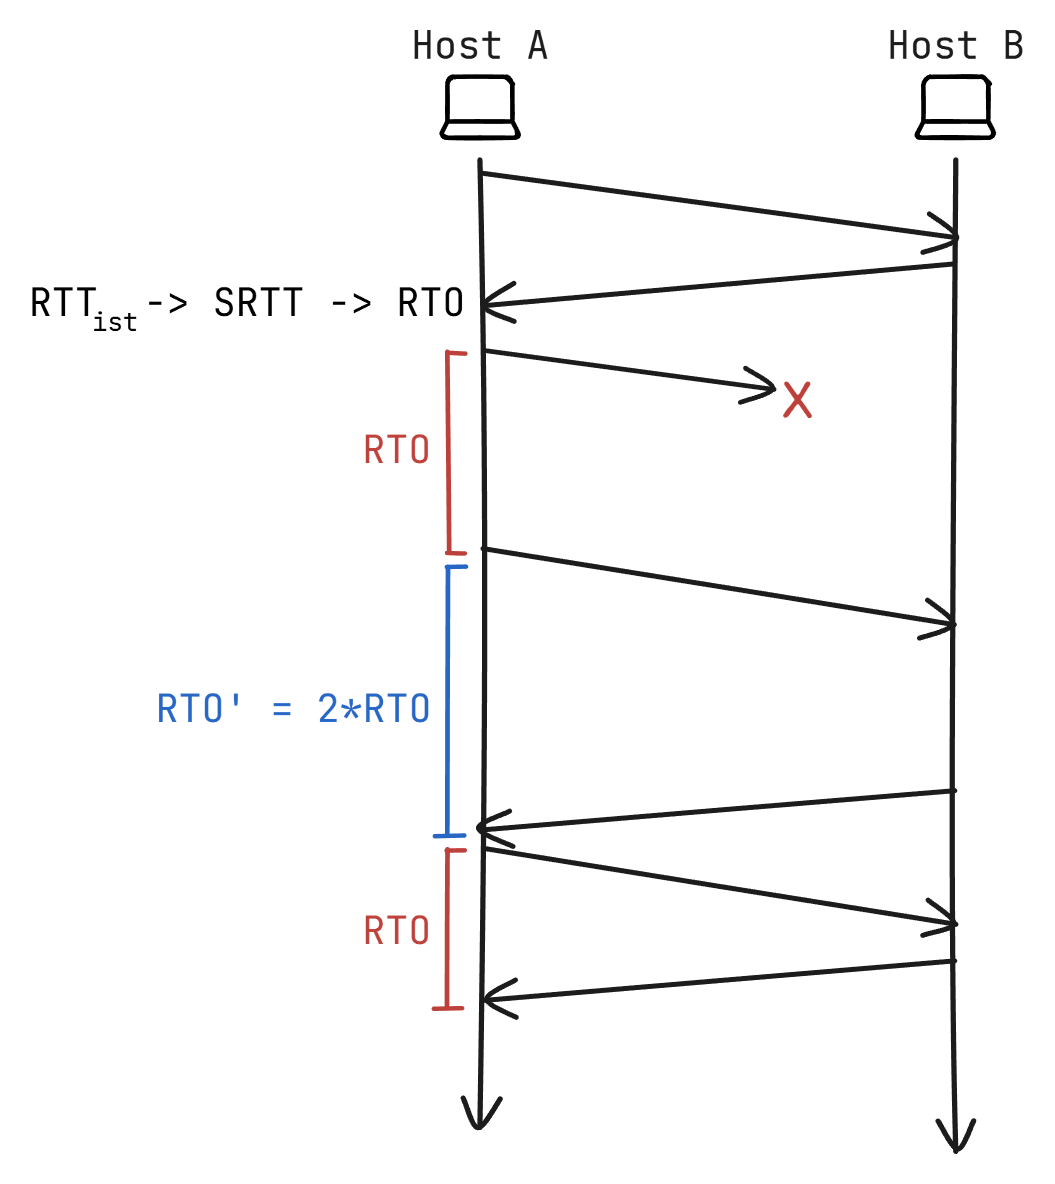
\includegraphics[width=0.7\textwidth]{rto-doppio}
  \caption{Esempio del raddoppio dell'RTO}
\end{figure}

\noindent 
Se si inviasse un segmento ad ogni RTT, la velocità di trasmissione sarebbe:
\[
  \frac{1segm}{RTT}
\]
Quindi se un segmento è di \( 1500byte \) e un RTT è di \( 10ms \), allora la velocità
di trasmissione sarebbe:
\[
  \frac{1500byte}{10ms} = 120Kbit/s
\]

\subsubsection{Velocità di trasmissione}
Invece di trasmettere un singolo segmento ad ogni RTT, se ne trasmettono di più
contemporaneamente.
\begin{figure}[H]
  \centering
  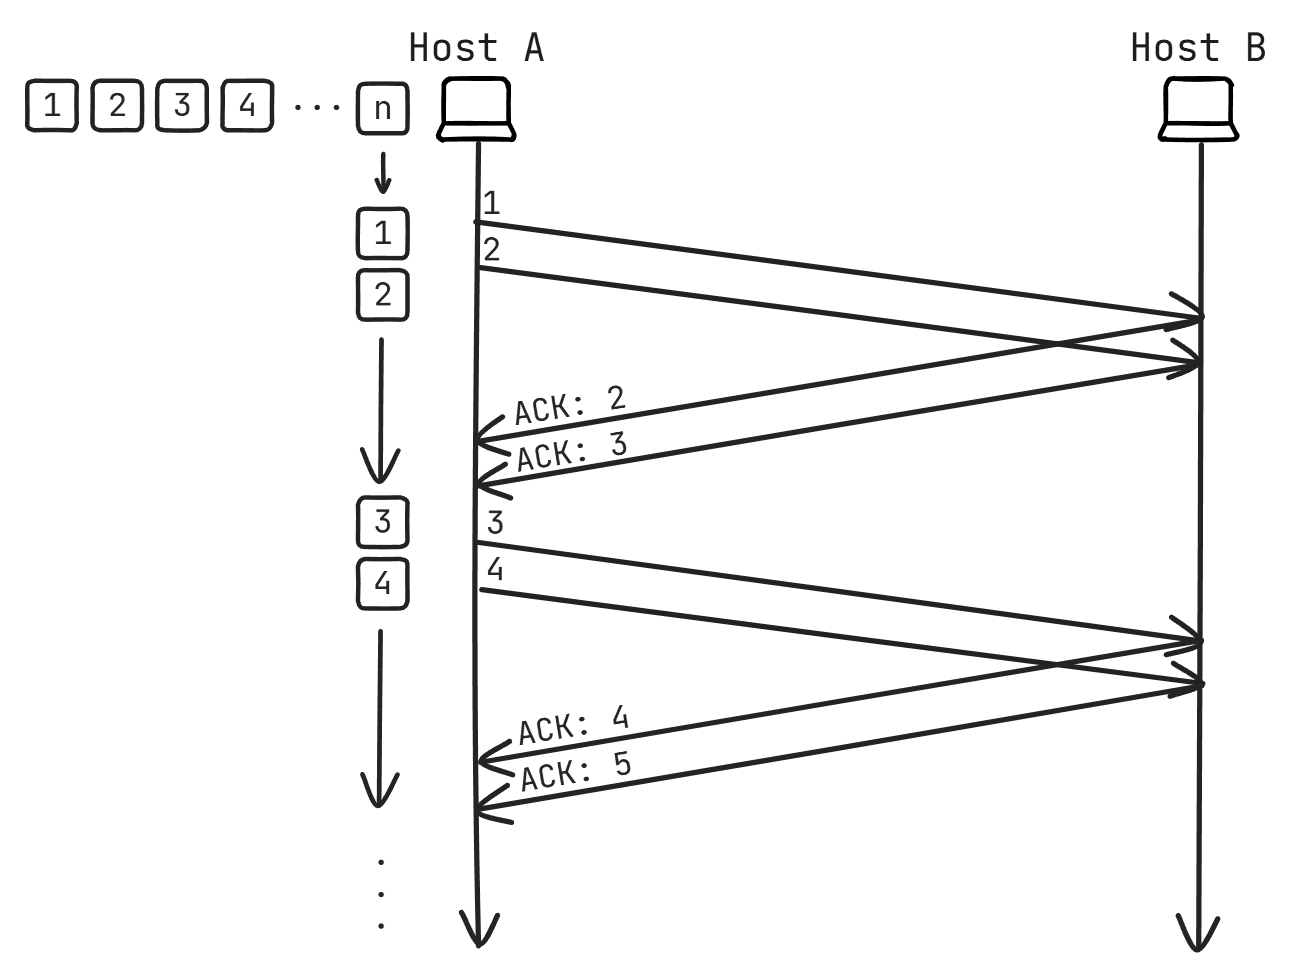
\includegraphics[width=0.7\textwidth]{doppio-pacchetto}
  \caption{Invio di più segmenti contemporaneamente}
\end{figure}

\noindent
Consideriamo la congestione come la perdita di un segmento, cioè un riscontro non
ricevuto.
\begin{itemize}
  \item \textbf{Controllo di flusso}: È un'azione preventiva per limitare la congestione
    \begin{itemize}
      \item 
        Quanti segmenti contemporaneamente? 
      \item 
        Come gestisco i riscontri? 
    \end{itemize}

  \item \textbf{Controllo di congestione}: È una reazione in caso di congestione
    \begin{itemize}
      \item 
        Cosa succede se uno dei segmenti viene perso (e gli altri no)? 
    \end{itemize}
\end{itemize}

\subsubsection{Controllo di flusso}
Il controllo di flusso è un meccanismo che invia più segmenti contemporaneamente con un
meccanismo a \textbf{finestra scorrevole} (sliding window):
\begin{figure}[H]
  \centering
  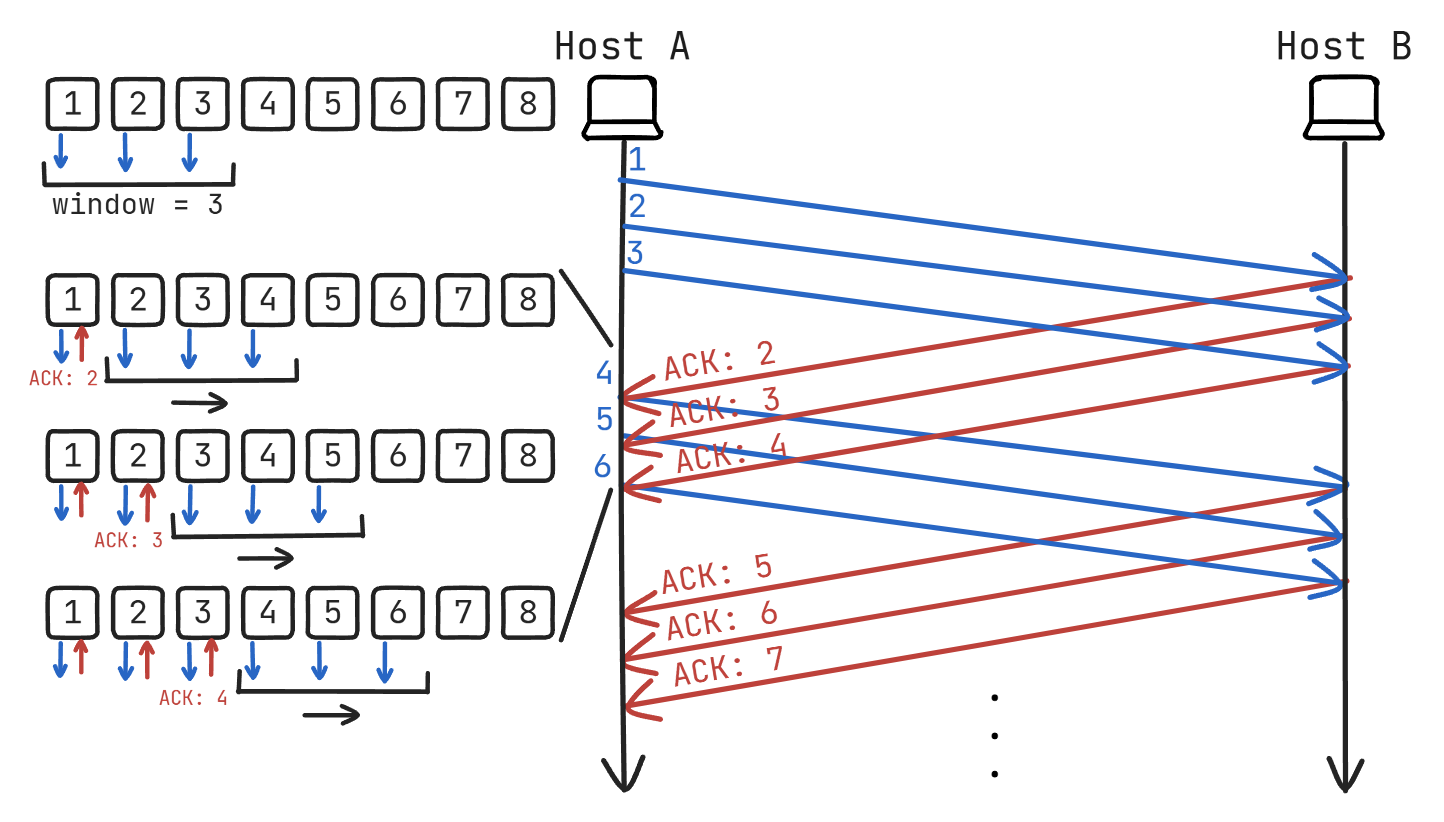
\includegraphics[width=1\textwidth]{sliding-window}
  \caption{Esempio di finestra scorrevole}
\end{figure}
\noindent
Questo meccanismo prevede che si salvino i segmenti inviati e si aspettino i riscontri
per poter inviare i segmenti successivi. Se \( w \) è il numero di segmenti da inviare,
allora ad ogni RTT si invieranno:
\[
\frac{w\,segmenti}{RTT}
\] 

\subsubsection{Controllo di congestione}
In caso di perdita di un segmento, la finestra non scorre più perchè il riscontro del
segmento perso non arriva, quindi bisogna aspettare il RTO e quando scade si ritrasmette
il segmento perso. Nel frattempo l'host che non ha ricevuto il segmento manda più ACK
in cui chiede di ritrasmettere il segmento perso (\textbf{ACK duplicati}). L'invio del singolo segmento chè
è stato perso è chiamato \textbf{Selective Repeat}. Le informazioni dei pacchetti non
ricevuti sono contenute nell'header TCP nel campo delle opzioni.
\begin{figure}[H]
  \centering
  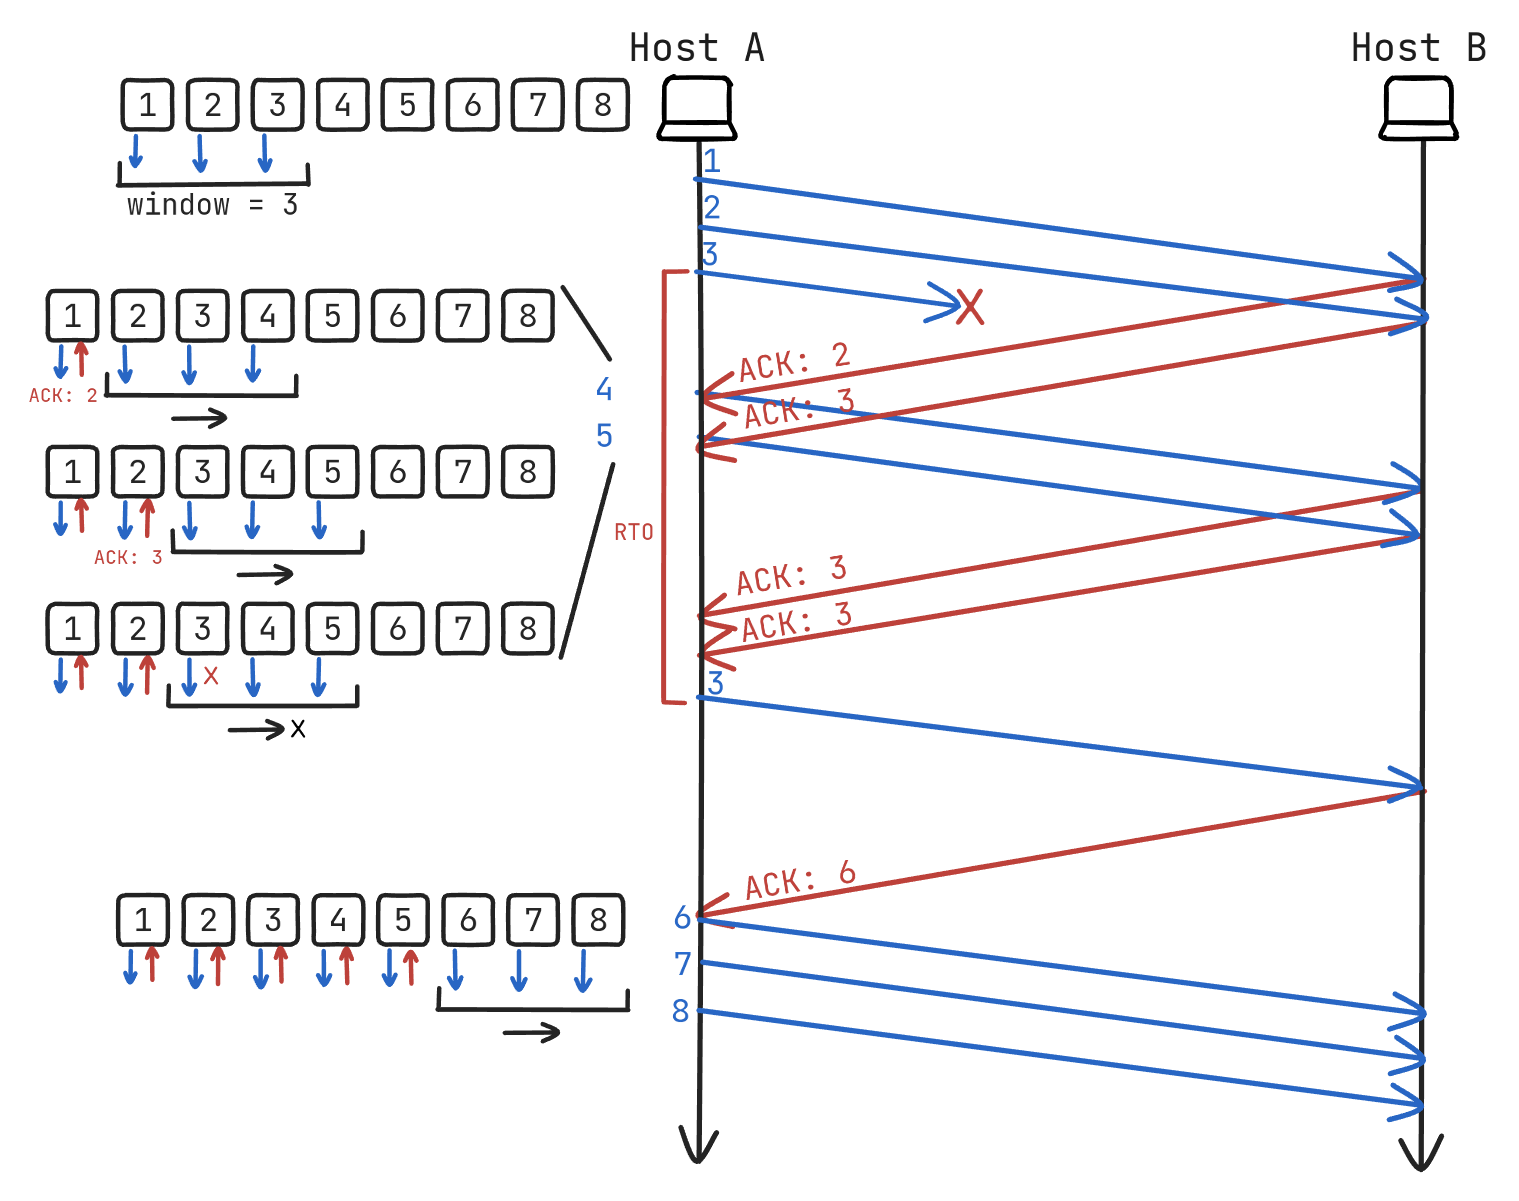
\includegraphics[width=1\textwidth]{selective-repeat}
  \caption{Selective Repeat}
\end{figure}

\noindent
Lo scorrimento della finestra viene impedito anche se la ricezione dei segmenti avviene
in ordine diverso da quello di invio.
\begin{figure}[H]
  \centering
  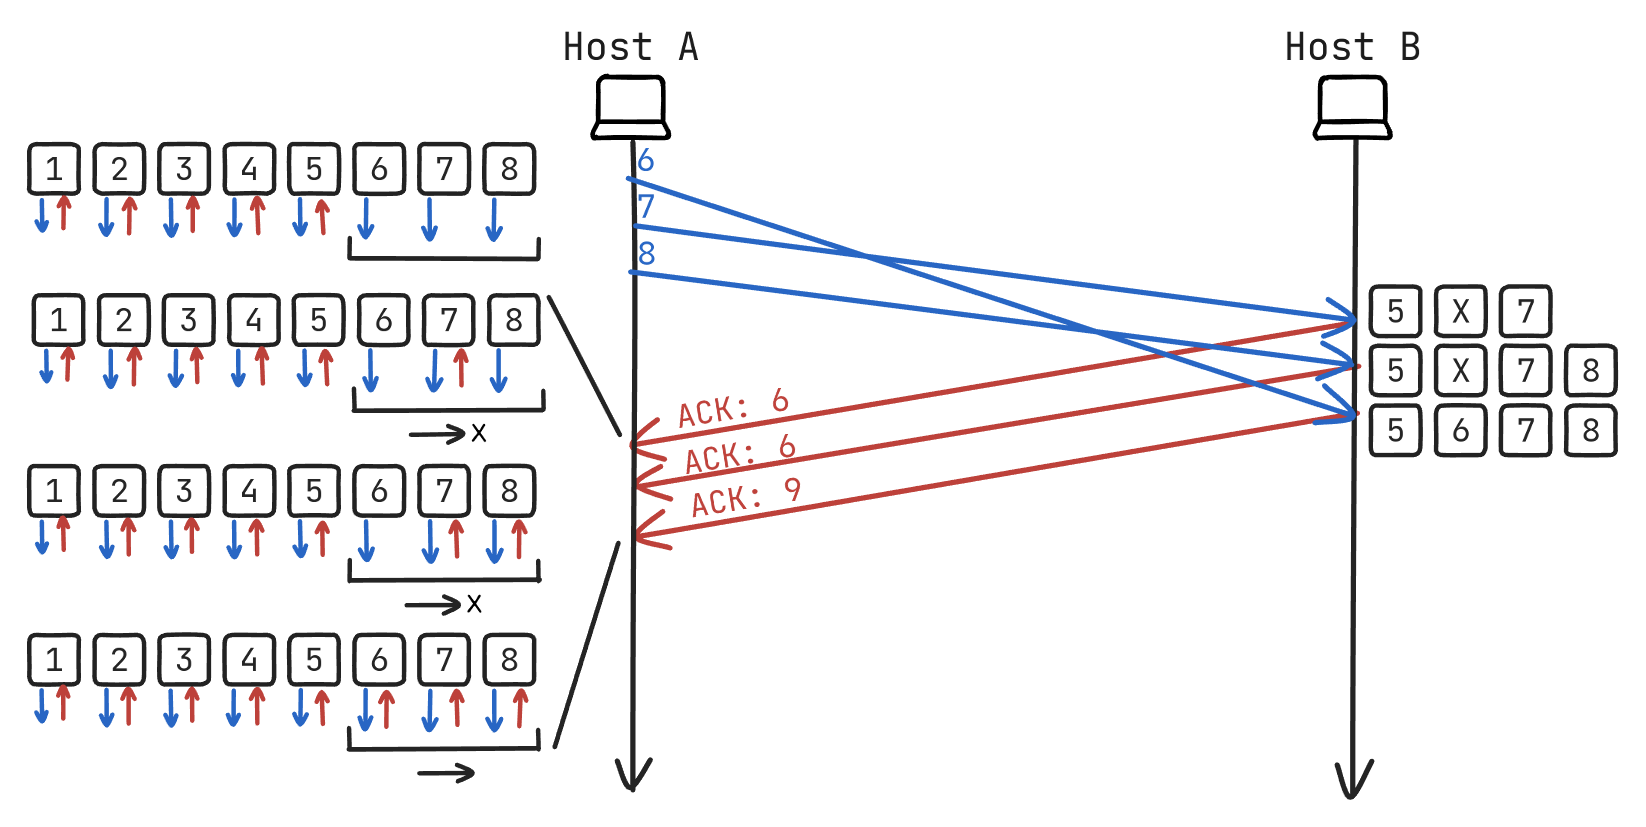
\includegraphics[width=1\textwidth]{selective-repeat-disordinato}
  \caption{Selective Repeat con segmenti disordinati}
\end{figure}

\noindent
Se un router riceve tanti pacchetti di fila che non entrano nel buffer, adotta una
politica secondo cui scarta dei pacchetti a caso dal buffer per fare spazio ai nuovi 
pacchetti.

\subsubsection{Finestra di trasmissione}
L'unico segnale per determinare la dimensione della finestra è il riscontro, quindi
si utilizzano i riscontri (o la loro assenza) per variare in maniera dinamica la
grandezza della finestra. 
\begin{figure}[H]
  \centering
  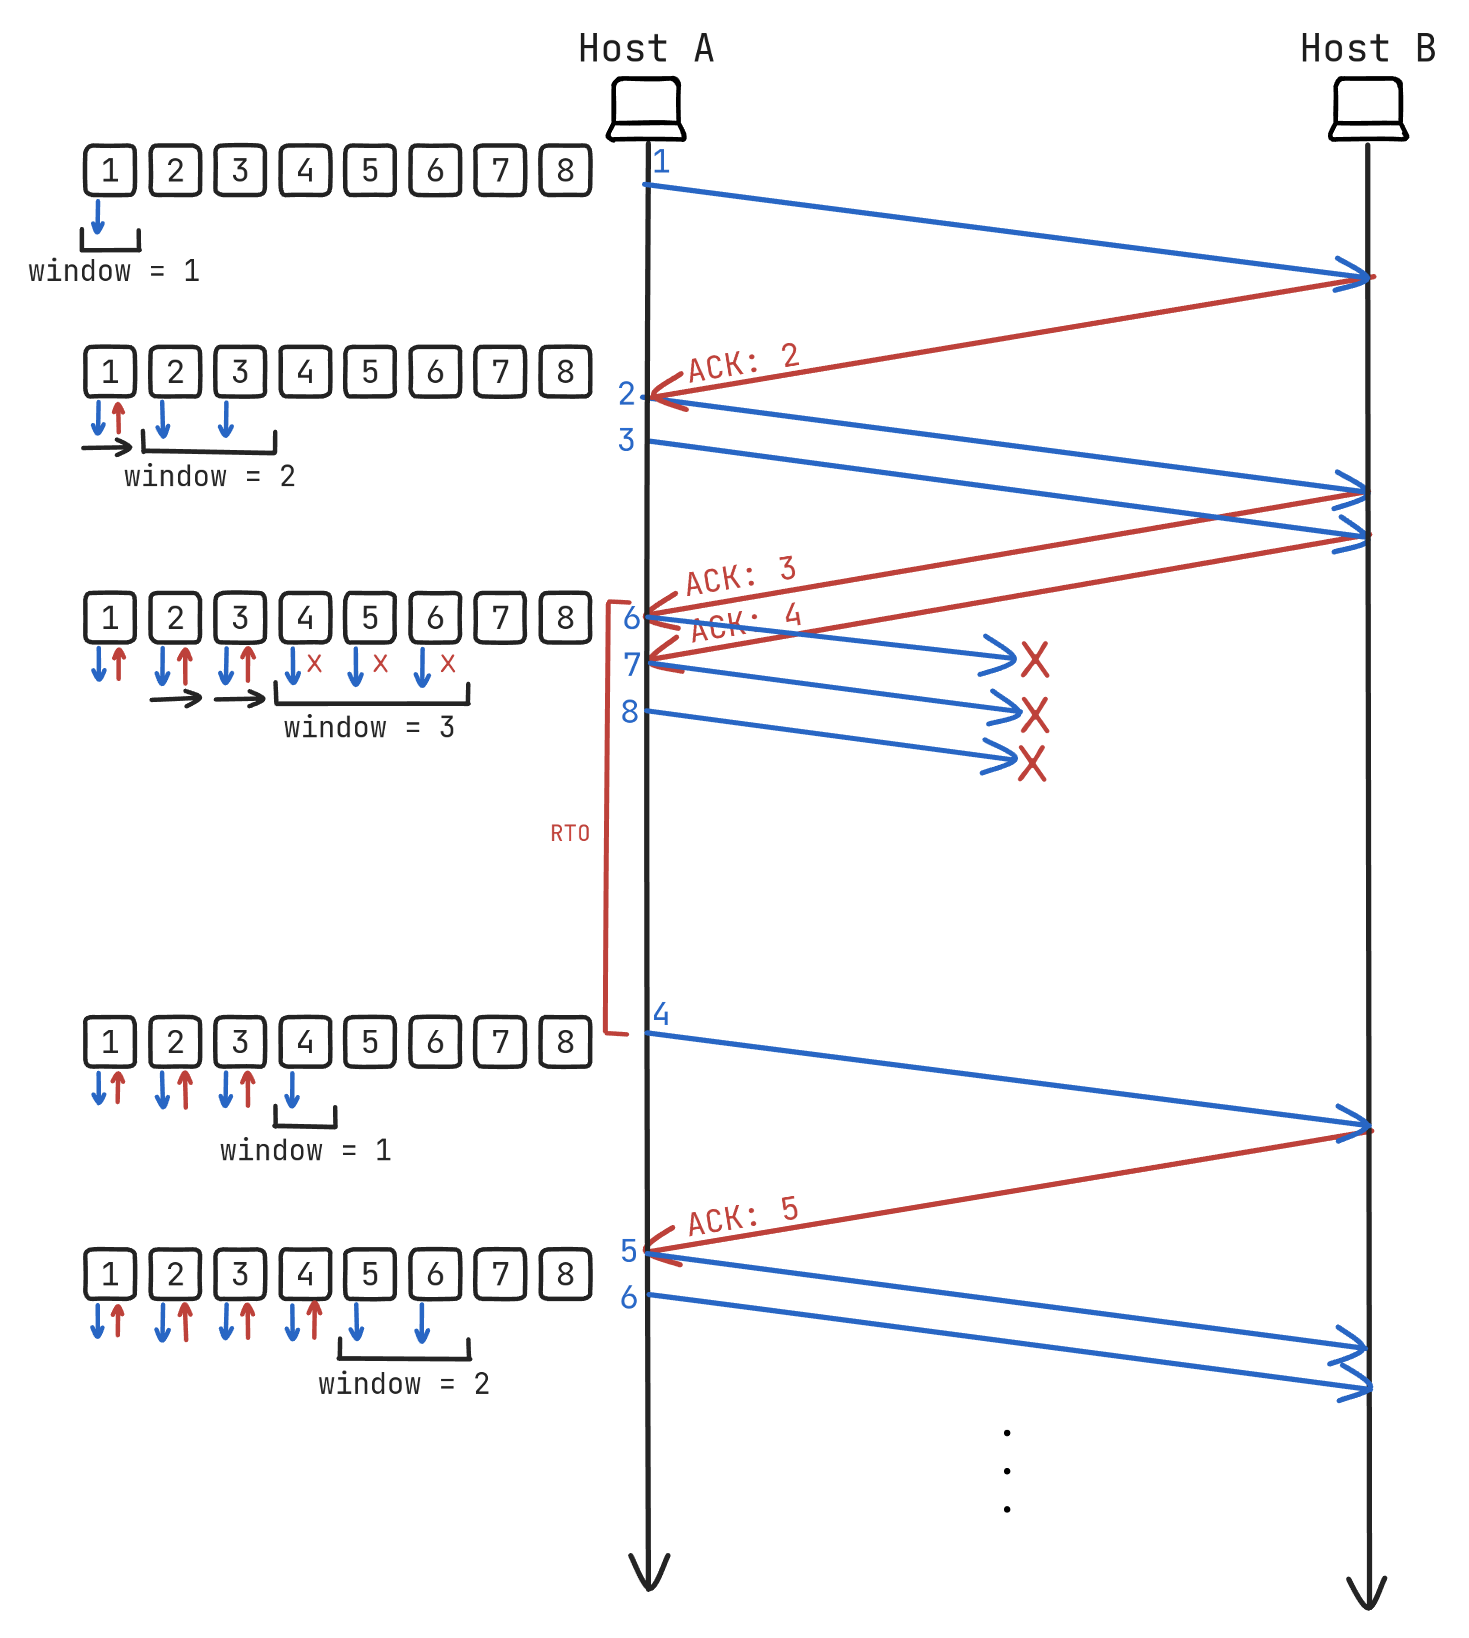
\includegraphics[width=1\textwidth]{finestra-dinamica}
  \caption{Dimensione dinamica della finestra}
\end{figure}
\begin{itemize}
  \item \textbf{Riscontri positivi regolari}: Si può aumentare la dimensione della
    finestra. Ci sono 2 possibilità di aumento della finestre:
    \begin{enumerate}
      \item \textbf{Slow start}: Per ogni riscontro ricevuto, si fa scorrere la finestra
        verso destra di un segmento e si aumenta la sua dimensione di un segmento
        \begin{figure}[H]
          \centering
          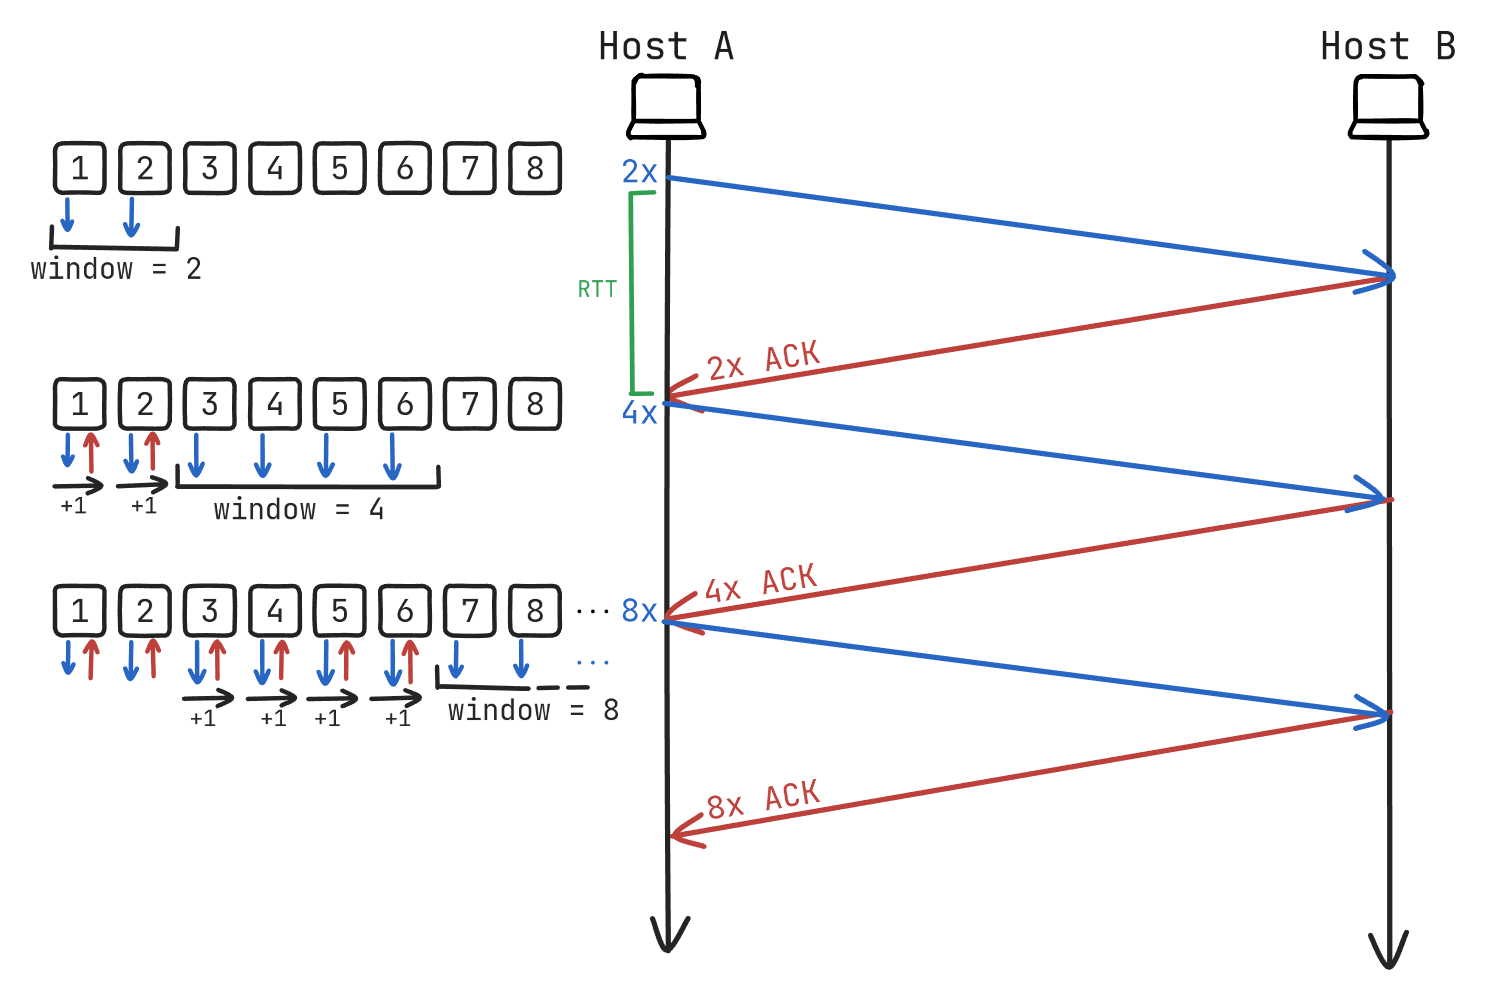
\includegraphics[width=0.8\textwidth]{slow-start}
          \caption{Esempio Slow start}
        \end{figure}

        \noindent
        Il grafico della crescita della finestra è esponenziale:
        \begin{figure}[H]
          \centering
          \begin{tikzpicture}
            \draw[->] (0,-0.2) -- (0,4.5) node[left] {\( w \)};
            \draw[->] (-0.2,0) -- (4.5,0) node[below] {\( t \)};

            \fill[red] (1,0.5) circle (0.05);
            \fill[red] (2,1) circle (0.05);
            \fill[red] (3,2) circle (0.05);
            \fill[red] (4,4) circle (0.05);

            \draw[red,domain=1:4] plot (\x,{2^(\x-2)});

            \foreach \x in {1,2,3,4}
              \draw (\x,-0.1) -- (\x,0.1);

            \foreach \y in {1,2,4,8}
              \draw (-0.1,\y/2) -- (0.1,\y/2) node[left=0.2] {\y};

            \draw[green!50!black] (0.05,-0.2) -- ++(0,-0.2) -- ++(0.95,0)
              node[midway,below] {RTT} -- ++(0,0.2);
          \end{tikzpicture}
          \caption{Grafico Slow start}
        \end{figure}

      \item \textbf{Congestion avoidance}: Per ogni riscontro ricevuto, si aumenta
        la finestra di \( \frac{1}{w} \) dove \( w \) è la dimensione della finestra
        precedente.
        \begin{figure}[H]
          \centering
          \includegraphics[width=0.8\textwidth]{congestion-avoidance}
          \caption{Esempio Congestion avoidance}
        \end{figure}

        \noindent
        Il grafico della crescita della finestra è lineare:
        \begin{figure}[H]
          \centering
          \begin{tikzpicture}
            \draw[->] (0,-0.2) -- (0,4.5) node[left] {\( w \)};
            \draw[->] (-0.2,0) -- (4.5,0) node[below] {\( t \)};

            \fill[red] (1,1) circle (0.05);
            \fill[red] (2,2) circle (0.05);
            \fill[red] (3,3) circle (0.05);
            \fill[red] (4,4) circle (0.05);

            \draw[red] (1,1) -- (4,4);

            \foreach \x in {1,2,3,4}
              \draw (\x,-0.1) -- (\x,0.1);

            \foreach \y in {2,3,4,5}
              \draw (-0.1,\y-1) -- (0.1,\y-1) node[left=0.2] {\y};

            \draw[green!50!black] (0.05,-0.2) -- ++(0,-0.2) -- ++(0.95,0)
              node[midway,below] {RTT} -- ++(0,0.2);
          \end{tikzpicture}
        \end{figure}
    \end{enumerate}
  \item \textbf{In caso di perdite}: Il RTO scade, si ritrasmette il segmento perso
    e si riduce la dimensione della finestra. Ci sono 2 possibilità di riduzione della
    finestra:
    \begin{enumerate}
      \item \textbf{Vanilla}: Una volta scaduto il RTO si riduce la finestra a 1 e si 
        ritrasmettono i segmenti persi.

      \item \textbf{Fast retrasmit/Fast recovery}: In caso di ricezione di 3 ACK duplicati
        di seguito, si pone la finestra a \( \frac{w}{2} \) e si ritrasmette il segmento
        indicato negli ACK duplicati (se ci sono delle opzioni nell'header che indicano
        altri segmenti mancanti si ritrasmettono anche quelli).
        \begin{figure}[H]
          \centering
          \includegraphics[width=1\textwidth]{fast-retrasmit-fast-recovery}
          \caption{Esempio Fast retrasmit/Fast recovery}
        \end{figure}
    \end{enumerate}
\end{itemize}

\noindent
L'algoritmo di controllo della congestione è il seguente:
\begin{itemize}
  \item \textbf{Variabili}:
    \begin{enumerate}
      \item \texttt{cwnd}: Congestion Window, è la dimensione della finestra di
        trasmissione attuale
      \item \texttt{rto}: Calcolato dinamicamente in base all'RTT istantaneo e SRTT
      \item \texttt{rcvwnd}: Recieve Window, è la finestra massima di ricezione
      \item \texttt{ssthresh}: Slow Start Threshold, è una soglia usata per distinguere
        l'uso dell'algoritmo slow start o congestion avoidance
    \end{enumerate}

  \item \textbf{Inizializzazione}: All'inizio della connessione non si sanno tante
    informazioni, quindi si pongono le variabili nel modo più "conservativo" possibile:
    \begin{enumerate}
      \item \texttt{cwnd} = 1
      \item \texttt{rto} = in base al valore dell'RTT misurato nel 3-way handshake
      \item \texttt{rcvwnd} = viene comunicato dalla destinazione in ogni riscontro
        nel campo \textbf{window}
      \item \texttt{ssthresh} = \texttt{rcvwnd} (in alcune implementazioni è 
        \( \frac{rcvwnd}{2} \))
    \end{enumerate}

  \item \textbf{Algoritmo}:
    \begin{enumerate}
      \item Invia un numero di segmenti pari alla \texttt{cwnd}
      \item Quando arrivano i riscontri:
        \begin{lstlisting}[language=Scala]
if cwnd < ssthresh // Uso lo slow start
  cwnd = min(cwnd + numAck, rcvwnd, ssthresh)
else // Uso il congestion avoidance
  cwnd = min(cwnd + numAck / cwnd, rcvwnd)

// Torno al punto 1
        \end{lstlisting}

      \item Se non arrivano i riscontri (quando scade il RTO):
        \begin{enumerate}
          \item 
            Pongo la \texttt{ssthresh} = \( \frac{\texttt{cwnd}}{2} \) (\texttt{cwnd} al momento della
            perdita)
          \item Pongo la \texttt{cwnd} = 1 (Vanilla tcp)
          \item Per i segmenti ritrasmessi pongo la \texttt{rto} = 2 \texttt{rto} 
          \item Torno al punto 1.
        \end{enumerate}
    \end{enumerate}
\end{itemize}

\begin{example}
  Un esempio (semplificato in cui RTT è stabile) di evoluzione della trasmissione con TCP
  è il seguente:
  \begin{figure}[H]
    \centering
    \includegraphics[width=1\textwidth]{cwnd}
    \caption{Evoluzione della finestra di trasmissione}
  \end{figure}
  \noindent 
  Il grafico del cambio della dimensione della finestra è il seguente:
  \begin{figure}[H]
    \centering
    \begin{tikzpicture}
      \draw[->] (0,-0.2) -- (0,4.5) node[left] {\( w \)};
      \draw[->] (-0.2,0) -- (9.5,0) node[below] {\( t \)};

      % rcvwnd & ssthresh
      \draw[red] (0,8/2) node[above right] {\texttt{rcvwnd = 8}} -- (9.5,8/2);
      \draw[orange] (0,4/2) node[above right] {\texttt{ssthresh = 4}} -- (6,4/2)
        -- (6,3/2) -- (9.5,3/2);

      \fill[blue] (0,1/2) circle (0.05);
      \fill[blue] (1,2/2) circle (0.05);
      \fill[blue] (2,4/2) circle (0.05);
      \fill[blue] (3,5/2) circle (0.05);
      \fill[blue] (4,6/2) circle (0.05) node[right,red] {\( \times \)};

      % Loss
      \draw[purple,dashed] (4.5,6/2) -- (6,6/2) -- (6,1/2);

      \fill[blue] (6,1/2) circle (0.05);
      \fill[blue] (7,2/2) circle (0.05);
      \fill[blue] (8,3/2) circle (0.05);
      \fill[blue] (9,4/2) circle (0.05);

      % Functions
      \draw[blue,domain=0:2] plot (\x,{2^(\x-1)});
      \draw[blue] (2,4/2) -- (4,6/2);

      \draw[blue,domain=6:7] plot (\x,{2^(\x-7)});
      \draw[blue] (7,2/2) -- (9,4/2);

      % Ticks
      \foreach \x in {1,2,3,4,5,6,7,8,9}
      \draw (\x,-0.1) -- (\x,0.1);

      \foreach \y in {1,2,4,8}
      \draw (-0.1,\y/2) -- (0.1,\y/2) node[left=0.2] {\y};

      \draw[green!50!black] (0.05,-0.2) -- ++(0,-0.2) -- ++(0.95,0)
        node[midway,below] {RTT} -- ++(0,0.2);
    \end{tikzpicture}
    \caption{Grafico Slow start}
  \end{figure}

  \noindent
  Nel lungo termine, con numeri più grandi, il comportamento della finestra sarà:
  \begin{figure}[H]
    \centering
    \begin{tikzpicture}
      \draw[->] (0,-0.2) -- (0,4.5) node[left] {\( w \)};
      \draw[->] (-0.2,0) -- (9.5,0) node[below] {\( t \)};

      \draw[blue,domain=0:4,scale=0.5] plot (\x,{2^(\x-2)});
      \draw[blue,domain=4:8,scale=0.5] plot (\x,{\x});
      \draw[scale=0.5,purple,dashed] (8,8) -- (9,8) -- (9,1/4);

      \draw[blue,domain=9:13,scale=0.5] plot (\x,{2^(\x-2-9)});
      \draw[blue,domain=13:16,scale=0.5] plot (\x,{\x-9});
      \draw[scale=0.5,purple,dashed] (16,7) -- (17,7) -- (17,1/4);
    \end{tikzpicture}
    \caption{Andamento Vanilla}
  \end{figure}
  \begin{figure}[H]
    \centering
    \begin{tikzpicture}
      \draw[->] (0,-0.2) -- (0,4.5) node[left] {\( w \)};
      \draw[->] (-0.2,0) -- (9.5,0) node[below] {\( t \)};

      \draw[blue,domain=0:4,scale=0.5] plot (\x,{2^(\x-2)});
      \draw[blue,domain=4:8,scale=0.5] plot (\x,{\x});
      \draw[scale=0.5,purple,dashed] (8,8) -- (9,8) -- (9,4);

      \draw[blue,domain=9:12,scale=0.5] plot (\x,{\x-5});
      \draw[scale=0.5,purple,dashed] (12,7) -- (13,7) -- (13,3);

      \draw[blue,domain=13:18,scale=0.5] plot (\x,{\x-10});
      \draw[scale=0.5,purple,dashed] (18,8) -- (19,8) -- (19,4);
    \end{tikzpicture}
    \caption{Andamento Fast retrasmit/Fast recovery}
  \end{figure}
\end{example}

\subsection{Protocollo UDP (User Datagram Protocol)}
Il protocollo UDP è un protocollo \textbf{connectionless}, cioè non c'è uno scambio
preliminare prima di inviare i dati, ed è anche \textbf{non affidabile}, cioè
se i segmenti vengono persi non vengono ritrasmessi.

\subsubsection{Formato del pacchetto}
La grandezza dell'header UDP è di \( 8 byte \) tutti scritti in 2 righe da 4 byte. I
campi dell'header sono i seguenti:
\begin{figure}[H]
  \centering
  \begin{tikzpicture}
    \def\len{7}
    \def\hei{0.8}

    \draw (0,0) rectangle ++(\len/2,-\hei) node[midway] {Porta sorgente};
    \draw (\len/2,0) rectangle ++(\len/2,-\hei) node[midway] {Porta destinazione};

    \draw (0,-\hei) rectangle ++(\len/2,-\hei) node[midway] {Lunghezza};
    \draw (\len/2,-\hei) rectangle ++(\len/2,-\hei) node[midway] {Checksum};

    \draw[fill,fill opacity=0.1,text opacity=1] (0,-\hei*2) rectangle ++(\len,-\hei*2) node[midway] {Dati};

    \node[above,scale=0.7] at (0,0) {0};
    \node[above,scale=0.7] at (\len/2,0) {15};
    \node[above,scale=0.7] at (\len,0) {31};
  \end{tikzpicture}
  \caption{Formato del pacchetto UDP}
\end{figure}

\begin{itemize}
  \item \textbf{Porta sorgente/destinazione}: Sono gli stessi campi presenti anche nel
    pacchetto TCP.

  \item \textbf{Lunghezza}: Indica la lunghezza del segmento UDP, cioè la somma della
    lunghezza dell'header e dei dati.

  \item \textbf{Checksum}: Serve per controllare la presenza di errori nel segmento.
    Bisogna avere un modo per capire se ci sono stati degli errori nella trasmissione dei
    dati per poter scartare il pacchetto.
\end{itemize}
Siccome UDP non ha il sequence number, sta all'applicazione che utilizza UDP gestire
come ordinare i pacchetti.


\section{Livello di rete}
\subsection{Protocollo IP (Internet Protocol)}
\subsubsection{Formato del pacchetto}
Il formato del pacchetto IP è il seguente:
\begin{figure}[H]
  \centering
  \begin{tikzpicture}
    \def\len{0.95*\linewidth}
    \def\hei{0.8}

    \draw (0,0) rectangle ++(\len/8,-\hei) node[midway] {Versione};
    \draw (\len/8,0) rectangle ++(\len/8,-\hei) node[midway,scale=0.7] {Header len.};
    \draw (\len/4,0) rectangle ++(\len/4,-\hei) node[midway] {Service type};
    \draw (\len/2,0) rectangle ++(\len/2,-\hei) node[midway] {Total length};

    \draw (0,-\hei) rectangle ++(\len/2,-\hei) node[midway] {Identification};
    \draw (\len/2,-\hei) rectangle ++(\len/10,-\hei) node[midway] {Flags};
    \draw (\len/10+\len/2,-\hei) rectangle ++(\len/2.5,-\hei) node[midway] {Fragment offset};

    \draw (0,-\hei*2) rectangle ++(\len/4,-\hei) node[midway] {TTL};
    \draw (\len/4,-\hei*2) rectangle ++(\len/4,-\hei) node[midway] {Type};
    \draw (\len/2,-\hei*2) rectangle ++(\len/2,-\hei) node[midway] {Header checksum};

    \draw (0,-\hei*3) rectangle ++(\len,-\hei) node[midway,scale=0.9] {Indirizzo IP sorgente};

    \draw (0,-\hei*4) rectangle ++(\len,-\hei) node[midway,scale=0.9] {Indirizzo IP destinazione};

    \draw (0,-\hei*5) rectangle ++(\len,-\hei) node[midway,scale=0.9] {Opzioni};

    \draw[fill,fill opacity=0.1,text opacity=1] (0,-\hei*6) rectangle ++(\len,-\hei*2) node[midway] {Dati};

    \node[above,scale=0.7] at (0,0) {0};
    \node[above,scale=0.7] at (\len/2,0) {15};
    \node[above,scale=0.7] at (\len,0) {31};
  \end{tikzpicture}
  \caption{Formato del pacchetto IP}
\end{figure}

\begin{itemize}
  \item \textbf{Versione} (4 bit): Indica la versione del protocollo IP utilizzato. Attualmente
    si utilizza la versione 4 (IPv4), la versione 6 (IPv6) è già implementata ma non
    ancora diffusa. Questo campo è stato pensato per poter supportare più versioni,
    siccome non si sapeva se il protocollo sarebbe stato utilizzato per molto tempo.

  \item \textbf{Lunghezza dell'header} (4 bit): Indica la lunghezza dell'header,
    che di solito è di 20 bit, ma può essere più lungo se ci sono delle opzioni.

  \item \textbf{Service type} (8 bit): È un codice che identifica una classe di servizio,
    cioè, come vengono gestiti i pacchetti nei buffer, ad esempio possono esserci
    delle priorità diverse per ogni buffer.

  \item \textbf{Lunghezza totale} (16 bit): Indica la lunghezza totale del pacchetto,
    cioè la somma della lunghezza dell'header e dei dati.

  \item \textbf{Identification} (16 bit): È un numero progressivo dato dalla sorgente
    (livello di rete) ad ogni pacchetto (non ha nessuna relazione con il numero di
    sequenza del TCP).
    Questo campo è utilizzato per il riassemblaggio dei pacchetti.

  \item \textbf{Flags} (3 bit): Sono dei bit che indicano se il pacchetto è frammentato
    o meno.

  \item \textbf{Fragment Offset} (13 bit): Indica l'offset del frammento rispetto al
    pacchetto originale (diviso per 8).

  \item \textbf{TTL (Time To Live)} (8 bit): È un contatore inizializzato dalla sorgente,
    che di solito vale 64 o 128, che indica il numero massimo di router che
    il pacchetto può attraversare, quindi ogni router che elabora tale pacchetto decrementa
    tale valore di 1, e se il valore diventa 0, il router scarta il pacchetto e manda un
    messaggio di errore alla sorgente.

    \vspace{1em}
    \noindent
    In caso di problemi, la rete deve ricalcolare i percorsi e nel frattempo si possono
    creare dei \textbf{routing-loop} (momentanei). Il TTL permette di non caricare la rete
    in caso di routing-loop.

  \item \textbf{Type} (8 bit): È un codice che identifica il protocollo usato nei
    dati trasportati nel payload.
    \begin{figure}[H]
      \centering
      \begin{tikzpicture}
        \draw[red] (0,0) rectangle ++(1,1);
        \draw[purple] (0.1,0.1) rectangle ++(0.3,0.3);

        \node[red,below,scale=0.8,align=center] at (0.5,0) {Header\\IP};
        \node[blue,above,scale=0.8,align=center] at (1.5,1) {Header\\trasporto};
        \node[purple,above,scale=0.5,align=center] at (0.25,0.4) {TCP};

        \draw[dashed,blue] (0,0) ++(1.1,0.1) rectangle ++(0.8,0.8);
        \draw (0,0) ++(1,0) rectangle ++(4,1);

        \draw (0,0) ++(1,-0.2) -- ++(0,-0.2) -- ++(4,0) node[midway,below] {Payload}
          -- ++(0,0.2);
      \end{tikzpicture}
      \caption{Type contiene il codice del protocollo di trasporto}
    \end{figure}

  \item \textbf{Header Checksum} (16 bit): Serve per controllare la presenza di errori
    nell'header del pacchetto.
\end{itemize}

\subsubsection{Frammentazione}
(Da non confondersi con la segmentazione del livello trasporto).
Data una tecnologia di trasmissione (scheda di rete, a livello data link) c'è una 
dimensione massima di trasmissione chiamata \textbf{MTU} (Maximum Transmission Unit).
\begin{figure}[H]
  \centering
  \includegraphics[width=0.7\textwidth]{mtu}
  \caption{Maximum Transmission Unit}
\end{figure}
\noindent
Se un pacchetto, durante il percorso, incontra un router che ha una MTU
minore di quella del pacchetto, il router \textbf{frammenta} il pacchetto in pacchetti
più piccoli con MTU compatibile con la linea di uscita.
Questo processo è chiamato \textbf{frammentazione}.
\begin{figure}[H]
  \centering
  \begin{tikzpicture}
    \draw[red] (0,0) rectangle ++(1,1) node[midway] {IP};
    \draw (0,0) ++(1,0) rectangle ++(4,1);

    \draw (0,1) ++(0,0.2) -- ++(0,0.2) -- ++(5,0) node[midway,above] {\( 1500byte \)}
      -- ++(0,-0.2);

    \draw[->] (2.5,0) -- ++(0,-1) node[midway,right,align=center] {Router con il link\\con \( MTU=1000byte \) }
      node[below] (f) {Frammentazione};

    \draw[->] (f) -- ++(-1,-1);
    \draw[red] (-2,-3.5) rectangle ++(1,1) node[midway] {IP};
    \draw (-2,-3.5) ++(1,0) rectangle ++(3,1);
    \draw (-2,-3.5) ++(0,-0.2) -- ++(0,-0.2) -- ++(4,0) node[midway,below] {\( 1000byte \)}
      -- ++(0,0.2);


    \draw[->] (f) -- ++(1,-1);
    \draw[red] (3,-3.5) rectangle ++(1,1) node[midway] {IP};
    \draw (3,-3.5) ++(1,0) rectangle ++(2,1);
    \draw (3,-3.5) ++(0,-0.2) -- ++(0,-0.2) -- ++(3,0) node[midway,below] {\( < 1000byte \)}
      -- ++(0,0.2);
  \end{tikzpicture}
  \caption{Esempio di frammentazione}
\end{figure}

\noindent
Solo l'host di destinazione (non il router della lan a cui appartiene l'host,
nè i router intermedi) è responsabile del riassemblaggio dei pacchetti.

Quando la destinazione riceve un frammento fa partire un timer (\( 250ms-500ms \)),
se non riceve tutti i frammenti entro la scadenza del timer, scarta tutti i frammenti,
altrimenti ricompone il pacchetto e lo consegna a livello di trasporto.

\vspace{1em}
\noindent
I campi dell'header IP coinvolti nella frammentazione sono:
\begin{itemize}
  \item \textbf{Identification}
  \item \textbf{Flags}
    \begin{itemize}
      \item Flag \( M \):
        \begin{itemize}
          \item 0: Se il pacchetto non è stato frammentato, oppure se è l'ultimo
            frammento
          \item 1: Se il pacchetto è un frammento, tranne l'ultimo
        \end{itemize}
    \end{itemize}
  \item \textbf{Fragment Offset}
\end{itemize}
\begin{example}
  Prendiamo ad esempio un pacchetto che ha come \( MTU = 5000 byte \) e genera un
  pacchetto di \( 4000 byte + 20 byte \) di header IP.
  \begin{figure}[H]
    \centering
    \begin{tikzpicture}
      \def\len{0.95*\linewidth}
      \def\hei{0.6}

      \draw (0,0) rectangle ++(\len/8,-\hei) node[midway] {};
      \draw (\len/8,0) rectangle ++(\len/8,-\hei) node[midway,scale=0.7] {};
      \draw (\len/4,0) rectangle ++(\len/4,-\hei) node[midway] {};
      \draw (\len/2,0) rectangle ++(\len/2,-\hei) node[midway] {};

      \draw (0,-\hei) rectangle ++(\len/2,-\hei) node[midway] {Identification = 476};
      \draw (\len/2,-\hei) rectangle ++(\len/10,-\hei) node[midway,scale=0.9] {M = 0};
      \draw (\len/10+\len/2,-\hei) rectangle ++(\len/2.5,-\hei) node[midway] {Offset = 0};

      \draw (0,-\hei*2) rectangle ++(\len/4,-\hei) node[midway] {};
      \draw (\len/4,-\hei*2) rectangle ++(\len/4,-\hei) node[midway] {};
      \draw (\len/2,-\hei*2) rectangle ++(\len/2,-\hei) node[midway] {};

      \draw (0,-\hei*3) rectangle ++(\len,-\hei) node[midway,scale=0.9] {Indirizzo IP sorgente};

      \draw (0,-\hei*4) rectangle ++(\len,-\hei) node[midway,scale=0.9] {Indirizzo IP destinazione};

      \draw (0,-\hei*5) rectangle ++(\len,-\hei) node[midway,scale=0.9] {};

      \draw[fill,fill opacity=0.1,text opacity=1] (0,-\hei*6) rectangle ++(\len,-\hei*2) node[midway] {Dati};

      \node[above,scale=0.7] at (0,0) {0};
      \node[above,scale=0.7] at (\len/2,0) {15};
      \node[above,scale=0.7] at (\len,0) {31};
    \end{tikzpicture}
    \caption{Pacchetto non frammentato}
  \end{figure}
  \noindent
  Durante il percorso il pacchetto passa attraverso un router con link di uscita con 
  \( MTU = 1420 byte\) (\( 1400 \) per il payload e \( 20 \) per l'header) 
  \begin{figure}[H]
    \centering
    \begin{tikzpicture}
      \def\len{0.25*\linewidth}
      \def\hei{0.6}

      \draw (0,0) rectangle ++(\len/8,-\hei) node[midway] {};
      \draw (\len/8,0) rectangle ++(\len/8,-\hei) node[midway,scale=0.7] {};
      \draw (\len/4,0) rectangle ++(\len/4,-\hei) node[midway] {};
      \draw (\len/2,0) rectangle ++(\len/2,-\hei) node[midway] {};

      \draw (0,-\hei) rectangle ++(\len/2,-\hei) node[midway] {476};
      \draw (\len/2,-\hei) rectangle ++(\len/10,-\hei) node[midway,scale=0.9] {1};
      \draw (\len/10+\len/2,-\hei) rectangle ++(\len/2.5,-\hei) node[midway] {0};

      \draw (0,-\hei*2) rectangle ++(\len/4,-\hei) node[midway] {};
      \draw (\len/4,-\hei*2) rectangle ++(\len/4,-\hei) node[midway] {};
      \draw (\len/2,-\hei*2) rectangle ++(\len/2,-\hei) node[midway] {};

      \draw (0,-\hei*3) rectangle ++(\len,-\hei) node[midway,scale=0.8] {IP sorgente};

      \draw (0,-\hei*4) rectangle ++(\len,-\hei) node[midway,scale=0.8] {IP destinazione};

      \draw (0,-\hei*5) rectangle ++(\len,-\hei) node[midway,scale=0.9] {};

      \draw[fill,fill opacity=0.1,text opacity=1] (0,-\hei*6) rectangle ++(\len,-\hei*2) node[midway] {Dati};

      \node[above,scale=0.7] at (0,0) {0};
      \node[above,scale=0.7] at (\len/2,0) {15};
      \node[above,scale=0.7] at (\len,0) {31};

      \draw (-0.1,-\hei*8) -- ++(-0.1,0) -- ++(0,\hei*2) node[midway,above,rotate=90,scale=0.8]
        {\( 1400\,byte \) } -- ++(0.1,0);
    \end{tikzpicture}
    \begin{tikzpicture}
      \def\len{0.25*\linewidth}
      \def\hei{0.6}

      \draw (0,0) rectangle ++(\len/8,-\hei) node[midway] {};
      \draw (\len/8,0) rectangle ++(\len/8,-\hei) node[midway,scale=0.7] {};
      \draw (\len/4,0) rectangle ++(\len/4,-\hei) node[midway] {};
      \draw (\len/2,0) rectangle ++(\len/2,-\hei) node[midway] {};

      \draw (0,-\hei) rectangle ++(\len/2,-\hei) node[midway] {476};
      \draw (\len/2,-\hei) rectangle ++(\len/10,-\hei) node[midway,scale=0.9] {1};
      \draw (\len/10+\len/2,-\hei) rectangle ++(\len/2.5,-\hei) node[midway] {175};

      \draw (0,-\hei*2) rectangle ++(\len/4,-\hei) node[midway] {};
      \draw (\len/4,-\hei*2) rectangle ++(\len/4,-\hei) node[midway] {};
      \draw (\len/2,-\hei*2) rectangle ++(\len/2,-\hei) node[midway] {};

      \draw (0,-\hei*3) rectangle ++(\len,-\hei) node[midway,scale=0.8] {IP sorgente};

      \draw (0,-\hei*4) rectangle ++(\len,-\hei) node[midway,scale=0.8] {IP destinazione};

      \draw (0,-\hei*5) rectangle ++(\len,-\hei) node[midway,scale=0.9] {};

      \draw[fill,fill opacity=0.1,text opacity=1] (0,-\hei*6) rectangle ++(\len,-\hei*2) node[midway] {Dati};

      \node[above,scale=0.7] at (0,0) {0};
      \node[above,scale=0.7] at (\len/2,0) {15};
      \node[above,scale=0.7] at (\len,0) {31};

      \draw (-0.1,-\hei*8) -- ++(-0.1,0) -- ++(0,\hei*2) node[midway,above,rotate=90,scale=0.8]
        {\( 1400\,byte \) } -- ++(0.1,0);
    \end{tikzpicture}
    \begin{tikzpicture}
      \def\len{0.25*\linewidth}
      \def\hei{0.6}

      \draw (0,0) rectangle ++(\len/8,-\hei) node[midway] {};
      \draw (\len/8,0) rectangle ++(\len/8,-\hei) node[midway,scale=0.7] {};
      \draw (\len/4,0) rectangle ++(\len/4,-\hei) node[midway] {};
      \draw (\len/2,0) rectangle ++(\len/2,-\hei) node[midway] {};

      \draw (0,-\hei) rectangle ++(\len/2,-\hei) node[midway] {476};
      \draw (\len/2,-\hei) rectangle ++(\len/10,-\hei) node[midway,scale=0.9] {0};
      \draw (\len/10+\len/2,-\hei) rectangle ++(\len/2.5,-\hei) node[midway] {350};

      \draw (0,-\hei*2) rectangle ++(\len/4,-\hei) node[midway] {};
      \draw (\len/4,-\hei*2) rectangle ++(\len/4,-\hei) node[midway] {};
      \draw (\len/2,-\hei*2) rectangle ++(\len/2,-\hei) node[midway] {};

      \draw (0,-\hei*3) rectangle ++(\len,-\hei) node[midway,scale=0.8] {IP sorgente};

      \draw (0,-\hei*4) rectangle ++(\len,-\hei) node[midway,scale=0.8] {IP destinazione};

      \draw (0,-\hei*5) rectangle ++(\len,-\hei) node[midway,scale=0.9] {};

      \draw[fill,fill opacity=0.1,text opacity=1] (0,-\hei*6) rectangle ++(\len,-\hei*2) node[midway] {Dati};

      \node[above,scale=0.7] at (0,0) {0};
      \node[above,scale=0.7] at (\len/2,0) {15};
      \node[above,scale=0.7] at (\len,0) {31};

      \draw (-0.1,-\hei*8) -- ++(-0.1,0) -- ++(0,\hei*2) node[midway,above,rotate=90,scale=0.8]
        {\( 1200\,byte \) } -- ++(0.1,0);
    \end{tikzpicture}

    \vspace{2em}
    \noindent
    \begin{tikzpicture}
      \draw[red] (0,0) rectangle ++(1,1) node[midway] {IP};
      \draw (0,0) ++(1,0) rectangle ++(8,1);

      \draw (0,1) ++(1,0.2) -- ++(0,0.2) -- ++(3,0) node[midway,above] {\( 1400byte \)}
        -- ++(0,-0.2);

      \draw (0,1) ++(4,0.2) -- ++(0,0.2) -- ++(3,0) node[midway,above] {\( 1400byte \)}
        -- ++(0,-0.2);

      \draw (0,1) ++(7,0.2) -- ++(0,0.2) -- ++(2,0) node[midway,above] {\( 1200byte \)}
        -- ++(0,-0.2);
    \end{tikzpicture}
    \caption{Pacchetto frammentato}
  \end{figure}

  \noindent
  Gli offset sono:
  \begin{itemize}
    \item Primo frammento: \( \frac{0}{8} = 0 \) 
    \item Secondo frammento: \( \frac{1400}{8} = 175 \) 
    \item Terzo frammento: \( \frac{2800}{8} = 350 \)
  \end{itemize}
\end{example}

\subsection{Routing/instradamento}
Un pacchetto potrebbe essere ovunque nella rete, quindi data la destinazione, il livello
di rete deve \textbf{fare il possibile} (servizio \textbf{best effort}) per consegnare il
pacchetto a tale destinazione.

Il \textbf{routing} è diviso in:
\begin{itemize}
  \item \textbf{Consegna diretta}: La consegna di un pacchetto dall'host \( A \) all'host
    \( B \) è diretta e non passa per nessun router:
    \begin{figure}[H]
      \centering
      \includegraphics[width=0.8\textwidth]{consegna-diretta}
      \caption{Consegna diretta}
    \end{figure}

  \item \textbf{Consegna indiretta}: La consegna di un pacchetto dall'host \( A \) all'host
    \( C \) è indiretta e passa per uno o più router:
    \begin{figure}[H]
      \centering
      \includegraphics[width=0.8\textwidth]{consegna-indiretta}
      \caption{Consegna indiretta}
    \end{figure}
\end{itemize}
Un host conosce, oltre al proprio indirizzo IP, la maschera della rete a cui appartiene
e conosce l'indirizzo IP del router di bordo della rete a cui appartiene:
\begin{figure}[H]
  \centering
  \includegraphics[width=0.3\textwidth]{indirizzo-interfaccia}
  \caption{Indirizzo delle interfacce di un router}
\end{figure}

\noindent
Data una destinazione \( \left( IP_D \right)  \) l'host confronta:
\[
  IP \;\& \;\text{Maschera} = IP_{\text{Rete}_1}
\] 
con
\[
  IP_D \;\& \;\text{Maschera} = IP_{\text{Rete}_2}
\] 
\begin{itemize}
  \item 
    Se i due valori sono uguali, allora la destinazione appartiene alla stessa rete dell'host,
    di conseguenza si può fare la consegna diretta.

  \item 
    Se non lo sono, la destinazione appartiene ad un altra rete, quindi si deve fare la
    consegna indiretta delegando la consegna al router.
\end{itemize}

\begin{definition}
  Il routing è il processo di scoperta del cammino "migliore" da una sorgente a tutte
  le possibili destinazioni.
\end{definition}

\noindent
Un router tiene memorizzata una \textbf{tabella do routing} che contiene
\begin{itemize}
  \item \textbf{Indirizzo di destinazione}
  \item \textbf{Interfaccia di uscita}
  \item \textbf{Costo}
\end{itemize}
\begin{figure}[H]
  \centering
  \includegraphics[width=0.8\textwidth]{tabella-routing}
  \begin{tabular}{c|c|c}
    \textbf{Dst} & \textbf{Out} & \textbf{Costo} \\
    \hline
    \( IP_1 \) & \( A \) & \vdots \\
    \( IP_2 \) & \( B \) & \vdots \\
    \( IP_3 \) & \( C \) & \vdots \\
    \( \vdots \) & \( \vdots \) & \( \vdots \) \\
    \( IP_n \) & \( I_n \) & \( \vdots \)
  \end{tabular}
  \caption{Tabella di routing}
\end{figure}

\noindent
Il cammino migliore dipende dai criteri adottati da chi gestisce la rete (ISP).
Alcuni esempi di criteri sono:
\begin{itemize}
  \item 
    \textbf{Distanza} (cammino più corto) in termini di
    numero di \textbf{hop} (router attraversati), (tutti gli archi hanno peso = 1)

  \item \textbf{Numero di chilometri}

  \item \textbf{Velocità di trasmissione} (velocità nominale del link)
    \begin{figure}[H]
      \centering
      \includegraphics[width=0.5\textwidth]{velocita-trasmissione}
      \[
        T = \frac{B\,bit}{v}
      \]
      \caption{Velocità nominale del link}
    \end{figure}
    I pesi sono proporzionali all'inverso della banda.

  \item \textbf{Livello di congestione}
\end{itemize}
Questo processo viene astratto con l'utilizzo dei \textbf{grafi}:
\begin{figure}[H]
  \centering
  \includegraphics[width=0.8\textwidth]{grafo1}
  \caption{Diagramma di rete}
\end{figure}
\noindent
I router sono i \textbf{nodi} e i collegamenti sono gli \textbf{archi} del grafo:
\begin{figure}[H]
  \centering
  \includegraphics[width=0.8\textwidth]{grafo2}
  \caption{Grafo di rete}
\end{figure}
\noindent
Agli archi viene associato un numero detto \textbf{costo (o peso)} che caratterizza
l'arco stesso in base al criterio utilizzato.

\begin{definition}
  Il costo di un cammino tra un nodo \( i \) e un nodo \( j \) è la somma dei pesi degli
  archi che appartengono al cammino. Di conseguenza il routing è il calcolo del cammino
  a \textbf{costo minimo}.
\end{definition}

\subsubsection{Algoritmi per il calcolo dei cammini minimi}
Ad ogni algoritmo corrisponde un protocollo (diverso dal protocollo IP) che viene
trasportato dal protocollo IP. Periodicamente, ogni router, invia ai propri vicini
diretti un messaggio di aggiornamento (che cambia in base al tipo di algoritmo) che si 
distingue dagli altri messaggi, perchè nell'header IP c'è il campo \textbf{type}. Una
volta che un router riceve un messaggio di aggiornamento, aggiorna la propria tabella
di routing e inoltra il messaggio ai propri vicini, aggiornando così tutti i compomenti
della topologia della rete in caso di cambiamento.

\vspace{1em}
\noindent
Gli algoritmi per il calcolo del cammino minimo in un grafo sono di due tipi:
\begin{itemize}
  \item \textbf{Stato dei collegamenti} (Link state): È un algoritmo centralizzato.

    \vspace{1em}
    \noindent
    Ogni nodo della rete ha a disposizione l'intera topologia della rete (il grafo
    con nodi e archi e i pesi degli archi). Ogni nodo calcola autonomamente i cammini
    minimi (centralizzato). Una volta che tutti i router hanno calcolato il cammino
    minimo, essi sanno quale sarà il prossimo hop per ogni destinazione.

    Uno degli algoritmi più utilizzati è l'algoritmo di \textbf{Dijkstra}.
    \begin{figure}[H]
      \centering
      \includegraphics[width=0.8\textwidth]{cammini-minimi}
      \caption{Calcolo dei cammini minimi}
    \end{figure}

    \vspace{1em}
    \noindent
    I nodi si scambiano messaggi periodici per controllare se sono ancora raggiungibili
    (\textbf{keep alive}) o messaggi in caso di guasti o cambio di topologia.

    \vspace{1em}
    \noindent
    Il principale protocollo basato su link state è \textbf{OSPF} (Open Shortest Path First).

  \item \textbf{Vettori distanza} (Distance vector): È un algoritmo distribuito

    \vspace{1em}
    \noindent
    Considerando una topologia in cui è presente un nodo \( i \) con un nodo vicino diretto
    (adiacenti con collegamento diretto) \( j \) e un nodo \( k \) non adiacente ad \( i \), 
    definiamo il \textbf{costo dell'arco} da \( i \) a \( j \) come \( c(i,j) \).

    Il costo di un cammino dal nodo \( i \) al nodo \( k \) viene rappresentato come:
    \[
      D(i,k) = \sum_{l,n \in \text{cammino}} c(l,n)
    \] 

    \vspace{1em}
    \noindent
    \textbf{Osservazione:}
    \begin{figure}[H]
      \centering
      \includegraphics[width=0.5\textwidth]{distanza}
      \caption{Distanza tra due nodi}
    \end{figure}
    \noindent
    Consideriamo un nodo \( i \) e una destinazione qualsiasi \( k \). Assumiamo che il
    nodo \( i \) abbia un insieme finito di vicini diretti per cui \( i \) conosce il 
    costo del collegamento diretto. Supponendo che ogni vicino di \( i \) conosca il 
    cammino minimo alla destinazione \( D \) e questa informazione sia esposta a \( i \),
    allora il costo del cammino minimo da \( i \) a \( k \) è:
    \[
      D(i,k) = \min \left( 
        \begin{cases}
          c(i,l) + D(l,k)\\
          c(i,m) + D(m,k)\\
          c(i,j) + D(j,k)\\
        \end{cases}
      \right) 
    \] 
    In generale:
    \[
      D(i,k) = \min_{v \in \text{vicini diretti di }i}\left( c(i,v) + D(v,k) \right) 
    \] 
    Il next hop sarà il nodo \( v \) che permette di minimizzare la distanza tra il nodo
    \( i \) e la destinazione \( k \).

    Questo funziona per ogni nodo \( i \) e per ogni destinazione \( k \) e permette
    di non dover conoscere l'intera topologia della rete, ma soltanto i vicini diretti.

    \vspace{1em}
    \noindent
    L'algoritmo distance vector è l'algoritmo di \textbf{Bellman-Ford}:
\begin{lstlisting}[language=Scala]
i <- nodo corrente

// Fase di inizializzazione
for d in destinazioni
  if d = vicino_diretto
    D(i,d) <- c(i,d)
  else
    D(i,d) <- infinito

// Fase di scambio di informazioni periodiche
// Ogni 3 min (dipende dall'implementazione)
// Il nodo invia ai propri vicini il distance vector.
// Il distance vector e' l'unione delle colonne 
// "destinazione" e "costo" della tabella di routing del nodo.
for v in vicini_diretti
  for d in destinazioni
    send(D(i,d), j)

// Con i distance vector ricevuti dai vicini, il nodo aggiorna
// la tabella di routing per ogni destinazione con la formula:
// D(i,k) = min(c(i,v) + D(v,d))
for d in destinazioni
  for v in vicini_diretti
    D(i,d) = min(D(i,d), c(i,v) + D(v,d))
\end{lstlisting}

  \vspace{1em}
  \noindent
  Si può dimostrare che:
  \begin{itemize}
    \item Se il grafo è completamente connesso (ciascun nodo può raggiungere un qualsiasi
      altro nodo con un cammino che sta all'interno del grafo) e
    \item Se i pesi degli archi sono tutti positivi
  \end{itemize}
  allora l'algoritmo di Bellman-Ford \textbf{converge alla soluzione ottima} (quella in cui
  i nodi hanno nelle tabelle di routing i cammini minimi effettivi per ogni destinazione).

  Converge perchè più il grafo è grande più ha bisogno di tempo per propagare i messaggi
  di aggiornamento, di conseguenza all'inizio i valori nelle tabelle di routing sono
  diversi da quelli ottimi, ma con il tempo convergono alla soluzione ottima.
  Il \textbf{numero di iterazioni} è proporzionale al \textbf{diametro} del grafo (il
  numero di hop massimo tra due nodi all'interno del grafo).
  
  \begin{example}
    Consideriamo il seguente grafo focalizzandoci sul nodo \( A \) e la sua tabella di
    routing verso qualsiasi destinazione:
    \begin{figure}[H]
      \centering
      \includegraphics[width=0.6\textwidth]{es-bellmanford1}
      \caption{Grafo di rete}
    \end{figure}

    \noindent
    Al momento dell'inizializzazione il nodo \( A \) vede soltanto i vicini diretti.
    \begin{figure}[H]
      \centering
      \includegraphics[width=0.5\textwidth]{es-bellmanford2}
      \caption{Tabelle di routing all'inizio}
    \end{figure}

    \noindent
    Dal punto di vista del nodo \( A \), alla prima iterazione, vengono ricevuti
    i distance vector di \( B \) e di \( E \) che sono:
    \begin{table}[H]
      \centering
      B =
      \begin{tabular}{c|c}
        \textbf{Dst} & \textbf{Cst} \\
        \hline
        \( A \) & 7 \\
        \( B \) & 0 \\
        \( C \) & 1 \\
        \( D \) & 5 \\
      \end{tabular}
      \quad
      E =
      \begin{tabular}{c|c}
        \textbf{Dst} & \textbf{Cst} \\
        \hline
        \( A \) & 1 \\
        \( B \) & 5 \\
        \( D \) & 2 \\
        \( E \) & 0 \\
      \end{tabular}
    \end{table}

    \noindent
    Per la destinazione \( B \) il nodo \( A \) calcola:
    \[
      D(A,B) = min \left( 
      \begin{cases}
        c(A,B) + D(B,B) = 7 + 0 = 7\\
        c(A,E) + D(E,B) = 1 + 5 = 6
      \end{cases}
    \right) 
    \] 
    Siccome nella tabella di \( A \) si aveva un costo da \( A \to B \) di \( 7 \),
    avendo trovato un costo minimo attraverso \( E \), il nodo \( A \) aggiorna la tabella
    per la destinazione \( B \) con un costo di \( 6 \) e next hop \( E \).

    La nuova tabella di routing del nodo \( A \) diventa:
    \begin{table}[H]
      \centering
      \begin{tabular}{c|c|c}
        \textbf{Dst} & \textbf{Next hop} & \textbf{Cst} \\
        \hline
        \( A \) & - & 0 \\
        \( B \) & B & 7 \\
        \( E \) & E & 1 \\
      \end{tabular}
      \( \to \) 
      \begin{tabular}{c|c|c}
        \textbf{Dst} & \textbf{Next hop} & \textbf{Cst} \\
        \hline
        \( A \) & - & 0 \\
        \( B \) & E & 6 \\
        \( \vdots \) & \( \vdots \)  & \( \vdots \)
      \end{tabular}
    \end{table}

    \noindent
    L'aggiornamento avviene per ogni destinazione contenuta nei distance vector ricevuti.
    Ad esempio, per la destinazione \( D \) ha un unica riga che dice:
    \[
      D(A,D) = c(A,E) + D(E,D) = 1 + 2 = 3
    \] 
    Il nodo \( A \) aggiorna la tabella di routing per la destinazione \( D \) con un costo
    di \( 3 \) e next hop \( E \).
    \begin{table}[H]
      \centering
      \begin{tabular}{c|c|c}
        \textbf{Dst} & \textbf{Next hop} & \textbf{Cst} \\
        \hline
        \( A \) & - & 0 \\
        \( B \) & E & 6 \\
        \( \vdots \) & \( \vdots \)  & \( \vdots \)
      \end{tabular}
      \( \to \) 
      \begin{tabular}{c|c|c}
        \textbf{Dst} & \textbf{Next hop} & \textbf{Cst} \\
        \hline
        \( A \) & - & 0 \\
        \( B \) & E & 6 \\
        \( D \) & E & 3 \\
        \( \vdots \) & \( \vdots \)  & \( \vdots \) 
      \end{tabular}
    \end{table}
    \noindent
    Il processo continua per ogni destinazione e per ogni nodo.
  \end{example}

  \noindent
  Finchè le tabelle vengono sincronizzate, si avranno tabelle sbagliate che possono
  portare a \textbf{loop} nella rete (per evitarli c'è il TTL). 

  \item \textbf{Software Defined Network} (SDA): C'è un entità centrale che sovraintende
    l'intera rete e decide i cammini minimi.
\end{itemize}

\subsection{Routing intra e inter Autonomus System}
Internet è un'insieme di reti collegate tra di loro dai router di bordo, cioè un insieme
di \textbf{domini amministrativi autonomi} (AS, Autonomous System) (ISP e AS sono
equivalenti).

\vspace{1em}
\noindent
Gli algoritmi e i protocolli Distance Vector o Link State vengono utilizzate per calcolare
il cammino minimo all'\textbf{interno} di un AS, ma non tra AS differenti. Questi 
algoritmi si chiamano \textbf{Intra Autonomous System}.

Per le destinazioni che appartengono ad altri autonomous systems è stato definito un
protocollo standard che \textbf{tutti devono usare}, chiamato \textbf{BGP} (Border Gateway
Protocol). BGP è un protocollo di routing \textbf{Inter Autonomous System}.

\vspace{1em}
\noindent
Considerando un router di un autonomous system, la tabella di routing conterrà delle righe
(destinazione/blocco indirizzzi) che sono state configurate dal protocollo intra-AS e
righe che sono state configurate dal protocollo inter-AS.
\begin{table}[H]
  \centering
  \begin{tabular}{c|c|c}
    Destinazione & Next hop & Costo \\
    \hline
    \color{red} \( n_1 \) &\color{red} \( r_x \) &\color{red} \( c_1 \) \\
    \color{red} \( n_2 \) &\color{red} \( r_y \) &\color{red} \( c_2 \) \\
    \color{red} \( \vdots \) &\color{red} \( \vdots \) &\color{red} \( \vdots \) \\
    \color{red} \( n_m \) &\color{red} \( r_z \) &\color{red} \( c_m \) \\
    \color{blue} \( n^e_1 \) &\color{blue} \( r_x \) &\color{blue} \( c'_1 \) \\
    \color{blue} \( n^e_2 \) &\color{blue} \( r_w \) &\color{blue} \( c'_2 \) \\
    \color{blue} \( \vdots \) &\color{blue} \( \vdots \) &\color{blue} \( \vdots \) \\
    \color{blue} \( n^e_k \) &\color{blue} \( r_k \) &\color{blue} \( c'_k \) \\
  \end{tabular}
\end{table}
\begin{itemize}
  \item Le destinazioni \( \color{red}n \) sono tutte destinazioni interne all'AS configurate dal
    protocollo intra-AS.
  \item Le destinazioni \( \color{blue}n^e \) sono tutte destinazioni esterne all'AS configurate dal
    protocollo inter-AS BGP.
\end{itemize}
Il next hop di una destinazione esterna è il next hop del cammino minimo per raggiungere
il router di bordo che porta a tale destinazione esterna

Il costo è pari al costo del cammino minimo per raggiungere il router di bordo che porta
alla destinazione esterna.

\vspace{1em}
\noindent
Una destinazione \textbf{esterna} potrebbe essere raggiunta attraverso più AS, quindi ci
sono più possibilità di scelta per raggiungere una sola destinazione. Ogni router però non
ha nessuna informazione riguardo alla topologia delle reti esterne, quindi non può sapere
quale sia il cammino minimo per raggiungere una destinazione esterna, di conseguenza 
\textbf{viene scelto il gateway con costo minimo} (hot potato routing). Questo metodo
non è il più efficiente, ma è l'unico possibile.

\subsection{Protocolli di supporto}
\subsubsection{DHCP (Dynamic Host Configuration Protocol)}
Ad ogni LAN è associato un blocco di indirizzi IP gestito dal router di bordo. Gli
indirizzi IP degli host associati alla rete appartengono al blocco della rete stessa
e sono assegnati dal \textbf{server DHCP} (è un server che viene eseguito all'interno di
un router, spesso in quello di bordo, ha un indirizzo che non coincide con l'interfaccia
della lan).

\vspace{1em}
\noindent
Questa assegnazione degli indirizzi IP avviene attraverso uno scambio di messaggi
chiamati \textbf{DHCP Discover}. I campi più importanti sono:
\begin{itemize}
  \item \textbf{Message Type}: Indica il tipo di messaggio inviato
  \item \textbf{Transaction ID}: Identifica l'id della sessione
\end{itemize}
Una volta che il server riceve il DHCP Discover, risponde con un DHCP Offer contenente
l'indirizzo IP che il server vuole assegnare all'host. Visto che questi messaggi vengono
inviati in broadcast, l'host che ha fatto la richiesta è l'unico che rimane in ascolto
per ricevere la risposta. Una volta che un host riceve un DHCP Offer, riconosce che
è la risposta che stava aspettando perchè il campo Transaction ID coincide con quello
del messaggio inviato.

\vspace{1em}
\noindent
Per sicurezza (un utente potrebbe impersonare il server DHCP) il client invia un terzo
messaggio dopo aver ricevuto la offer, questo terzo messaggio è di tipo DHCP Request
con IP sorgente \( 0.0.0.0 \) e IP destinazione broadcast, stesso Transaction ID,
l'IP del server DHCP e l'indirizzo IP che il server ha offerto. Il server risponde con
un DHCP Acknowledgement contenente l'indirizzo IP che il server ha offerto. Da questo
momento il client può utilizzare l'indirizzo IP assegnato.

\begin{figure}[H]
  \centering
  \includegraphics[width=1\textwidth]{dhcp}
  \caption{Scambio di messaggi DHCP}
\end{figure}

\noindent
L'indirizzo IP assegnato ha un tempo di validità (tempo di \textbf{lease}), impostato 
dal server DHCP. Se l'host rimane per più tempo, dovrà richiedere l'estensione del
tempo di lease.

\vspace{1em}
\noindent
Il DHCP server fornisce anche una serie di informazioni aggiuntive:
\begin{itemize}
  \item \textbf{Subnet mask}: in modo che il client sappia quali sono gli indirizzi
    della rete locale
  \item \textbf{Gateway}: l'indirizzo ip del router di default a cui mandare i pacchetti
    destinati a reti esterne
  \item \textbf{DNS server}: l'indirizzo IP del server DNS per tradurre gli indirizzi
    logici in indirizzi IP
\end{itemize}

\subsubsection{ICMP (Internet Control Message Protocol)}
Lo scopo di questo protocollo è quello di inviare messaggi di \textbf{informazione} o di
\textbf{errore} relativi al livello di rete. I messaggi ICMP sono incapsulati in header
IP:
\begin{figure}[H]
  \centering
  \includegraphics[width=0.4\textwidth]{icmp}
  \caption{Messaggio ICMP}
\end{figure}

\begin{example}
  Ad esempio quando il TTL di un pacchetto raggiunge il valore 0, il router scarta il
  pacchetto e invia un messaggio di errore ICMP al mittente di tipo \textbf{TTL Exceeded}.
  \begin{figure}[H]
    \centering
    \includegraphics[width=1\textwidth]{ttl-exceeded}
    \caption{Messaggio ICMP TTL Exceeded}
  \end{figure}

  \noindent
  Il programma \texttt{traceroute} sfruttava questa funzionalità per inviare i pacchetti
  ad un router alla volta, ad esempio per mandare i messaggi al primo router si mandava
  un pacchetto con TTL = 1, per il secondo TTL = 2 e così via. In questo modo si poteva
  capire il percorso che un pacchetto faceva per raggiungere la destinazione.
\end{example}

\subsection{Soluzione alla carenza di indirizzi IP}
L'indirizzo IP è formato da 32 bit, cioè \( 2^{32} \sim 4 \text{ Miliardi} \) di indirizzi
possibili (nel caso migliore e includendo quelli riservati). Questi indirizzi non sono
sufficienti per coprire tutti i dispositivi connessi ad internet attualmente.
Ci sono due possibili soluzioni:
\begin{enumerate}
  \item Aumentare il numero di bit degli indirizzi IP. Questo vorrebbe dire cambiare
    il protocollo e di conseguenza tutti gli apparati che lo devono implementare.
    Il protocollo è già stato implementato e si chiama IPv6, che ha
    indirizzi di 128 bit.

  \item Usare un sistema di indirizzamento che permetta di avere più host, cioè una classe
    di indirizzi \textbf{privati}, dietro lo stesso indirizzo IP \textbf{pubblico}.
\end{enumerate}

\subsubsection{NAT (Network Address Translation)}
I blocchi di indirizzi IP privati sono:
\begin{itemize}
  \item \textbf{10.0.0.0/8} (il secondo più utilizzato)
  \item \textbf{172.16.0.0/12}
  \item \textbf{192.168.0.0/16} (il più utilizzato)
  \item \textbf{169.254.0.0/16}
\end{itemize}
Questi indirizzi possono essere usati in una rete privata e non possono essere esposti
verso la rete pubblica.
\begin{figure}[H]
  \centering
  \includegraphics[width=0.8\textwidth]{reti-nat}
  \caption{Esempio di reti private}
\end{figure}
\noindent
Più LAN private possono utilizzare lo stesso blocco di indirizzi IP privati e la rete
funziona finchè le reti sono separate e non collegate alla rete pubblica. Per potersi
collegare alla rete pubblica, è necessario utilizzare un router con una funzionalità
aggiuntiva chiamata \textbf{NAT} (Network Address Translation), cioè un meccanismo
capace di indirizzare correttamente le richieste e le risposte tra la rete privata e
la rete pubblica.

\begin{example}
  Gli utenti di una rete privata vogliono comunicare con un server presente su una rete
  pubblica esterna alla propria. L'idea di base parte dal fatto che il router è un
  oggetto che ha almeno 2 interfacce, (una verso la rete interna e una verso la rete esterna)
  quindi ha anche 2 indirizzi IP. L'interfaccia verso l'interno appartiene alla rete
  privata e avrà un indirizzo IP privato, mentre l'interfaccia verso l'esterno avrà un
  indirizzo IP pubblico appartenente alla rete esterna.

  \vspace{1em}
  \noindent
  Si utilizza quindi l'indirizzo IP pubblico dell'interfaccia del router verso l'ISP
  per rappresentare l'intera rete privata
  \begin{figure}[H]
    \centering
    \includegraphics[width=1\textwidth]{interfaccia-pubblica}
    \caption{Esempio di router con interfaccia pubblica}
  \end{figure}

  \noindent
  Un host genera un pacchetto con indirizzo IP sorgente privato e indirizzo IP destinazione
  pubblico. Il router riceve il pacchetto e sostituisce l'indirizzo IP sorgente con l'IP
  pubblico dell'interfaccia verso l'ISP. Quando il server crea la risposta invia il
  pacchetto al router di bordo della rete privata, il router riceve il pacchetto e
  sostituisce l'indirizzo IP destinazione con l'indirizzo IP privato del destinatario.
  \begin{figure}[H]
    \centering
    \includegraphics[width=1\textwidth]{nat-trasparente}
    \caption{Esempio di un pacchetto inviato da una rete privata}
  \end{figure}
  \noindent
  Dal punto di vista del client questa operazione è del tutto trasparente.
\end{example}

\noindent
Il router riconosce l'associazione tra il pacchetto in ingresso e l'host che aveva
inviato la richiesta grazie ad una tabella di traduzione (\textbf{tabella NAT}), creata 
dal router, con le informazioni legate allo scambio di pacchetti. Gli host vengono
distinti in base all'indirizzo IP sorgente e all'indirizzo IP destinazione.

\vspace{1em}
\noindent
Il problema
nasce quando 2 utenti vogliono comunicare con lo stesso server, il router deve essere
capace di distinguere i due utenti che avranno la stessa destinazione.
Le informazioni presenti nell'header IP non bastano per risolvere il problema, quindi
la tabella NAT, oltre a contenere gli indirizzi IP contiene anche le porte del livello
di trasporto. Il router quindi deve accedere al payload e salire di un livello per
poter distinguere l'ambiguità. Due host sono indipendenti, quindi potrebbero avere
la stessa porta sorgente, quindi per evitare collisioni il router sovrascrive anche
la porta sorgente con quella selezionata.
\begin{table}[H]
  \centering
  \begin{tabular}{c|c|c|c|c}
    IP src& IP dst & Porta src & Porta dst & Nuova Porta src\\
    \hline
    192.168.0.3 & 80.70.60.2 & 7312 & 80 & 20001 \\
    192.168.0.4 & 44.12.16.8 & 1251 & 80 & 3000 \\
    192.168.0.4 & 80.70.60.2 & 10412 & 80 & 20002 \\
  \end{tabular}
  \caption{Tabella NAPT (Network Address \& Port Translation)}
\end{table}
\noindent
Spesso ci si riferisce a NAT per indicare il NAPT.

\vspace{1em}
\noindent
Ad ogni riga viene associato un timer, se non ci sono messaggi che coinvolgono quella riga
e il timer scade, la riga viene eliminata.

\subsubsection{Vantaggi e svantaggi del NAT}
I vantaggi del NAT sono:
\begin{itemize}
  \item \textbf{Limita l'utilizzo degli indirizzi IP pubblici}: Si ha un solo IP pubblico
    per un'intera rete privata

  \item \textbf{Introduce un cambiamento solo nei router di bordo}: È trasparente rispetto agli
    utenti
\end{itemize}

\noindent
Gli svantaggi del NAT sono:
\begin{itemize}
  \item Qualsiasi connessione (o canale di comunicazione) può iniziare solo se instaurata
    dall'interno della rete privata, non è possibile ricevere connessioni dall'esterno.
\end{itemize}

\noindent
Una possibile soluzione per contattare un utente all'interno di una rete privata è
l'utilizzo di un server \textbf{relay} (questa soluzione dipende dall'applicazione).
Ogni utente per una specifica applicazione ha un identificativo univoco (ad esempio
nel caso di Zoom l'identificativo è l'indirizzo email). Esiste un server chiamato
"\textbf{directory}" che mantiene lo stato (online/offline più l'IP attuale) degli utenti.

\noindent
Ogni volta che un utente accede all'applicazione, informa il server directory del suo
stato e con il proprio indirizzo IP. Quando un utente vuole contattare un altro utente
(sulla stessa applicazione), chiede al server directory l'IP dell'utente destinatario:
\begin{itemize}
  \item \textbf{Se l'IP è pubblico}: Lo contatta direttamente
  \item \textbf{Se l'IP è privato}: Si appoggia al server relay
\end{itemize}
\begin{figure}[H]
  \centering
  \includegraphics[width=0.8\textwidth]{server-directory}
  \caption{Comunicazione tra privato e pubblico}
\end{figure}
\noindent
Se uno dei due ha un IP pubblico ci si appoggia al server directory per inviare dei
messaggi per stabilire la connessione diretta tra i due utenti sfruttando l'IP pubblico.

\begin{figure}[H]
  \centering
  \includegraphics[width=0.8\textwidth]{server-relay}
  \caption{Comunicazione tra privati}
\end{figure}
\noindent
Se i due IP sono privati, entrambi gli utenti aprono una connessione con il server relay
e i pacchetti passeranno attraverso il server relay per permettere la comunicazione tra
i due utenti.

\subsubsection{Protocollo IPv6}
Il protocollo IPv6 permette di avere indirizzi IP da 128 bit, cioè \( 2^{128} \) indirizzi
possibili. (Il numero di indirizzi per \( m^2 \) considerando la superficie della terra,
oceani inclusi, è di \( N_A = 6 \cdot 10^{23} \) indirizzi per \( m^2 \))
L'header del protocollo IPv6 ha di base 40 byte (doppio del IPv4) e contiene:
\begin{figure}[H]
  \centering
  \begin{tikzpicture}
    \def\len{0.95*\linewidth}
    \def\hei{0.8}

    \draw (0,0) rectangle ++(\len/8,-\hei) node[midway] {Versione};
    \draw (\len/8,0) rectangle ++(\len/2.6666666,-\hei) node[midway] {Traffic class};
    \draw (\len/8+\len/2.6666666,0) rectangle ++(\len/2,-\hei) node[midway] {Flow label};

    \draw (0,-\hei) rectangle ++(\len/2,-\hei) node[midway] {Lunghezza payload};
    \draw (\len/2,-\hei) rectangle ++(\len/4,-\hei) node[midway] {Next Header};
    \draw (\len/2+\len/4,-\hei) rectangle ++(\len/4,-\hei) node[midway] {Hop Limit};

    \draw (0,-\hei*2) rectangle ++(\len,-\hei) node[midway,scale=0.9] {Indirizzo IP sorgente};

    \draw (0,-\hei*3) rectangle ++(\len,-\hei) node[midway,scale=0.9] {Indirizzo IP destinazione};


    \draw[fill,fill opacity=0.1,text opacity=1] (0,-\hei*4) rectangle ++(\len,-\hei*2) node[midway] {Dati};

    \node[above,scale=0.7] at (0,0) {0};
    \node[above,scale=0.7] at (\len/2,0) {15};
    \node[above,scale=0.7] at (\len,0) {31};
  \end{tikzpicture}
  \caption{Formato dell'header IPv6}
\end{figure}
\begin{itemize}
  \item \textbf{Versione} (4 bit): Indica la versione del protocollo, in questo caso 6
  \item \textbf{Traffic Class} (12 bit): Serve a gestire le priorità dei pacchetti
  \item \textbf{Flow Label} (16 bit): È un numero univoco assegnato ad un flusso 
    (\( IP_s \), \(IP_d\), \(Port_s\), \(Port_d \)). Visto che non si può accedere alla porta che si
    trova al livello di trasporto, il flow label permette di identificare univocamente
    un flusso di comunicazione senza accedere ad altri livelli.
  \item \textbf{Lunghezza payload} (16 bit): È la lunghezza del payload
  \item \textbf{Next Header} (8 bit): È un codice con un doppio significato (o ruolo):
    \begin{itemize}
      \item Se non ci sono estensioni, identifica il protocollo trasportato nel payload
        (TPC,UDP,DHCP,ecc...)
      \item Se c'è un header aggiuntivo, chiamato \textbf{extension header}, rappresenta
        il tipo di extension header.

        \noindent
        L'extension header è composto nel seguente modo:
        \begin{figure}[H]
          \centering
          \begin{tikzpicture}
            \def\len{0.95*\linewidth}
            \def\hei{0.8}

            \draw (0,0) rectangle ++(\len/4,-\hei) node[midway] {Next Header};
            \draw (\len/4,0) rectangle ++(\len/4,-\hei) node[midway] {Lunghezza};

            \node[above,scale=0.7] at (0,0) {0};
            \node[above,scale=0.7] at (\len/4,0) {7};
            \node[above,scale=0.7] at (\len/2,0) {15};
          \end{tikzpicture}
          \caption{Formato dell'extension header}
        \end{figure}
        \begin{itemize}
          \item \textbf{Next Header} (8 bit): Indica il tipo di extension header
          \item \textbf{Lunghezza} (8 bit): Indica la lunghezza dell'extension header
        \end{itemize}
    \end{itemize}
  \item \textbf{Hop Limit} (8 bit): È equivalente al TTL di IPv4
\end{itemize}
\begin{example}
  Un esempio di pacchetto con extension header è il seguente:
  \begin{figure}[H]
    \centering
    \includegraphics[width=1\textwidth]{extension-headers}
    \caption{Pacchetto IPv6 con extension headers}
  \end{figure}
\end{example}
\begin{example}
  Alcuni esempi di tipi di extensione header sono i seguenti:
  \begin{itemize}
    \item \textbf{Frammentazione}: Permette di frammentare un pacchetto in più pacchetti
      più piccoli aggiungendo all'header base un extension header di tipo frammentazione.
      Se un pacchetto non è frammentato questi dati non sono presenti.
      \begin{figure}[H]
        \centering
        \begin{tikzpicture}
          \draw[red] (0,0) rectangle ++(1,1) node[midway,align=center] {IPv6\\Base};
          \draw (0,0) ++(1,0) rectangle ++(4,1) node[midway,align=center] {Payload};

          \draw[->] (2.5,0) -- ++(0,-1) node[midway,right,align=center] {}
            node[below] (f) {Frammentazione};

          \draw[->] (f) -- ++(-1,-1);
          \draw[red] (-2,-3.5) rectangle ++(1,1) node[midway] {};
          \draw[orange,thick] (-2,-3.5) ++(1,0) rectangle ++(1,1) node[midway,align=center]
            {Ext.\\Head.};
          \draw (-2,-3.5) ++(2,0) rectangle ++(2,1);


          \draw[->] (f) -- ++(1,-1);
          \draw[red] (3,-3.5) rectangle ++(1,1) node[midway] {};
          \draw[orange,thick] (3,-3.5) ++(1,0) rectangle ++(1,1) node[midway,align=center]
            {Ext.\\Head.};
          \draw (3,-3.5) ++(2,0) rectangle ++(2,1);
        \end{tikzpicture}
        \caption{Frammentazione di un pacchetto IPv6}
      \end{figure}
    \item \textbf{Routing}: Viene indicato un percorso (IP router) da preferire per
      raggiungere la destinazione.
  \end{itemize}
\end{example}

\noindent
In generale gli extension header sono presenti \textbf{solo se necessari}. Le informazioni
di base sono contenute nell'header base, tutte le altre non sono strettamente necessarie.

Se un router non è aggiornato, e di conseguenza non è in grado di riconoscere l'extension
header, lo ignora. Questo rende il protocollo estensibile, quindi nuove funzionalità
vengono implementate con nuovi extensione header.

\section{Livello Data Link}
Ogni tecnologia ha uno specifico protocollo di livello data link:
\label{03-12-D1}
L'obiettivo del livello data link è quello di gestire le problematiche legate alla
trasmissione su un \textbf{singolo hop}.

Ogni singolo header del livello data link dipende dalla tecnologia utilizzata (ad esempio
wifi (IEEE 802.11), ethernet (IEEE 802.3), Fibra ottica (SDH) ecc...).

\subsection{Problematiche}
Le principali problematiche legate alla trasmissione su un singolo hop sono:
\begin{itemize}
  \item \textbf{Gestione del mezzo condiviso}
  \item \textbf{Delimitazione delle trame}
\end{itemize}
Bisogna regolare l'accesso al mezzo condiviso, in modo da:
\begin{itemize}
  \item \textbf{Minimizzare le collisioni}: Più utenti trasmettono contemporaneamente e 
    l'informazione va persa
  \item \textbf{Massimizzare l'utilizzo del mezzo}
\end{itemize}

\vspace{1em}
\noindent
Il \textbf{periodo di vulnerabilità} è l'intervallo di tempo in cui una trama può subire
collisioni e dipende dall'algoritmo

\subsection{Classificazione delle metodologie per l'allocazione del canale}
Ci sono due tipi di allocazione:
\begin{itemize}
  \item \textbf{Allocazione statica}: La risorsa viene divisa staticamente tra i diversi
    partecipanti all'interno della rete. TDM (Time Division Multiplexing) è un esempio
    di allocazione statica che divide il tempo in slot temporali e assegna uno slot ad
    ognuno degli utenti. Quando gli slot finiscono si cicla la lista e si riparte da
    capo.

    Le risorse non vengono massimizzate perchè se un utente non utilizza la risorsa
    assegnatagli, la risorsa rimane inutilizzata.

    \vspace{1em}
    \noindent
    Un altro esempio è FDM (Frequency Division Multiplexing) che divide la banda in
    sottobande e assegna una sottobanda ad ogni utente (come la radio).

    \vspace{1em}
    \noindent
    Tutti questi metodi non sono adatti per la trasmissione su Internet perchè non
    permettono di massimizzare l'utilizzo delle risorse.

  \item \textbf{Allocazione dimanica}:
    \begin{itemize}
      \item \textbf{Dinamica a turno}: Un esempio è il protocollo \textbf{Token Ring} in cui
        un token viene passato tra i vari utenti che lo mantengono per un certo tempo
        massimo. Chi ha il token può trasmettere e quando finisce lo passa ad altri utenti,
        chi non ha il token deve aspettare di riceverlo per trasmettere. Questo metodo 
        permette di massimizzare l'utilizzo delle risorse perchè un utente che non ha
        nulla da trasmettere passa subito il token ad un altro utente senza sprecare
        risorse.

        Questo protocollo annulla le collisioni perchè un solo utente trasmette alla
        volta.

        \vspace{1em}
        \noindent
        Il problema è che bisogna definire un ordine e gestire la priorità degli utenti
        e i casi in cui un utente lascia o si unisce alla rete.
      \item \textbf{Dinamica a contesa}: Alcuni protocolli importanti sono:
        \begin{itemize}
          \item Aloha
          \item Slotted Aloha
          \item CSMA (Carrier Sense Multiple Access) (base e varianti)
        \end{itemize}
    \end{itemize}
\end{itemize}

\subsubsection{Aloha}
Ogni stazione è indipendente ed esegue la seguente procedura:
\begin{enumerate}
  \item Se la stazione ha dati da trasmettere:
    \begin{itemize}
      \item Li trasmette
    \end{itemize}

  \item Mentrela stazione trasmette, ascolta il canale. 
    Se c'è collisione (potenza rilevata > potenza trasmessa)
    \begin{itemize}
      \item La stazione estrae un tempo casuale, aspetta tale tempo e torna
        al punto 1.
    \end{itemize}
\end{enumerate}

\begin{example}
  Un esempio del protocollo tra 2 stazioni \( A \) e \( B \) è il seguente:
  \label{03-12-D2}
  \noindent
  La scelta di un tempo casuale per la ritrasmissione serve per \textbf{desincronizzare}
  le stazioni.

\end{example}
Il protocollo definisce una costante \( M \gg T \) dove \( T \) è il tempo di trama,
cioè il tempo che si impiega a trasmettere la trama. Il tempo casuale è scelto 
uniformemente tra 0 e \( M \). In caso di collisioni consecutive, \( M \) viene
temporaneamente raddoppiato.

\vspace{1em}
\noindent
Assumiamo che il tempo di trama sia fisso e uguale a \( T \) dove \( T = \frac{B}{v} \)
cioè il tempo che si impiega a trasmettere una trama di lunghezza massima \( B \) a velocità
\( v \).
Prendiamo ad esempio due stazioni:
\label{04-12-D1}
Se la stazione \( B \) trasmette nell'intervallo \( [t_1 - T,t_1 + T] \) 
le trame avranno una collisione e quindi il \textbf{periodo di vulnerabilità} è \( 2T \).

\vspace{1em}
\noindent
L'efficienza di Aloha è la seguente:
\label{04-12-D2}

\subsubsection{Slotted Aloha}
Questo algoritmo espande Aloha aggiungendo un meccanismo di sincronizzazione. Il
tempo è diviso in intervalli di durata \( T \) (tempo di trama) e le stazioni
possono trasmettere solo all'inizio di un intervallo. La procedura che segue è la
seguente:
\begin{enumerate}
  \item Quando una stazione genera una trama
    \begin{itemize}
      \item Aspetta l'inizio dello slot successivo per inviarla
    \end{itemize}
  \item Uguale ad Aloha
\end{enumerate}

\vspace{1em}
\noindent
\label{04-12-D3}
Tutte le trame generate all'interno dello stesso slot andranno a collidere, quindi
il \textbf{periodo di vulnerabilità} è \( T \) e quindi è dimezzato rispetto ad Aloha.

\vspace{1em}
\noindent
L'efficienza di Slotted Aloha è la seguente:
\label{04-12-D4}

\subsubsection{CSMA (Carrier Sense Multiple Access)}
Il protocollo CSMA è basato sul concetto di \textbf{ascolto del canale}. La stazione
prima di trasmettere ascolta il canale e se non c'è nessuna trasmissione in corso
trasmette, altrimenti aspetta. Questo metodo permette di ridurre le collisioni.
La procedura è la seguente:
\begin{enumerate}
  \item Se una stazione ha una trama da trasmettere:
    \begin{enumerate}
      \item Ascolta il canale
        \begin{itemize}
          \item Se il canale è libero:
            \begin{itemize}
              \item Allora la stazione trasmette la trama
            \end{itemize}

          \item Se il canale è occupato:
            \begin{itemize}
              \item Ascolta finchè il canale si libera e poi trasmette
            \end{itemize}
        \end{itemize}

      \item Se c'è collisione:
        \begin{itemize}
          \item La stazione estrae un tempo casuale e aspetta tale tempo, poi torna
            al punto 1.
        \end{itemize}
    \end{enumerate}
\end{enumerate}

\begin{example}
  Prendiamo in considerazione il seguente esempio:
  \label{04-12-D5}
\end{example}
Questo algoritmo si chiama \textbf{CSMA Persistent} perchè se il canale è occupato
continua ad ascoltare finchè non si libera.

La variante \textbf{CSMA Non Persistent} invece cambia il punto 1.a dell'algoritmo:
\begin{enumerate}
  \item Se una stazione ha una trama da trasmettere:
  \begin{enumerate}
    \item Ascolta il canale:
      \begin{itemize}
        \item Se il canale è libero:
          \begin{itemize}
            \item La stazione trasmette la trama
          \end{itemize}

        \item Altrimenti:
          \begin{itemize}
            \item La stazione aspetta un tempo casuale e poi torna al punto 1.
          \end{itemize}
      \end{itemize}
  \end{enumerate}
\end{enumerate}

\begin{example}
  Un esempio è il seguente:
  \label{04-12-D6}
\end{example}
Questa variante diminuisce il numero di collisioni ma aumenta la latenza.

\vspace{1em}
\noindent
La variante \textbf{CSMA p-persistent} segue la seguente procedura:
\begin{enumerate}
  \item ...
    
    \begin{enumerate}
      \item ...
        \begin{itemize}
          \item Se il canale è libero
            \begin{itemize}
              \item Trasmette
            \end{itemize}

          \item Altrimenti
            \begin{itemize}
              \item Aspetta che si liberi il canale
              \item Con probabilità \( p \) trasmette
              \item Con probabililtà \( 1 - p \) rimanda il tentativo di un micro slot \( t_m \ll T \) 
            \end{itemize}
        \end{itemize}
    \end{enumerate}
\end{enumerate}
\begin{example}
  Un esempio è il seguente:
  \label{04-12-D7}
\end{example}

\vspace{1em}
\noindent
La variante \textbf{CSMA-CD} (Collision Detection) è utilizzata nelle reti ethernet.
Si può combinare con le varianti viste in precedenza (persistent, non persistent, p-persistent)
e va a modificare soltanto il punto 1.b
\begin{enumerate}
  \item ...
    \begin{enumerate}
      \item ...
      \item Se c'è collisione:
        \begin{itemize}
          \item Interrompe la trasmissione
          \item Estrae un tempo casuale e torna al punto 1.
        \end{itemize}
    \end{enumerate}
\end{enumerate}

\begin{example}
  Un esempio è il seguente:
  \label{04-12-D8}
\end{example}

\vspace{1em}
\noindent
L'efficienza di CSMA è la seguente:
\label{04-12-D9}

\vspace{1em}
\noindent
Il \textbf{ritardo di propagazione} è il tempo che impiega un segnale a propagarsi
da un punto all'altro. Consideriamo due stazioni \( A \) e \( C \), se la stazione
\( A \) genera una trama il segnale ci impiega un tempo \( t_1 + \tau \) per arrivare
alla stazione \( C \) e finirà di trasmettere a \( t_1 + T + \tau \):
\label{04-12-D10}
Se \( A \) genera una trama tra \( [t_1+T,t_1+T+2\tau] \) ascolta il canale e percepisce
il canale libero, quindi porta ad una collisione, di conseguenza c'è un tempo di 
vulnerabilità di \( 2\tau \).

\subsection{Ethernet}
Ethernet è un nome proprietario (cioè appartiene a una società) ed è definito dallo
standard IEEE 802.3. Ci sono più tipi di ethernet:
\begin{itemize}
  \item \textbf{Base}: 10 \( \frac{Mbit}{s} \) 
  \item \textbf{Fast}: 100 \( \frac{Mbit}{s} \)
  \item \textbf{Gigabit}: 1000 \( \frac{Mbit}{s} \)
\end{itemize}
Questi tipi sono implementati sia nei calcolatori (end host) che negli apparati
di rete (router). Mentre invece ci sono anche tipi di ethernet che sono implementati
solo sui router che fanno \( 10-40 \frac{Gbit}{s} \) 

\subsubsection{Formato del pacchetto}
\label{05-12-D1}
\begin{itemize}
  \item \textbf{Preambolo} (7 byte): Serve per sincronizzare il ricevitore con il trasmettitore
    ed è formato da una sequenza di bit 10101010
  \item \textbf{Flag} (1 byte) 
  \item \textbf{Indirizzo hardware destinazione} (6 byte)
  \item \textbf{Indirizzo hardware sorgente} (6 byte)
  \item \textbf{Lunghezza payload} (2 byte): Indica la lunghezza del payload
  \item \textbf{Payload}
  \item \textbf{Checksum} (4 byte): Viene aggiunto dopo il payload e questa modalità
    è chiamata \textbf{trailer} o \textbf{tailer}.
\end{itemize}

\begin{definition}[Indirizzi hardware]
  Gli \textbf{indirizzi hardware} sono gli indirizzi della scheda di rete di livello 2 
  cioè il componente hardware al livello data link sono anche detti indirizzi
  \textbf{MAC}.

  Gli indirizzi hardware sono univoci e sono assegnati dal produttore della scheda
  di rete e non possono cambiare mai.
\end{definition}

\vspace{1em}
\noindent
Perchè c'è bisogno degli indirizzi hardware se ci sono già gli indirizzi IP?


\end{document}
